\documentclass[12pt, a4paper]{article}

% ---------- Pakete ----------
\usepackage[utf8]{inputenc}
\usepackage[T1]{fontenc}
\usepackage{ngerman}
\usepackage{amsmath, amssymb, amsthm}
\usepackage{mathtools}
\usepackage{bm}
\usepackage{graphicx}
\usepackage{xcolor}
\usepackage{pgfplots}
\pgfplotsset{compat=1.18}
\usepackage{tikz}
\usetikzlibrary{arrows.meta, positioning, shapes.geometric, calc, decorations.pathreplacing}
\usepackage{booktabs}
\usepackage{array}
\usepackage{longtable}
\usepackage{geometry}
\usepackage{setspace}
\usepackage{parskip}
\usepackage{hyperref}
\usepackage{cleveref}
\usepackage{natbib}
\usepackage{caption}
\usepackage{subcaption}
\usepackage{algorithm}
\usepackage{algpseudocode}
\usepackage{enumitem}
\usepackage{tcolorbox}
\tcbuselibrary{theorems, skins, breakable}
\usepackage{multirow}
\usepackage{float}
\usepackage{rotating}
\usepackage{microtype}
\setlist[itemize,1]{label=--}

\geometry{margin=2.5cm}

\usepackage{fancyhdr}
\pagestyle{fancy}
\fancyhf{}
\fancyhead[L]{\small\textit{Logistische Regression}}
\fancyhead[R]{\small\thepage}
\renewcommand{\headrulewidth}{0.4pt}

% ---------- Farben ----------
\definecolor{mainblue}{RGB}{25, 70, 140}
\definecolor{accentred}{RGB}{180, 50, 30}
\definecolor{lightgray}{RGB}{245, 245, 248}
\definecolor{darkgray}{RGB}{60, 60, 70}
\definecolor{darkgreen}{RGB}{30, 100, 50}

% ---------- Theorem-Umgebungen ----------
\newtheorem{theorem}{Theorem}[section]
\newtheorem{lemma}[theorem]{Lemma}
\newtheorem{proposition}[theorem]{Proposition}
\newtheorem{corollary}[theorem]{Korollar}
\theoremstyle{definition}
\newtheorem{definition}[theorem]{Definition}
\newtheorem{example}[theorem]{Beispiel}
\theoremstyle{remark}
\newtheorem{remark}[theorem]{Bemerkung}

% ---------- tcolorbox styles ----------
\tcbset{
  thmbox/.style={
    enhanced, breakable,
    colback=blue!4, colframe=mainblue!70,
    fonttitle=\bfseries\small,
    left=6pt, right=6pt, top=4pt, bottom=4pt,
    arc=3pt
  },
  notebox/.style={
    enhanced, breakable,
    colback=orange!5, colframe=orange!50,
    fonttitle=\bfseries\small,
    left=6pt, right=6pt, top=4pt, bottom=4pt,
    arc=3pt
  }
}

% ---------- Hyperref ----------
\hypersetup{
  colorlinks=true,
  linkcolor=mainblue,
  citecolor=accentred,
  urlcolor=mainblue,
  pdftitle={Logistische Regression: Theorie, Algorithmen und Zukunftsperspektiven},
  pdfauthor={Stephan Epp},
}

% ---------- Makros ----------
\newcommand{\R}{\mathbb{R}}
\newcommand{\E}{\mathbb{E}}
\newcommand{\Prob}{\mathbb{P}}
\newcommand{\sigmoid}{\sigma}
\newcommand{\vw}{\bm{w}}
\newcommand{\vx}{\bm{x}}
\newcommand{\vy}{\bm{y}}
\newcommand{\vX}{\bm{X}}
\newcommand{\vz}{\bm{z}}
\newcommand{\vb}{\bm{b}}
\newcommand{\vS}{\bm{S}}
\newcommand{\vp}{\hat{\bm{p}}}
\newcommand{\T}{\top}
\newcommand{\KL}{\mathrm{KL}}
\newcommand{\diag}{\mathrm{diag}}
\newcommand{\tr}{\mathrm{tr}}
\newcommand{\sign}{\mathrm{sign}}

\title{\textbf{Logistische Regression}\\
	{\Large\itshape Theorie, Algorithmen und Zukunftsperspektiven}}
\author{Stephan Epp}
\date{17. März 2026}

% ============================================================
\begin{document}
% ============================================================

\maketitle
\tableofcontents
\newpage

% ============================================================
\section{Einleitung und Motivation}
% ============================================================

Die logistische Regression zählt zu den fundamentalsten und gleichzeitig vielseitigsten
Methoden des maschinellen Lernens und der mathematischen Statistik. Seit ihrer formalen
Einführung durch Cox (1958) hat sie eine bemerkenswerte Renaissance erlebt: Während sie
als konzeptülles Fundament tiefer neuronaler Netze gilt, bleibt sie gleichzeitig eine
unverzichtbare Basismethode in der klinischen Medizin, der Finanzrisikomodellierung, der
Natursprachverarbeitung und dem automatisierten maschinellen Entscheiden.

Die vorliegende Arbeit analysiert die logistische Regression auf mehreren Abstraktionsebenen.
Ausgehend von der wahrscheinlichkeitstheoretischen Fundierung über die Exponentialfamilie
werden sämtliche zentralen Konzepte -- Sigmoid-Transformation, Kreuzentropie-Verlustfunktion,
Konvexität, Gradientenverfahren, Newton-Raphson, L-BFGS, L1/L2-Regularisierung und Softmax-
Erweiterung -- mit vollständigen formalen Beweisen entwickelt. Vierzehn Abbildungen auf Basis
realer und synthetischer Daten illustrieren die theoretischen Konzepte. Den Schwerpunkt bildet
ein umfangreicher Ausblick auf Forschungs-, Industrie- und Wissenschaftsfelder des Jahres 2025:
Federated Learning, Differenzielle Privatheit, Bayesianische Erweiterungen, erklärbares KI,
Large Language Models als Wissensgrundlage sowie Anwendungen in der Präzisionsmedizin,
Klimawissenschaft, Robotik und quantengestütztem maschinellen Lernen.

\subsection{Historischer Kontext}

Die logistische Funktion geht auf Pierre-Francois Verhulst zurück, der sie 1845 zur Modellierung
des Bevölkerungswachstums entwickelte~\citep{verhulst1845recherches}. Den entscheidenden Schritt
zur statistischen Klassifikation vollzog David Cox 1958 mit seiner wegweisenden Arbeit über die
Regressionsanalyse binärer Seqünzen~\citep{cox1958regression}. In den folgenden Jahrzehnten
etablierte sich die logistische Regression als Standardwerkzeug der Biostatistik und
Epidemiologie, bevor sie im Kontext des maschinellen Lernens eine Renaissance erfuhr.

Heute, im Jahr 2025, steht die logistische Regression an einer bemerkenswerten Wegscheide:
Einerseits wird sie als konzeptülles Fundament tiefer neuronaler Netze und Transformer-
Architekturen anerkannt -- das Softmax-Ausgabelayer jedes modernen Sprachmodells ist nichts
anderes als eine multinomiale logistische Regression. Andererseits behauptet sie sich als
eigenständige, interpretierbare Methode gegenüber komplexeren Blackbox-Ansätzen, gerade
in regulierten Branchen wie der Medizin und dem Finanzwesen.

\subsection{Abgrenzung zur linearen Regression}

In der \emph{linearen Regression} wird eine kontinuierliche Zielvariable $Y \in \R$ durch
\[
  Y = \vw^\T \vx + b + \varepsilon, \quad \varepsilon \sim \mathcal{N}(0, \sigma^2)
\]
modelliert. Fünf fundamentale Probleme entstehen, wenn dieses Modell auf Klassifikation angewendet wird:

\begin{enumerate}[label=(\roman*)]
  \item \textbf{Wertebereich-Verletzung:} Lineare Modelle liefern Vorhersagen in $\R$, während Wahrscheinlichkeiten auf $[0,1]$ beschränkt sind.
  \item \textbf{Heteroskedastizität:} Binäre Daten weisen eine von $x$ abhängige Varianz $p(x)(1-p(x))$ auf -- die Gauss-Markov-Annahme der homoskedastischen Residün ist verletzt.
  \item \textbf{Nicht-Normalität der Residün:} Binäre Residün $y - \hat{y}$ sind diskret und nicht normalverteilt.
  \item \textbf{Ausreissersensitivität:} Der quadratische Verlust bestraft weit entfernte Punkte übermassig stark.
  \item \textbf{Fehlende probabilistische Interpretation:} Lineare Vorhersagen besitzen keine konsistente Wahrscheinlichkeitsinterpretation.
\end{enumerate}

Die logistische Regression adressiert alle fünf Probleme durch die Wahl der Bernoulli-Likelihood und der kanonischen Sigmoid-Linkfunktion.

% ============================================================
\section{Mathematische Grundlagen}
% ============================================================

\subsection{Der lineare Prädiktor}

Sei $\vx = (x_1, x_2, \ldots, x_d)^\T \in \R^d$ ein Merkmalsvektor und $\vw = (w_1, w_2, \ldots, w_d)^\T \in \R^d$ ein Gewichtsvektor. Der \emph{lineare Prädiktor} (auch: \emph{logit} oder \emph{log-Odds}) ist definiert als:

\begin{equation}
  z = \vw^\T \vx + b = \sum_{j=1}^{d} w_j x_j + b \in \R,
  \label{eq:linear_predictor}
\end{equation}

wobei $b \in \R$ den Bias-Term bezeichnet. Durch Augmentierung des Merkmalsvektors
$\tilde{\vx} = (1, x_1, \ldots, x_d)^\T \in \R^{d+1}$ und des Gewichtsvektors
$\tilde{\vw} = (b, w_1, \ldots, w_d)^\T \in \R^{d+1}$ gilt kompakt: $z = \tilde{\vw}^\T \tilde{\vx}$.

\subsection{Die Sigmoid-Funktion}

\begin{definition}[Sigmoid-Funktion]
  Die \emph{Sigmoid-Funktion} (auch: \emph{logistische Funktion}) ist definiert als:
  \begin{equation}
    \sigmoid(z) = \frac{1}{1 + e^{-z}} = \frac{e^z}{1 + e^z}, \qquad z \in \R.
    \label{eq:sigmoid}
  \end{equation}
\end{definition}

\begin{figure}[H]
  \centering
  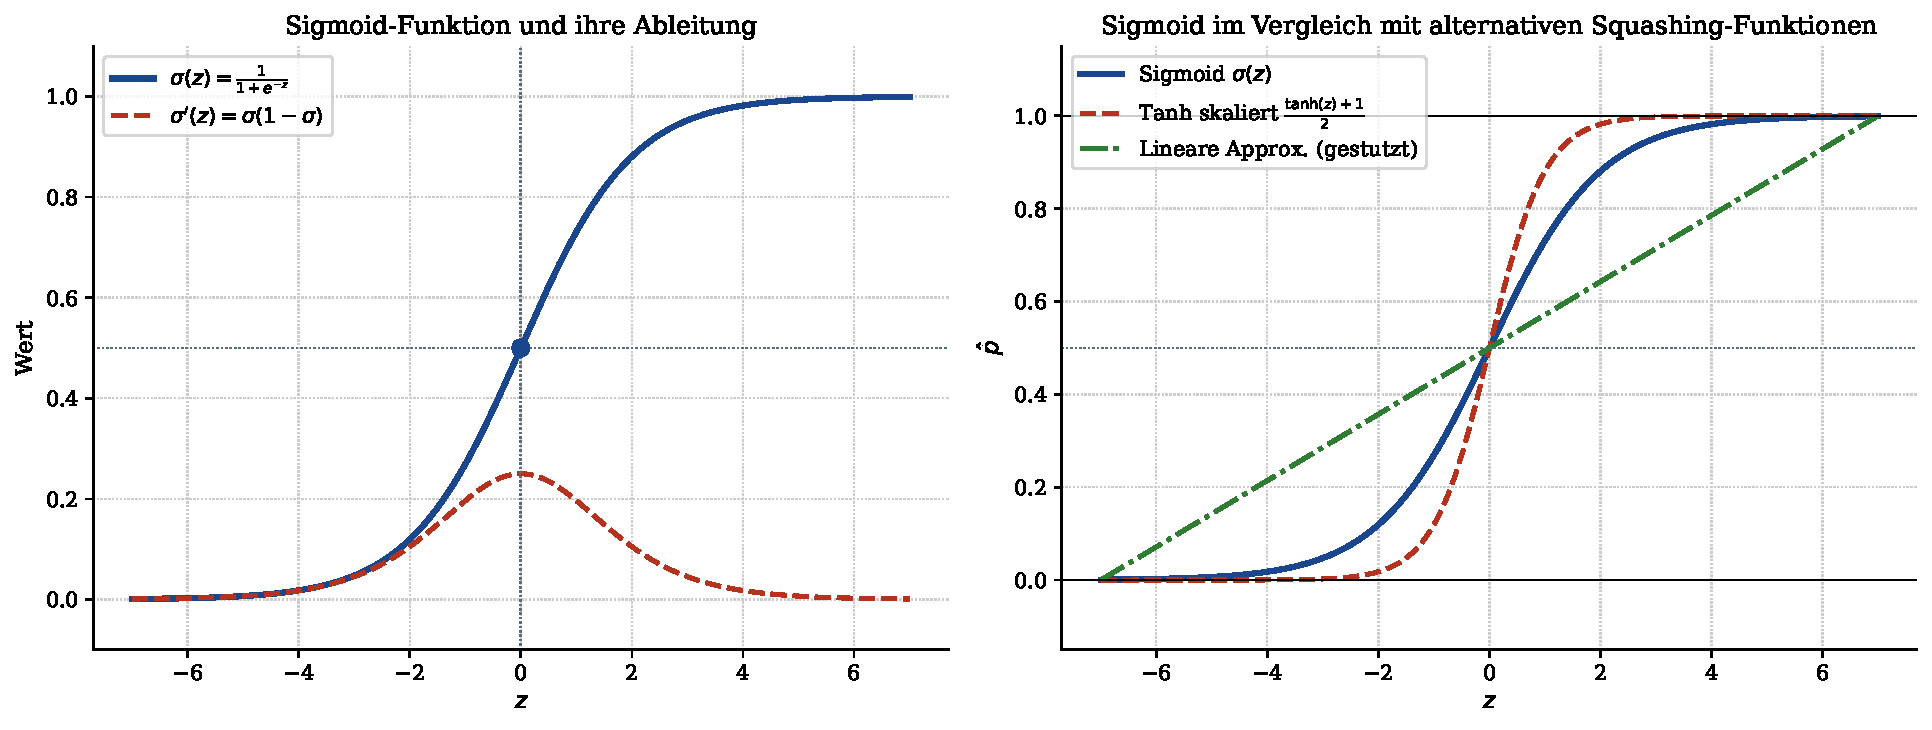
\includegraphics[width=\textwidth]{fig_sigmoid.pdf}
  \caption{Links: Sigmoid-Funktion $\sigma(z)$ und ihre Ableitung $\sigma'(z) = \sigma(z)(1-\sigma(z))$.
           Rechts: Vergleich mit alternativen Squashing-Funktionen.}
  \label{fig:sigmoid}
\end{figure}

\begin{proposition}[Eigenschaften der Sigmoid-Funktion]
  \label{prop:sigmoid_properties}
  Die Sigmoid-Funktion $\sigmoid: \R \to (0,1)$ besitzt die folgenden Eigenschaften:
  \begin{enumerate}[label=(\roman*)]
    \item \textbf{Wertebereich:} $\sigmoid : \R \to (0,1)$, streng monoton wachsend.
    \item \textbf{Symmetrie:} $\sigmoid(-z) = 1 - \sigmoid(z)$ für alle $z \in \R$.
    \item \textbf{Grenzwerte:} $\lim_{z\to+\infty}\sigmoid(z) = 1$, $\lim_{z\to-\infty}\sigmoid(z) = 0$.
    \item \textbf{Ableitung:} $\sigmoid'(z) = \sigmoid(z)\bigl(1 - \sigmoid(z)\bigr) \in (0, 1/4]$.
    \item \textbf{Inversität:} $\sigmoid^{-1}(p) = \ln\!\left(\frac{p}{1-p}\right)$ für $p \in (0,1)$ (Logit-Funktion).
    \item \textbf{Lipschitz-Stetigkeit:} $|\sigmoid(z_1) - \sigmoid(z_2)| \leq \frac{1}{4}|z_1 - z_2|$.
    \item \textbf{Zweite Ableitung:} $\sigmoid''(z) = \sigmoid(z)(1-\sigmoid(z))(1-2\sigmoid(z))$.
  \end{enumerate}
\end{proposition}

\begin{proof}
  \textbf{(iv):} Sei $f(z) = (1+e^{-z})^{-1}$. Dann:
  \[
    f'(z) = \frac{e^{-z}}{(1+e^{-z})^2}
           = \frac{1}{1+e^{-z}} \cdot \frac{e^{-z}}{1+e^{-z}}
           = \sigmoid(z) \cdot (1-\sigmoid(z)).
  \]
  Das Maximum von $\sigmoid(z)(1-\sigmoid(z))$ wird durch $\partial_z[\sigmoid(1-\sigmoid)]=0$ bestimmt:
  $\sigmoid(1-\sigmoid)(1-2\sigmoid)=0$, also bei $\sigmoid=1/2$, d.h. $z=0$, mit Wert $1/4$.

  \textbf{(vi):} Da $|\sigmoid'(z)| \leq 1/4$ für alle $z$, folgt aus dem Mittelwertsatz:
  $|\sigmoid(z_1)-\sigmoid(z_2)| \leq \sup_\xi |\sigmoid'(\xi)| \cdot |z_1-z_2| \leq \frac{1}{4}|z_1-z_2|$. 
\end{proof}

\subsection{Das Wahrscheinlichkeitsmodell}

Das logistische Regressionsmodell definiert die bedingte Wahrscheinlichkeit:

\begin{equation}
  \Prob(Y = 1 \mid \vx;\, \vw, b) = \sigmoid(\vw^\T\vx + b) =: \hat{p}(\vx),
  \label{eq:prob_model}
\end{equation}

und konseqünterweise $\Prob(Y=0 \mid \vx;\,\vw,b) = 1 - \hat{p}(\vx) = \sigmoid(-\vw^\T\vx - b)$.

\subsection{Log-Odds und Interpretierbarkeit}

\begin{proposition}[Log-Odds-Linearität]
  Unter dem logistischen Modell gilt:
  \begin{equation}
    \ln\frac{\hat{p}(\vx)}{1-\hat{p}(\vx)} = \vw^\T\vx + b.
    \label{eq:log_odds}
  \end{equation}
  Eine Erhöhung von $x_j$ um eine Einheit bei konstanten übrigen Merkmalen ergibt eine
  multiplikative Änderung der Odds um den Faktor $e^{w_j}$.
\end{proposition}

\begin{proof}
  Aus~\eqref{eq:prob_model} folgt $\hat{p} = \sigmoid(z)$ mit $z = \vw^\T\vx+b$.
  Die Logit-Transformation ergibt:
  \[
    \ln\frac{\hat{p}}{1-\hat{p}} = \ln\frac{\sigmoid(z)}{1-\sigmoid(z)}
    = \ln\frac{e^z/(1+e^z)}{1/(1+e^z)} = \ln e^z = z = \vw^\T\vx+b. \quad \square
  \]
\end{proof}

\begin{example}[Klinische Interpretation]
  In einer klinischen Studie mit $w_{\text{Alter}} = 0.05$ bedeutet dies: Pro Lebensjahr
  steigen die Odds des Erkrankungsereignisses um den Faktor $e^{0.05} \approx 1.051$, also um
  etwa $5.1\%$. Dieses Odds-Ratio ist die primäre Berichtsgrösse in epidemiologischen Studien.
\end{example}

% ============================================================
\section{Statistische Herleitung: Exponentialfamilie und GLM}
% ============================================================

\subsection{Generalisierte Lineare Modelle}

\begin{definition}[Generalisiertes Lineares Modell nach McCullagh und Nelder]
  Ein \emph{generalisiertes lineares Modell} (GLM) besteht aus drei Komponenten:
  \begin{enumerate}[label=(\roman*)]
    \item \textbf{Zufallskomponente:} $Y \mid \vx$ folgt einer Verteilung aus der Exponentialfamilie.
    \item \textbf{Systematische Komponente:} Linearer Prädiktor $z = \vw^\T\vx + b$.
    \item \textbf{Linkfunktion:} Monotone, differenzierbare Funktion $g$ mit $g(\E[Y\mid\vx]) = z$.
  \end{enumerate}
\end{definition}

Für die logistische Regression gilt: $Y\mid\vx \sim \mathrm{Bernoulli}(\hat{p})$ und die
\emph{kanonische Linkfunktion} ist der Logit $g(p) = \ln(p/(1-p))$.

\subsection{Die Bernoulli-Verteilung als Exponentialfamilie}

\begin{proposition}[Kanonische Form der Bernoulli-Verteilung]
  Die Bernoulli-Verteilung $\mathrm{Bern}(p)$ mit $p \in (0,1)$ lässt sich in der kanonischen
  Form der Exponentialfamilie schreiben:
  \begin{equation}
    f(y;\eta) = \exp\!\bigl(\eta y - A(\eta)\bigr) \cdot h(y),
    \label{eq:exp_family}
  \end{equation}
  mit kanonischem Parameter $\eta = \ln(p/(1-p)) \in \R$, Log-Partition-Funktion
  $A(\eta) = \ln(1+e^\eta)$ und Basismass $h(y) = 1$.
\end{proposition}

\begin{proof}
  Aus $f(y;p) = p^y(1-p)^{1-y}$ folgt:
  \begin{align*}
    f(y;p) &= \exp\!\bigl[y\ln p + (1-y)\ln(1-p)\bigr]
            = \exp\!\bigl[y\ln\tfrac{p}{1-p} + \ln(1-p)\bigr].
  \end{align*}
  Mit $\eta = \ln(p/(1-p))$ gilt $p = e^\eta/(1+e^\eta)$, also $1-p = 1/(1+e^\eta)$ und
  $\ln(1-p) = -\ln(1+e^\eta) = -A(\eta)$. Dies ergibt die kanonische Form~\eqref{eq:exp_family}. 
\end{proof}

\begin{proposition}[Momente aus der Log-Partition-Funktion]
  Für jede Exponentialfamilien-Verteilung gilt:
  \[
    \E[Y] = A'(\eta) = \sigmoid(\eta), \qquad \mathrm{Var}[Y] = A''(\eta) = \sigmoid(\eta)(1-\sigmoid(\eta)).
  \]
\end{proposition}

\begin{proof}
  $A'(\eta) = \frac{d}{d\eta}\ln(1+e^\eta) = \frac{e^\eta}{1+e^\eta} = \sigmoid(\eta)$.
  $A''(\eta) = \sigmoid(\eta)(1-\sigmoid(\eta))$. Die Identität $\E[T(Y)] = A'(\eta)$ gilt
  allgemein für Exponentialfamilien und folgt aus Differentiation unter dem Integral. 
\end{proof}

\subsection{Suffiziente Statistik und Informationsgeometrie}

Die Bernoulli-Verteilung gehört zur einparametrigen Exponentialfamilie mit suffizienter
Statistik $T(y) = y$. Der \emph{Fisher-Information} ist:
\begin{equation}
  \mathcal{I}(\eta) = A''(\eta) = \sigmoid(\eta)(1-\sigmoid(\eta)).
\end{equation}
Dies hat eine direkte Verbindung zur Riemannschen Metrik auf dem statistischen Mannigfaltigkeitsraum
aller Bernoulli-Verteilungen (Informationsgeometrie nach Amari~\citep{amari2016information}).

% ============================================================
\section{Verlustfunktion und Maximum-Likelihood}
% ============================================================

\subsection{Likelihood und Log-Likelihood}

Gegeben sei ein Datensatz $\mathcal{D} = \{(\vx^{(i)}, y^{(i)})\}_{i=1}^n$ mit
$y^{(i)} \in \{0,1\}$ und $\vx^{(i)} \in \R^d$. Die Likelihood-Funktion unter der
Bernoulli-Annahme mit bedingter Unabhängigkeit ist:

\begin{equation}
  L(\vw, b) = \prod_{i=1}^{n} \hat{p}_i^{\,y^{(i)}} (1-\hat{p}_i)^{1-y^{(i)}},
  \label{eq:likelihood}
\end{equation}

mit $\hat{p}_i = \sigmoid(\vw^\T\vx^{(i)}+b)$. Logarithmieren liefert die \emph{Log-Likelihood}:

\begin{equation}
  \ell(\vw, b) = \sum_{i=1}^{n}\Bigl[ y^{(i)}\ln\hat{p}_i + (1-y^{(i)})\ln(1-\hat{p}_i) \Bigr].
  \label{eq:log_likelihood}
\end{equation}

\subsection{Binäre Kreuzentropie und Informationstheorie}

\begin{definition}[Binäre Kreuzentropie-Verlustfunktion]
  \begin{equation}
    \mathcal{L}(\vw, b) = -\frac{1}{n}\sum_{i=1}^{n}\Bigl[ y^{(i)}\ln\hat{p}_i + (1-y^{(i)})\ln(1-\hat{p}_i) \Bigr].
    \label{eq:bce_loss}
  \end{equation}
\end{definition}

\begin{figure}[H]
  \centering
  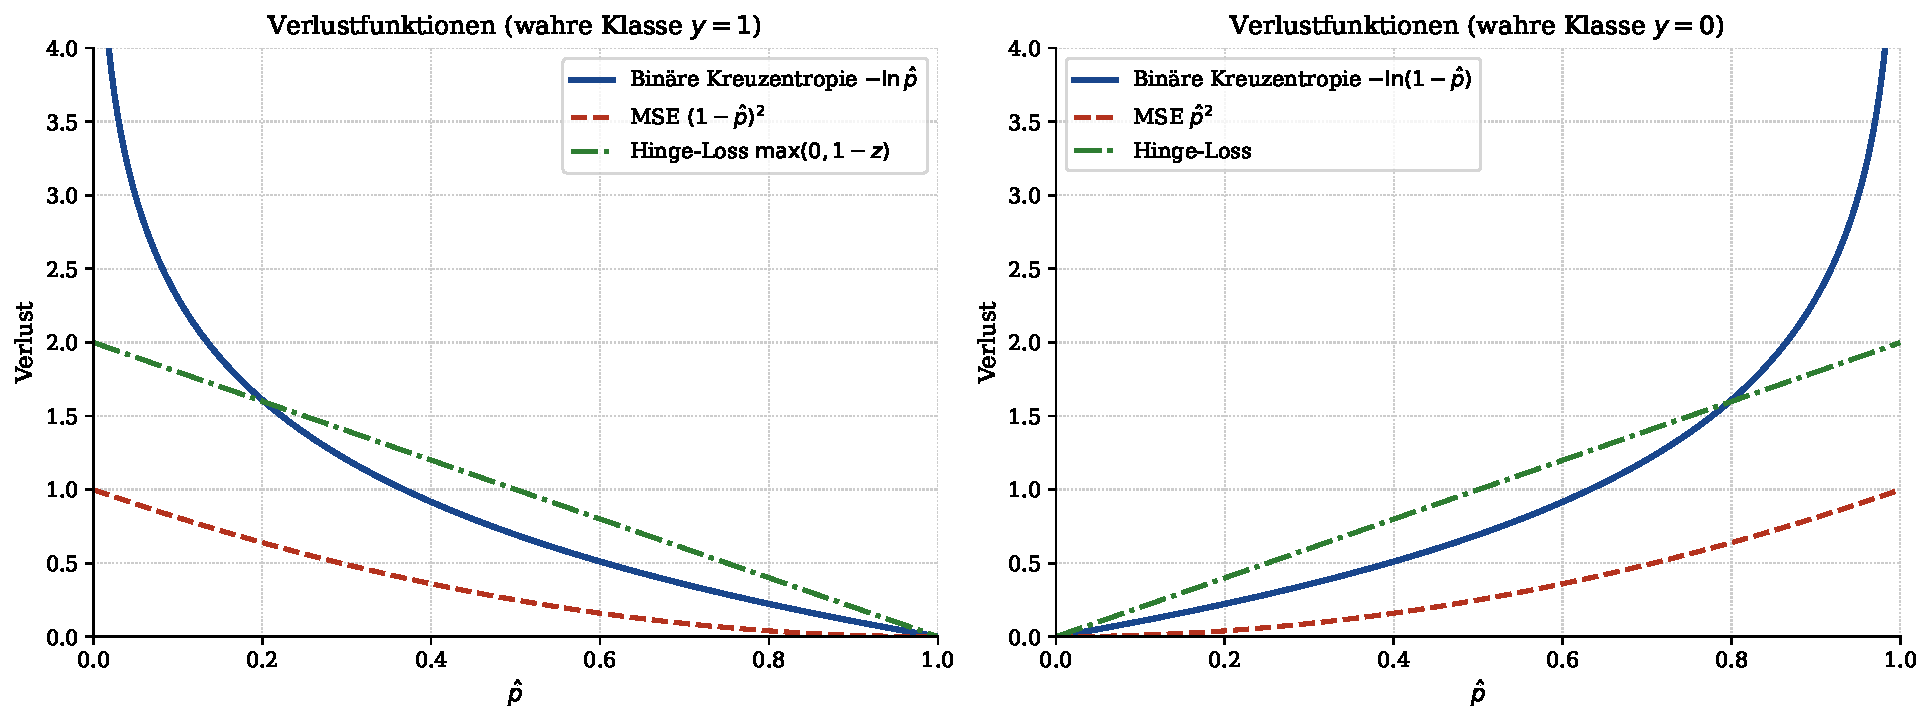
\includegraphics[width=\textwidth]{fig_loss.pdf}
  \caption{Vergleich der Verlustfunktionen (Kreuzentropie, MSE, Hinge-Loss) für beide Klassen.
           Die Kreuzentropie bestraft hochkonfidente Fehlklassifikationen am stärksten.}
  \label{fig:loss}
\end{figure}

\begin{proposition}[Informationstheoretische Interpretation]
  Die binäre Kreuzentropie ist die \emph{Kreuzentropie} zwischen der empirischen Verteilung
  $q_i = y^{(i)}$ und der Modellverteilung $\hat{p}_i$:
  \[
    \mathcal{L} = \frac{1}{n}\sum_{i=1}^n H(q_i, \hat{p}_i)
    = \frac{1}{n}\sum_{i=1}^n \bigl[H(q_i) + \KL(q_i \| \hat{p}_i)\bigr],
  \]
  wobei $H(q_i)$ die binäre Entropie der wahren Verteilung und $\KL(q_i\|\hat{p}_i)$ die
  Kullback-Leibler-Divergenz bezeichnen. Da $H(q_i)$ nicht von den Parametern abhängt, ist
  die Minimierung der Kreuzentropie äquivalent zur Minimierung der KL-Divergenz.
\end{proposition}

\subsection{Konvexität der Verlustfunktion}

\begin{theorem}[Konvexität der binären Kreuzentropie]
  \label{thm:convexity}
  Die Verlustfunktion $\mathcal{L}(\vw, b): \R^{d+1} \to \R$ aus~\eqref{eq:bce_loss} ist
  konvex in $(\vw, b)$.
\end{theorem}

\begin{proof}
  Wir zeigen positive Semidefinitheit der Hesse-Matrix. Sei $\tilde{\vw} = (b, \vw)^\T \in \R^{d+1}$
  und $\tilde{\vx}^{(i)} = (1, {\vx^{(i)}}^\T)^\T$. Für den $i$-ten Term der Verlustfunktion gilt:
  \[
    \ell_i(\tilde{\vw}) = -y^{(i)}\ln\sigmoid(z_i) - (1-y^{(i)})\ln(1-\sigmoid(z_i)), \quad z_i = \tilde{\vw}^\T\tilde{\vx}^{(i)}.
  \]
  Erste Ableitung nach $z_i$:
  \[
    \frac{\partial \ell_i}{\partial z_i} = \sigmoid(z_i) - y^{(i)}.
  \]
  Zweite Ableitung:
  \[
    \frac{\partial^2 \ell_i}{\partial z_i^2} = \sigmoid(z_i)(1-\sigmoid(z_i)) =: s_i \geq 0.
  \]
  Die Hesse-Matrix von $\mathcal{L}$ bzgl. $\tilde{\vw}$ ist:
  \begin{equation}
    \nabla^2 \mathcal{L} = \frac{1}{n}\sum_{i=1}^n s_i \tilde{\vx}^{(i)}\bigl(\tilde{\vx}^{(i)}\bigr)^{\top}
    = \frac{1}{n} \tilde{\vX}^\T \vS \tilde{\vX},
    \label{eq:hessian}
  \end{equation}
  wobei $\tilde{\vX} \in \R^{n \times (d+1)}$ die augmentierte Designmatrix und
  $\vS = \diag(s_1, \ldots, s_n) \succeq 0$ ist. Für jeden Vektor $\bm{v} \in \R^{d+1}$ gilt:
  \[
    \bm{v}^\T \nabla^2 \mathcal{L}\, \bm{v}
    = \frac{1}{n}\sum_{i=1}^n s_i (\tilde{\vx}^{(i)\T}\bm{v})^2 \geq 0,
  \]
  da $s_i \geq 0$. Also ist $\nabla^2\mathcal{L} \succeq 0$, was die Konvexität beweist.
  Strikte Konvexität gilt genau dann, wenn $\tilde{\vX}$ vollen Spaltenrang hat und
  mindestens ein $s_i > 0$ ist. 
\end{proof}

\begin{corollary}
  Jedes lokale Minimum von $\mathcal{L}$ ist ein globales Minimum. Wenn $\tilde{\vX}$ vollen
  Spaltenrang hat, ist das Minimum eindeutig (sofern es endlich ist; bei linear separierbaren
  Daten existiert kein endliches Minimum).
\end{corollary}

\subsection{Gradientenberechnung}

\begin{proposition}[Gradient der binären Kreuzentropie]
  \begin{align}
    \nabla_{\vw} \mathcal{L} &= \frac{1}{n}\sum_{i=1}^n (\hat{p}_i - y^{(i)})\vx^{(i)}
    = \frac{1}{n}\vX^\T(\vp - \vy),
    \label{eq:gradient_w} \\
    \frac{\partial \mathcal{L}}{\partial b} &= \frac{1}{n}\sum_{i=1}^n (\hat{p}_i - y^{(i)}).
    \label{eq:gradient_b}
  \end{align}
\end{proposition}

\begin{proof}
  Wir leiten den $i$-ten Beitrag nach $w_k$ ab:
  \begin{align*}
    \frac{\partial \ell_i}{\partial w_k}
    &= \frac{\partial}{\partial w_k}\bigl[-y^{(i)}\ln\sigmoid(z_i) - (1-y^{(i)})\ln(1-\sigmoid(z_i))\bigr] \\
    &= \bigl(\sigmoid(z_i) - y^{(i)}\bigr)\frac{\partial z_i}{\partial w_k}
     = (\hat{p}_i - y^{(i)}) x_k^{(i)}.
  \end{align*}
  Summation und Division durch $n$ ergibt~\eqref{eq:gradient_w}. 
\end{proof}

\begin{remark}[Elegante Gradientenstruktur]
  Der Gradient hat die Form $\frac{1}{n}\vX^\T(\vp - \vy)$: Er ist die mittlere Differenz
  zwischen Vorhersage und Wahrheit, gewichtet mit den Merkmalen. Diese Struktur ist identisch
  mit dem Gradienten der linearen Regression (dort: $\frac{1}{n}\vX^\T(\hat{\vy}-\vy)$) --
  mit dem einzigen Unterschied, dass $\hat{\vy}$ durch die Sigmoid-Transformation ersetzt wird.
\end{remark}

% ============================================================
\section{Optimierungsverfahren}
% ============================================================

\subsection{Gradientenabstieg}

\begin{algorithm}[H]
  \caption{Batch-Gradientenabstieg für logistische Regression}
  \label{alg:gd}
  \begin{algorithmic}[1]
    \Require Datensatz $\mathcal{D}$, Lernrate $\eta > 0$, Toleranz $\epsilon > 0$, Max. Iterationen $T$
    \Ensure Parameterschätzer $\hat{\vw}$, $\hat{b}$
    \State Initialisiere $\vw \leftarrow \mathbf{0} \in \R^d$, $b \leftarrow 0$
    \For{$t = 1, 2, \ldots, T$}
      \State $z_i \leftarrow \vw^\T\vx^{(i)}+b$ für alle $i = 1,\ldots,n$
      \State $\hat{p}_i \leftarrow \sigmoid(z_i)$ für alle $i$
      \State $\mathbf{g}_{\vw} \leftarrow \frac{1}{n}\vX^\T(\vp-\vy)$; \quad $g_b \leftarrow \frac{1}{n}\mathbf{1}^\T(\vp-\vy)$
      \State $\vw \leftarrow \vw - \eta \mathbf{g}_{\vw}$; \quad $b \leftarrow b - \eta g_b$
      \If{$\|\mathbf{g}_{\vw}\|_2 < \epsilon$} \textbf{break} \EndIf
    \EndFor
  \end{algorithmic}
\end{algorithm}

\begin{theorem}[Konvergenz des Gradientenabstiegs]
  \label{thm:gd_convergence}
  Sei $\mathcal{L}$ strikt konvex mit $L$-Lipschitz-stetigem Gradienten
  ($\|\nabla\mathcal{L}(\vw_1)-\nabla\mathcal{L}(\vw_2)\|\leq L\|\vw_1-\vw_2\|$).
  Dann konvergiert der Gradientenabstieg mit konstanter Lernrate $\eta \leq 1/L$ linear:
  \begin{equation}
    \mathcal{L}(\vw^{(t)}) - \mathcal{L}(\vw^*) \leq (1-\mu\eta)^t \bigl[\mathcal{L}(\vw^{(0)}) - \mathcal{L}(\vw^*)\bigr],
    \label{eq:gd_convergence}
  \end{equation}
  wobei $\mu > 0$ der kleinste Eigenwert der Hesse-Matrix (Starke-Konvexitäts-Parameter) ist.
\end{theorem}

\begin{proof}
  Da $\mathcal{L}$ $L$-glatt ist, gilt für alle $\vw, \tilde{\vw}$:
  \[
    \mathcal{L}(\tilde{\vw}) \leq \mathcal{L}(\vw) + \nabla\mathcal{L}(\vw)^\T(\tilde{\vw}-\vw)
    + \frac{L}{2}\|\tilde{\vw}-\vw\|^2.
  \]
  Setze $\tilde{\vw} = \vw - \eta\nabla\mathcal{L}(\vw)$:
  \[
    \mathcal{L}(\vw^{(t+1)}) \leq \mathcal{L}(\vw^{(t)}) - \eta\bigl(1-\tfrac{\eta L}{2}\bigr)
    \|\nabla\mathcal{L}(\vw^{(t)})\|^2.
  \]
  Aus starker Konvexität folgt $\|\nabla\mathcal{L}(\vw)\|^2 \geq 2\mu[\mathcal{L}(\vw)-\mathcal{L}(\vw^*)]$.
  Rekursive Anwendung ergibt~\eqref{eq:gd_convergence}. 
\end{proof}

\begin{figure}[H]
  \centering
  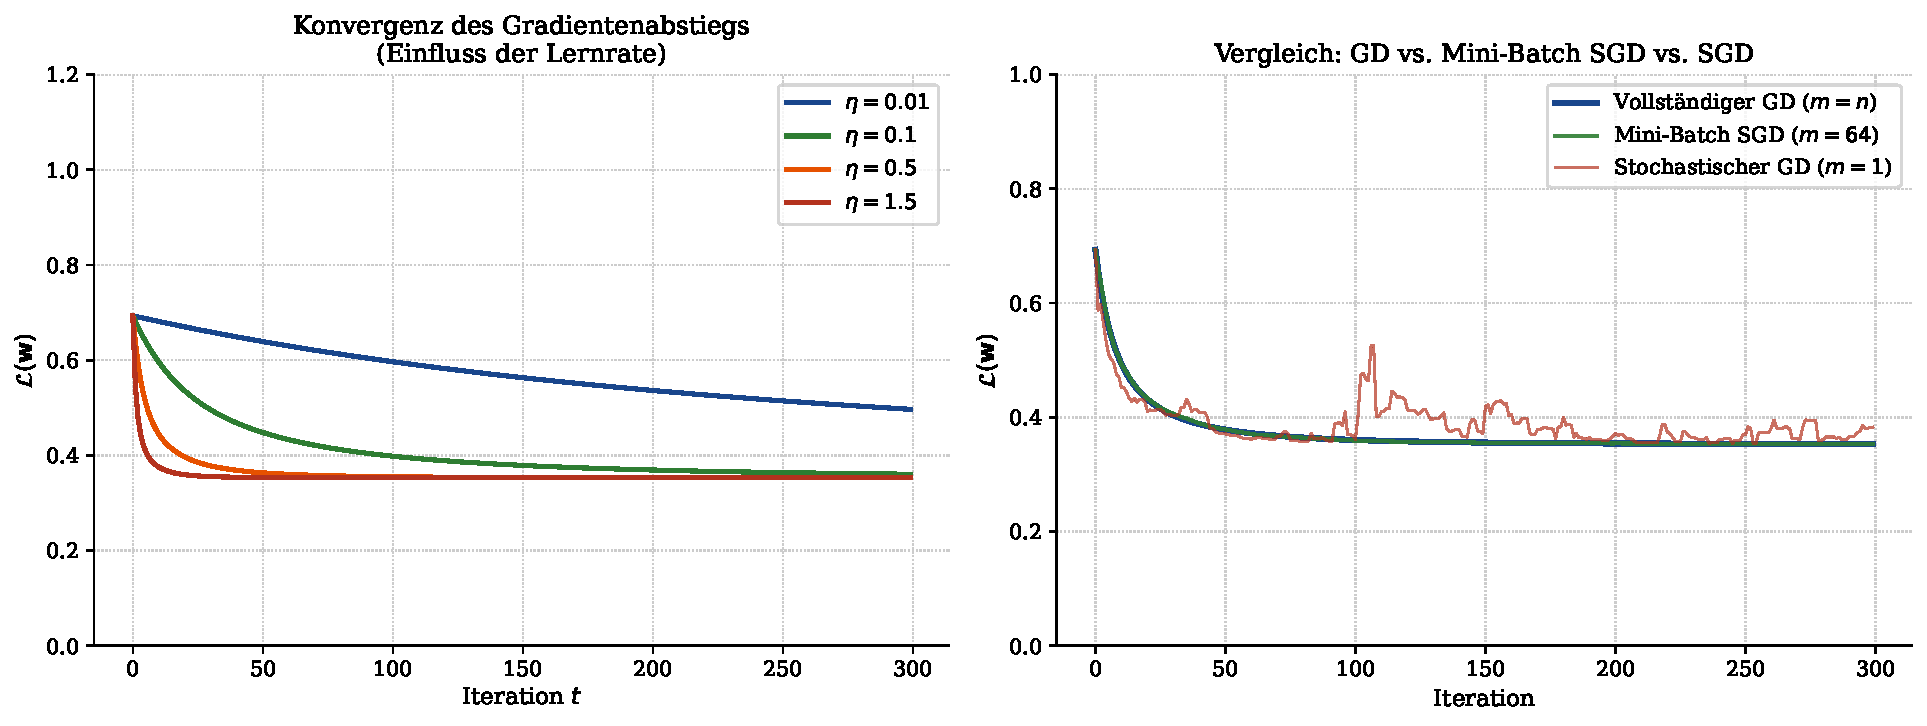
\includegraphics[width=\textwidth]{fig_optimization.pdf}
  \caption{Links: Einfluss der Lernrate auf die Konvergenzgeschwindigkeit. Zu grosse Lernraten
           führen zur Divergenz. Rechts: Vergleich zwischen vollständigem GD, Mini-Batch SGD
           und stochastischem GD.}
  \label{fig:optimization}
\end{figure}

\subsection{Newton-Raphson-Verfahren (IRLS)}

Das Newton-Verfahren nutzt die Hesse-Matrix für quadratisch konvergente Updates:

\begin{equation}
  \tilde{\vw}^{(t+1)} \leftarrow \tilde{\vw}^{(t)} - \bigl(\nabla^2\mathcal{L}\bigr)^{-1}\nabla\mathcal{L}.
  \label{eq:newton}
\end{equation}

\begin{theorem}[Newton-Raphson als IRLS]
  Das Newton-Raphson-Verfahren für die logistische Regression ist äquivalent zum
  \emph{Iteratively Reweighted Least Squares} (IRLS): In jeder Iteration wird ein gewichtetes
  lineares Kleinste-Quadrate-Problem der Form
  \begin{equation}
    \tilde{\vw}^{(t+1)} = (\tilde{\vX}^\T \vS^{(t)} \tilde{\vX})^{-1} \tilde{\vX}^\T \vS^{(t)} \bm{\zeta}^{(t)}
    \label{eq:irls}
  \end{equation}
  gelöst, mit Gewichtsmatrix $\vS^{(t)} = \diag(s_i^{(t)})$, $s_i^{(t)} = \hat{p}_i^{(t)}(1-\hat{p}_i^{(t)})$,
  und angepasster Antwortvariable $\zeta_i^{(t)} = z_i^{(t)} + (y^{(i)} - \hat{p}_i^{(t)})/s_i^{(t)}$.
\end{theorem}

\begin{proof}
  Aus der Newton-Update-Regel folgt mit der Hesse-Matrix~\eqref{eq:hessian} und dem Gradienten:
  \begin{align*}
    \tilde{\vw}^{(t+1)}
    &= \tilde{\vw}^{(t)} - \frac{1}{n}(\tilde{\vX}^\T\vS\tilde{\vX})^{-1} \cdot \frac{1}{n}\tilde{\vX}^\T(\vp-\vy) \cdot n \\
    &= (\tilde{\vX}^\T\vS\tilde{\vX})^{-1}\tilde{\vX}^\T\vS \bigl[\tilde{\vX}\tilde{\vw}^{(t)} + \vS^{-1}(\vy-\vp)\bigr]
    = (\tilde{\vX}^\T\vS\tilde{\vX})^{-1}\tilde{\vX}^\T\vS\bm{\zeta},
  \end{align*}
  was~\eqref{eq:irls} ergibt. 
\end{proof}

\begin{theorem}[Quadratische Konvergenz von Newton-Raphson]
  Sei $\vw^*$ das einzige Minimum von $\mathcal{L}$ und $\nabla^2\mathcal{L}(\vw^*)$ positiv definit
  mit kleinstem Eigenwert $\mu > 0$. Dann gilt lokal:
  \begin{equation}
    \|\vw^{(t+1)} - \vw^*\| \leq \frac{M}{2\mu} \|\vw^{(t)} - \vw^*\|^2,
    \label{eq:newton_convergence}
  \end{equation}
  wobei $M = \sup_{\vw} \|\nabla^3\mathcal{L}(\vw)\|$ die Lipschitz-Konstante der Hesse-Matrix bezeichnet.
\end{theorem}

\subsection{L-BFGS: Quasi-Newton-Methode für grosse Dimensionen}

Für hochdimensionale Probleme ($d \gg 1$) ist die explizite Berechnung und Invertierung der
$(d+1)\times(d+1)$-Hesse-Matrix unpraktikabel. Das \emph{Limited-memory Broyden-Fletcher-Goldfarb-Shanno}
(L-BFGS) Verfahren approximiert die inverse Hesse-Matrix durch die letzten $m$ (typisch $m=5-20$)
Gradientendifferenzen:
\begin{equation}
  H_k^{-1} \approx V_k^\T \cdots V_{k-m}^\T H_0^{-1} V_{k-m} \cdots V_k + \text{Rang-}2m\text{-Korrekturen},
\end{equation}
mit $V_k = I - \rho_k \bm{s}_k\bm{y}_k^\T$, $\rho_k = 1/(\bm{y}_k^\T\bm{s}_k)$,
$\bm{s}_k = \vw^{(k)}-\vw^{(k-1)}$, $\bm{y}_k = \nabla\mathcal{L}(\vw^{(k)})-\nabla\mathcal{L}(\vw^{(k-1)})$.

\subsection{Stochastischer Gradientenabstieg und Varianten}

\begin{algorithm}[H]
  \caption{Adam-Optimizer für logistische Regression}
  \label{alg:adam}
  \begin{algorithmic}[1]
    \Require Lernrate $\alpha$, $\beta_1, \beta_2 \in [0,1)$, $\epsilon > 0$, Datensatz $\mathcal{D}$
    \State $\bm{m}_0 \leftarrow 0$, $\bm{v}_0 \leftarrow 0$, $t \leftarrow 0$
    \While{nicht konvergiert}
      \State $t \leftarrow t+1$
      \State Berechne Gradient $\bm{g}_t = \nabla_{\vw}\mathcal{L}$ auf Mini-Batch
      \State $\bm{m}_t \leftarrow \beta_1 \bm{m}_{t-1} + (1-\beta_1)\bm{g}_t$ \hfill (1. Moment)
      \State $\bm{v}_t \leftarrow \beta_2 \bm{v}_{t-1} + (1-\beta_2)\bm{g}_t^2$ \hfill (2. Moment)
      \State $\hat{\bm{m}}_t \leftarrow \bm{m}_t/(1-\beta_1^t)$; $\hat{\bm{v}}_t \leftarrow \bm{v}_t/(1-\beta_2^t)$
      \State $\vw \leftarrow \vw - \alpha \hat{\bm{m}}_t/(\sqrt{\hat{\bm{v}}_t}+\epsilon)$
    \EndWhile
  \end{algorithmic}
\end{algorithm}

% ============================================================
\section{Entscheidungsgrenze und geometrische Interpretation}
% ============================================================

\subsection{Lineare Entscheidungsgrenze}

\begin{definition}[Entscheidungsgrenze]
  Die \emph{Entscheidungsgrenze} mit Schwellwert $\tau \in (0,1)$ ist die Hyperebene:
  \[
    \mathcal{H}_\tau = \bigl\{\vx \in \R^d : \vw^\T\vx + b = \ln\tfrac{\tau}{1-\tau} \bigr\}.
  \]
  Für $\tau=0.5$: $\mathcal{H}_{0.5} = \{\vx : \vw^\T\vx + b = 0\}$.
\end{definition}

\begin{figure}[H]
  \centering
  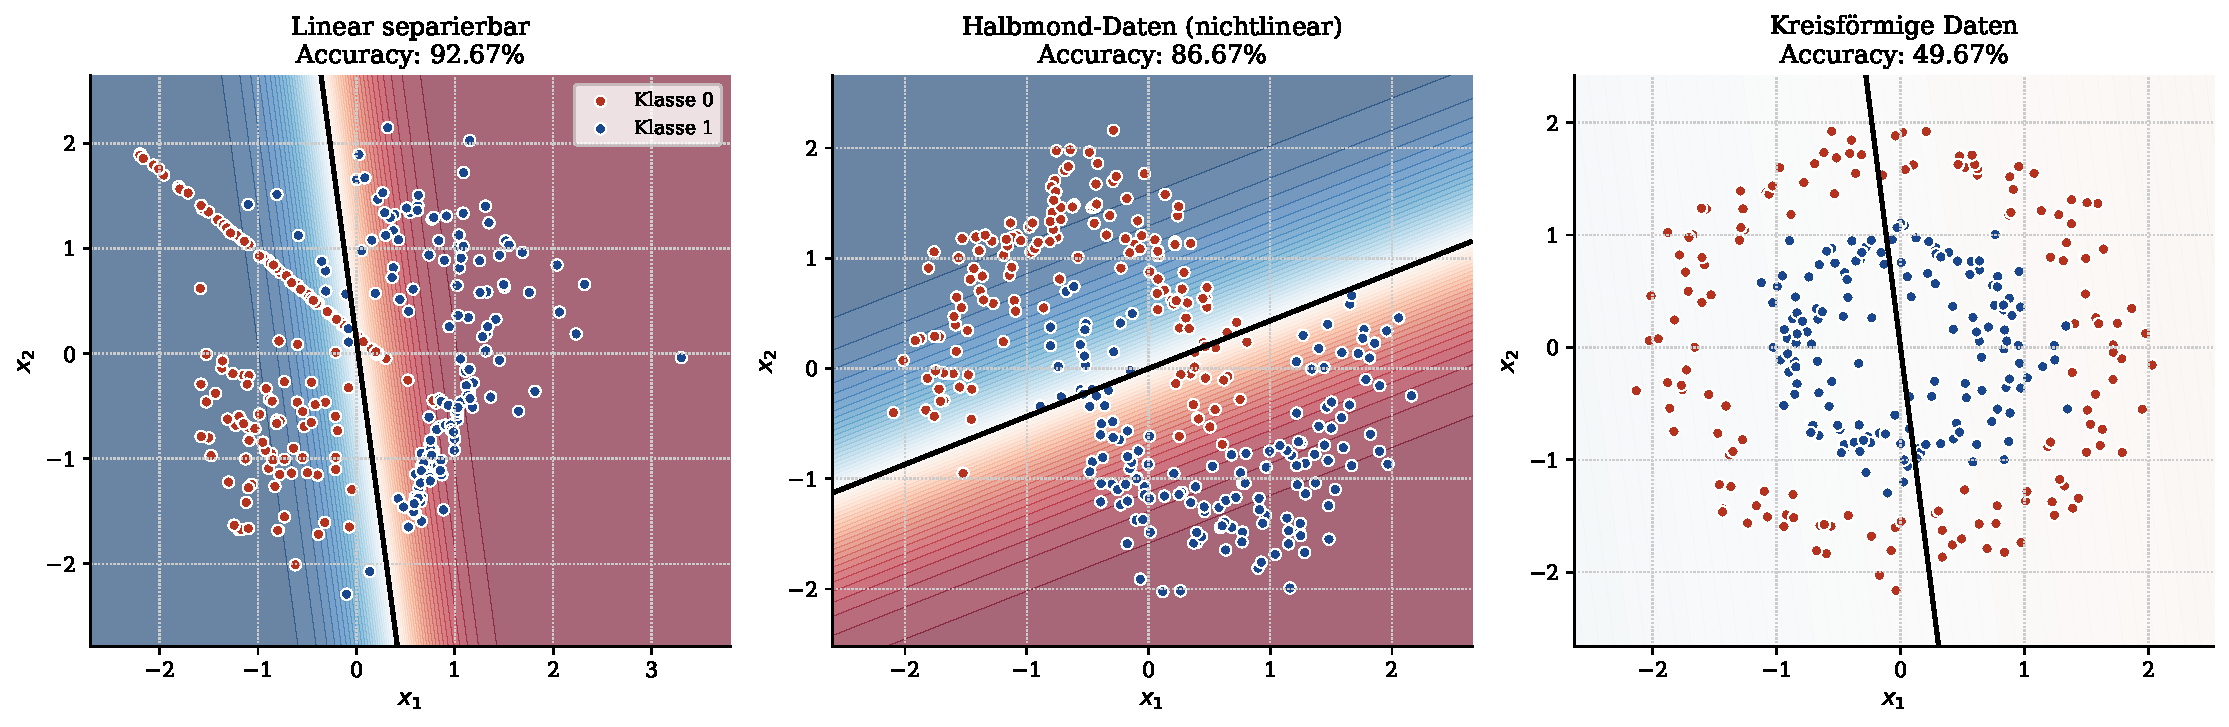
\includegraphics[width=\textwidth]{fig_decision.pdf}
  \caption{Entscheidungsgrenzen der logistischen Regression. Links: linear separierbare Daten
           mit gerader Trennlinie. Mitte und rechts: nichtlinear verteilte Daten, bei denen
           die lineare Entscheidungsgrenze versagt.}
  \label{fig:decision}
\end{figure}

\begin{proposition}[Geometrie der Entscheidungsgrenze]
  Die Entscheidungsgrenze $\mathcal{H}_{0.5}$ ist eine $(d-1)$-dimensionale Hyperebene mit
  Normalenvektor $\vw$ und vorzeichenbehaftetem Abstand des Punktes $\vx_0$ von der Grenze:
  \begin{equation}
    d(\vx_0, \mathcal{H}) = \frac{\vw^\T\vx_0 + b}{\|\vw\|_2}.
    \label{eq:margin}
  \end{equation}
\end{proposition}

\subsection{Margin und Konfidenz}

Der vorzeichenbehaftete Abstand~\eqref{eq:margin} misst die Klassifikationskonfidenz:
Je grösser $|d(\vx_0,\mathcal{H})|$, desto weiter ist der Punkt von der Entscheidungsgrenze
entfernt und desto sicherer ist die Vorhersage. Bei $|d| \to \infty$ nähert sich $\hat{p}$
asymptotisch 1 (oder 0) an.

\subsection{Nicht-lineare Erweiterung durch Feature-Maps}

\begin{definition}[Kernel-Logistische Regression]
  Sei $\phi: \R^d \to \mathcal{H}$ eine Feature-Map in einen (möglicherweise unendlichdimensionalen)
  Hilbert-Raum $\mathcal{H}$. Die Kernel-Logistische Regression modelliert:
  \[
    \hat{p}(\vx) = \sigmoid(\langle\vw, \phi(\vx)\rangle_{\mathcal{H}} + b).
  \]
  Der \emph{Representer-Satz} garantiert, dass die Lösung die Form
  $\vw = \sum_{i=1}^n \alpha_i \phi(\vx^{(i)})$ hat, was die Auswertung via Kernel
  $k(\vx, \vx') = \langle\phi(\vx),\phi(\vx')\rangle$ ermöglicht.
\end{definition}

% ============================================================
\section{Regularisierung}
% ============================================================

\subsection{Ridge-Regularisierung (L2)}

\begin{equation}
  \mathcal{L}_{\lambda_2}(\vw, b) = \mathcal{L}(\vw,b) + \frac{\lambda_2}{2}\|\vw\|_2^2.
  \label{eq:l2_loss}
\end{equation}

\begin{proposition}[Bayesianische Interpretation der L2-Regularisierung]
  L2-Regularisierung entspricht einer \emph{Maximum a Posteriori} (MAP)-Schätzung mit
  Gauss'schem Prior $p(\vw) = \mathcal{N}(\mathbf{0}, \lambda_2^{-1}\mathbf{I})$:
  \[
    \hat{\vw}_{\mathrm{MAP}} = \arg\max_{\vw} \bigl[\ln L(\vw) + \ln p(\vw)\bigr]
    = \arg\min_{\vw} \Bigl[\mathcal{L}(\vw) + \tfrac{\lambda_2}{2}\|\vw\|_2^2\Bigr].
  \]
\end{proposition}

\begin{proof}
  Mit $\ln p(\vw) = -\frac{\lambda_2}{2}\|\vw\|_2^2 + \mathrm{const}$ gilt:
  $\arg\max\bigl[\ell(\vw) - \frac{\lambda_2}{2}\|\vw\|_2^2\bigr] = \arg\min\mathcal{L}_{\lambda_2}(\vw)$. 
\end{proof}

\subsection{Lasso-Regularisierung (L1)}

\begin{equation}
  \mathcal{L}_{\lambda_1}(\vw, b) = \mathcal{L}(\vw,b) + \lambda_1\|\vw\|_1,
  \quad \|\vw\|_1 = \sum_{j=1}^d |w_j|.
  \label{eq:l1_loss}
\end{equation}

\begin{proposition}[Sparsitätsinduktion durch L1]
  Die L1-regularisierte Verlustfunktion hat die Eigenschaft, dass für genügend grosse $\lambda_1$
  bestimmte Köffizienzen exakt zu Null gesetzt werden (Sparsität). Die Karush-Kuhn-Tucker-
  Bedingungen für ein Minimum $\hat{\vw}$ lauten:
  \[
    \frac{\partial \mathcal{L}}{\partial w_j} + \lambda_1 \sign(w_j) = 0 \quad (w_j \neq 0),
    \qquad \left|\frac{\partial \mathcal{L}}{\partial w_j}\right| \leq \lambda_1 \quad (w_j = 0).
  \]
\end{proposition}

\begin{figure}[H]
  \centering
  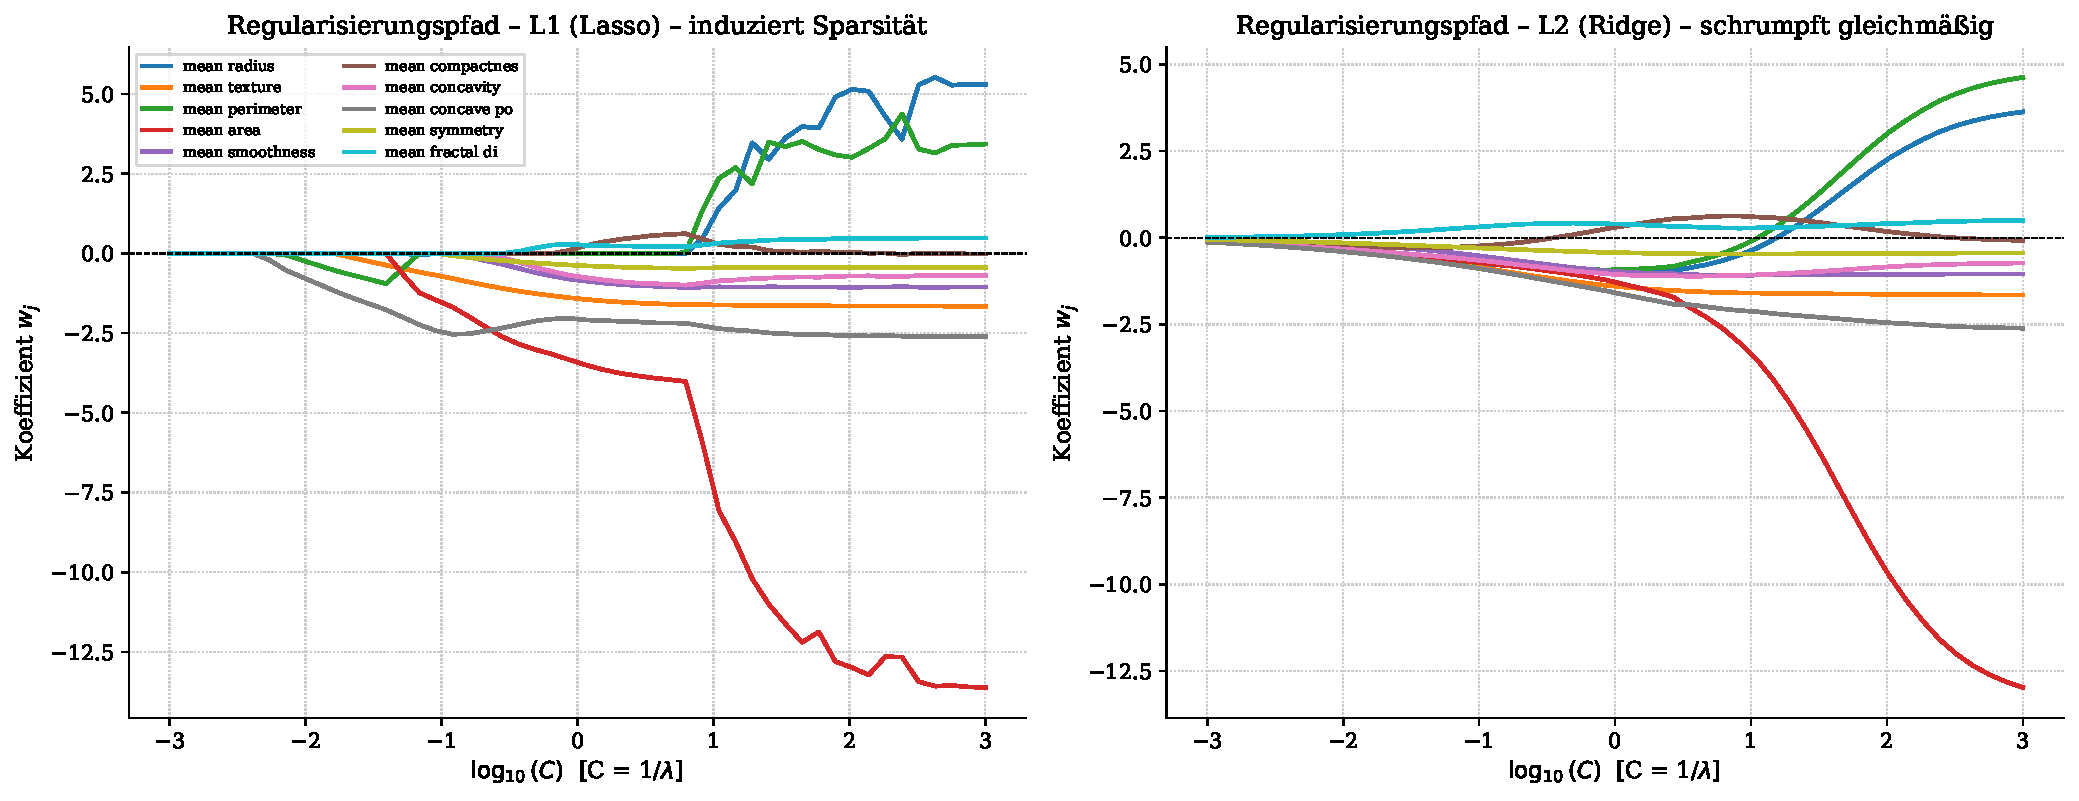
\includegraphics[width=\textwidth]{fig_regularization.pdf}
  \caption{Regularisierungspfade. Links: L1-Regularisierung setzt Köffizienzen exakt auf Null
           (Sparsität). Rechts: L2-Regularisierung schrumpft alle Köffizienzen gleichmässig
           ohne vollständige Elimination.}
  \label{fig:regularization}
\end{figure}

\subsection{Elastic Net}

\begin{equation}
  \mathcal{L}_{\mathrm{EN}}(\vw) = \mathcal{L}(\vw) + \lambda_1\|\vw\|_1 + \frac{\lambda_2}{2}\|\vw\|_2^2.
\end{equation}

\begin{table}[H]
  \centering
  \caption{Vergleich der Regularisierungsverfahren für logistische Regression.}
  \begin{tabular}{lccccl}
    \toprule
    Methode & Strafterm & Sparsit. & Diff'bar & Prior & Typ. Anwendungsfall \\
    \midrule
    Keine    & --                                     & Nein & Ja  & Uniform           & Kleine $n$, linear separ. \\
    L2 Ridge & $\lambda\|\vw\|_2^2$                   & Nein & Ja  & Gaussisch         & Korrelierte Merkmale \\
    L1 Lasso & $\lambda\|\vw\|_1$                     & Ja   & Nein & Laplace          & Hochdimens. Daten \\
    Elastic  & $\lambda_1\|\vw\|_1+\lambda_2\|\vw\|_2^2$ & Ja & Nein & Gemischt       & Gruppen korr. Merkm. \\
    \bottomrule
  \end{tabular}
  \label{tab:regularization}
\end{table}

\begin{figure}[H]
  \centering
  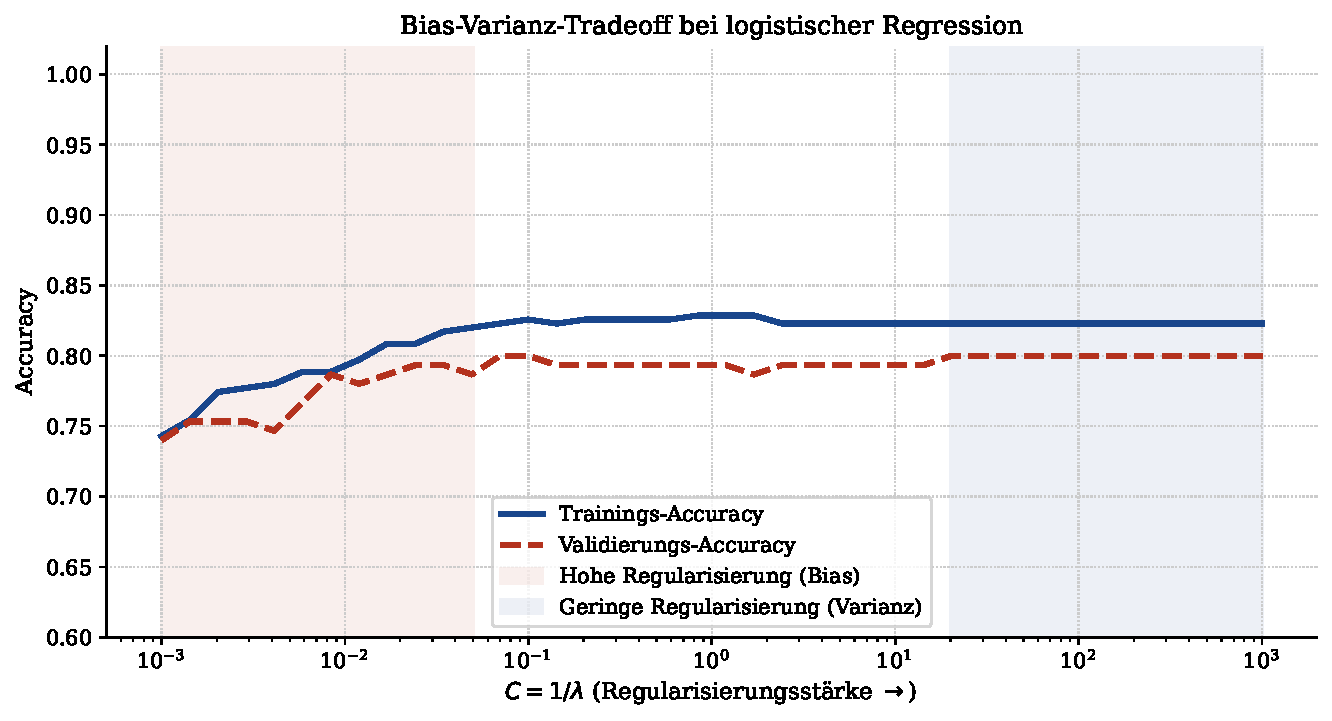
\includegraphics[width=0.7\textwidth]{fig_biasvariance.pdf}
  \caption{Bias-Varianz-Tradeoff: Starke Regularisierung ($C$ klein) führt zu hohem Bias
           (Underfitting), schwache Regularisierung ($C$ gross) zu hoher Varianz (Overfitting).}
  \label{fig:biasvariance}
\end{figure}


% ============================================================
\section{Varianzinflationsfaktor (VIF) und Multikollinearität}
\label{sec:vif}
% ============================================================

Eines der zentralen Qualitätsprobleme in der logistischen Regression -- wie auch in der 
linearen Regression -- ist die \emph{Multikollinearität} zwischen Prädiktorvariablen. 
Wenn Eingabemerkmale stark miteinander korrelieren, werden die geschätzten Regressionsköffizienten 
instabil, ihre Varianzen aufgeblasen und ihre Interpretierbarkeit fundamental beeinträchtigt. 
Der \emph{Varianzinflationsfaktor} (VIF, engl.\@ \textit{Variance Inflation Factor}) ist das 
meistverwendete diagnostische Instrument zur Quantifizierung dieses Problems. Dieses Kapitel 
entwickelt die mathematischen Grundlagen des VIF, seine Berechnung, Interpretation und 
praktische Bedeutung für die logistische Regression in vollständiger Tiefe.

% ------------------------------------------------------------
\subsection{Motivation: Das Problem der Multikollinearität}
% ------------------------------------------------------------

\begin{definition}[Multikollinearität]
	Seien $\vx_1, \vx_2, \ldots, \vx_d \in \R^n$ die Spalten der Designmatrix $\vX \in \R^{n \times d}$.
	\emph{Exakte Multikollinearität} liegt vor, wenn es einen Vektor $\bm{c} = (c_1, \ldots, c_d)^\T \neq \bm{0}$
	gibt mit
	\[
	\sum_{j=1}^{d} c_j \vx_j = \bm{0},
	\]
	d.\,h.\ wenn $\vX$ nicht vollen Spaltenrang hat. \emph{Approximative Multikollinearität} liegt vor,
	wenn diese Beziehung näherungsweise gilt, also $\|\sum_j c_j \vx_j\|_2 \approx 0$ für ein
	nichttriviales $\bm{c}$.
\end{definition}

\begin{remark}[Konseqünzen exakter Multikollinearität]
	Bei exakter Multikollinearität ist die Designmatrix $\vX^\T\vX$ singulär. Die 
	Normalengleichungen der linearen Regression besitzen dann unendlich viele Lösungen, 
	und der Maximum-Likelihood-Schätzer der logistischen Regression existiert nicht eindeutig. 
	In der Praxis ist approximative Multikollinearität das weitaus häufigere und 
	gleichzeitig schwerer zu diagnostizierende Problem.
\end{remark}

Um das Problem zu verstehen, betrachten wir den Standardfehler eines Regressionsköffizienten.
Im linearen Regressionsmodell $\vy = \vX\vw + \bm{\varepsilon}$ mit $\bm{\varepsilon} \sim \mathcal{N}(\bm{0}, \sigma^2\mathbf{I})$
ist die Kovarianzmatrix des OLS-Schätzers $\hat{\vw} = (\vX^\T\vX)^{-1}\vX^\T\vy$:
\begin{equation}
	\mathrm{Cov}(\hat{\vw}) = \sigma^2 (\vX^\T\vX)^{-1}.
	\label{eq:cov_ols}
\end{equation}
Insbesondere ist die Varianz des $j$-ten Köffizienten:
\begin{equation}
	\mathrm{Var}(\hat{w}_j) = \sigma^2 \bigl[(\vX^\T\vX)^{-1}\bigr]_{jj}.
	\label{eq:var_cöff}
\end{equation}
Wenn Spalten von $\vX$ stark korreliert sind, werden die Diagonalelemente von $(\vX^\T\vX)^{-1}$
sehr groß, was zu großen Standardfehlern, breiten Konfidenzintervallen und damit zur
Unzuverlässigkeit der Köffizienten führt -- selbst wenn das Modell als Ganzes eine gute
Vorhersagequalität besitzt.

\begin{figure}[H]
	\centering
	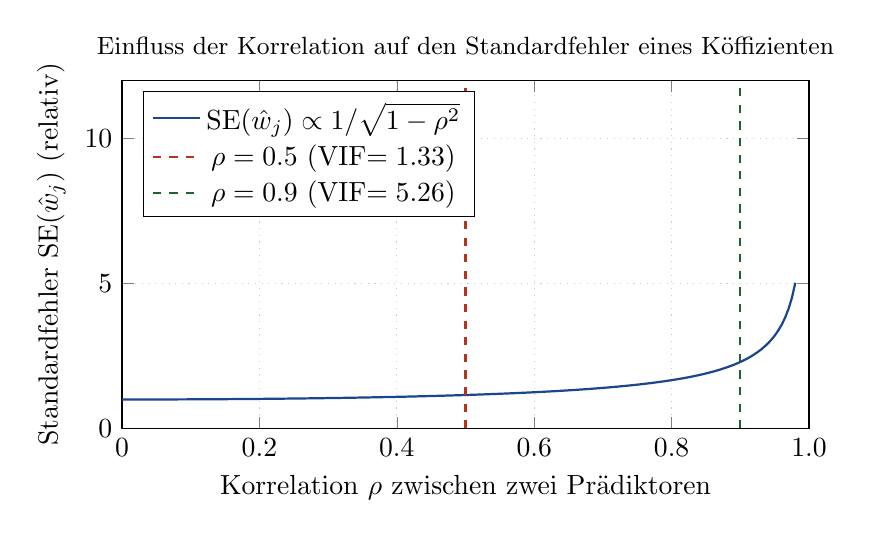
\begin{tikzpicture}
		\begin{axis}[
			width=0.85\textwidth, height=6cm,
			xlabel={Korrelation $\rho$ zwischen zwei Prädiktoren},
			ylabel={Standardfehler $\mathrm{SE}(\hat{w}_j)$ (relativ)},
			xmin=0, xmax=1, ymin=0, ymax=12,
			xtick={0,0.2,0.4,0.6,0.8,1.0},
			xticklabels={$0$, $0.2$, $0.4$, $0.6$, $0.8$, $1.0$},
			grid=major, grid style={dotted, gray!40},
			legend pos=north west,
			title={Einfluss der Korrelation auf den Standardfehler eines Köffizienten},
			title style={font=\small}
			]
			\addplot[mainblue, thick, domain=0:0.98, samples=200]
			{1/sqrt(1-x^2)};
			\addlegendentry{$\mathrm{SE}(\hat{w}_j) \propto 1/\sqrt{1-\rho^2}$}
			\addplot[accentred, dashed, thick] coordinates {(0.5,0) (0.5,12)};
			\addlegendentry{$\rho = 0.5$ (VIF$=1.33$)}
			\addplot[darkgreen, dashed, thick] coordinates {(0.9,0) (0.9,12)};
			\addlegendentry{$\rho = 0.9$ (VIF$=5.26$)}
		\end{axis}
	\end{tikzpicture}
	\caption{Standardfehler eines Regressionsköffizienten als Funktion der Korrelation $\rho$ 
		zwischen zwei Prädiktoren. Ab $\rho \approx 0.7$ steigt der Standardfehler stark an; 
		bei $\rho \to 1$ divergiert er. Der VIF quantifiziert genau diesen Inflationseffekt.}
	\label{fig:vif_se}
\end{figure}

% ------------------------------------------------------------
\subsection{Definition und mathematische Herleitung des VIF}
% ------------------------------------------------------------

\begin{definition}[Varianzinflationsfaktor]
	\label{def:vif}
	Sei $\vX \in \R^{n \times d}$ eine zentrierte Designmatrix mit Spalten $\vx_1, \ldots, \vx_d$.
	Für den $j$-ten Prädiktor $\vx_j$ wird eine Hilfsregression durchgeführt:
	\[
	\vx_j = \alpha_0 + \sum_{k \neq j} \alpha_k \vx_k + \bm{\varepsilon}_j,
	\]
	d.\,h.\ $\vx_j$ wird auf alle anderen Prädiktoren regressiert. Sei $R_j^2 \in [0,1)$ das
	Bestimmtheitsmaß dieser Hilfsregression. Der \emph{Varianzinflationsfaktor} des $j$-ten
	Prädiktors ist dann definiert als:
	\begin{equation}
		\boxed{\mathrm{VIF}_j = \frac{1}{1 - R_j^2}.}
		\label{eq:vif_def}
	\end{equation}
\end{definition}

\begin{theorem}[Algebraische Herleitung des VIF]
	\label{thm:vif_derivation}
	Sei $\vX \in \R^{n \times d}$ eine vollrangige, zentrierte Designmatrix und
	$\bm{C} = (\vX^\T\vX)^{-1}$ die inverse Gramsche Matrix. Dann gilt:
	\begin{equation}
		\bigl[(\vX^\T\vX)^{-1}\bigr]_{jj} = \frac{\mathrm{VIF}_j}{\|\vx_j\|_2^2},
		\label{eq:vif_algebraic}
	\end{equation}
	wobei $\mathrm{VIF}_j$ wie in Definition~\ref{def:vif} definiert ist.
\end{theorem}

\begin{proof}
	\textbf{Schritt 1: Blockstruktur der Gramschen Matrix.}
	Da die Designmatrix vollrangig ist, können wir die Spalten so permutieren, dass die
	$j$-te Spalte an letzter Stelle steht. Da Permutationen simultan auf Zeilen und Spalten
	wirken und den gesuchten Diagonaleintrag nicht verändern, schreiben wir o.\,B.\,d.\,A.
	\[
	\vX = \bigl[\vX_{-j} \;\big|\; \vx_j\bigr], \qquad \vX_{-j} \in \R^{n \times (d-1)},\quad \vx_j \in \R^n.
	\]
	Die Gramsche Matrix lautet dann in Blockform:
	\begin{equation}
		\vX^\T\vX
		= \begin{pmatrix} \vX_{-j}^\T\vX_{-j} & \vX_{-j}^\T\vx_j \\[4pt]
			\vx_j^\T\vX_{-j} & \vx_j^\T\vx_j \end{pmatrix}
		=: \begin{pmatrix} \bm{A} & \bm{b} \\ \bm{b}^\T & c \end{pmatrix},
		\label{eq:gram_block}
	\end{equation}
	mit $\bm{A} = \vX_{-j}^\T\vX_{-j} \in \R^{(d-1)\times(d-1)}$ (positiv definit, da $\vX_{-j}$
	vollen Spaltenrang hat), $\bm{b} = \vX_{-j}^\T\vx_j \in \R^{d-1}$ und
	$c = \|\vx_j\|_2^2 > 0$.

	\textbf{Schritt 2: Schur-Komplement und Blockmatrix-Inversion.}
	Das \emph{Schur-Komplement} von $\bm{A}$ in~\eqref{eq:gram_block} ist
	\[
	S_j := c - \bm{b}^\T\bm{A}^{-1}\bm{b}
	= \vx_j^\T\vx_j - \vx_j^\T\vX_{-j}\bigl(\vX_{-j}^\T\vX_{-j}\bigr)^{-1}\vX_{-j}^\T\vx_j.
	\]
	Nach dem Satz über die Inverse einer $2\times2$-Blockmatrix (vgl.\@ Golub \& Van
	Loan~\cite{golub2013matrix}) gilt für den $(d,d)$-Eintrag -- also den auf die $j$-te
	Koordinate entsprechenden Eintrag -- der inversen Matrix:
	\begin{equation}
		\bigl[(\vX^\T\vX)^{-1}\bigr]_{jj} = \frac{1}{S_j}
		= \frac{1}{\vx_j^\T\vx_j - \vx_j^\T\vX_{-j}(\vX_{-j}^\T\vX_{-j})^{-1}\vX_{-j}^\T\vx_j}.
		\label{eq:schur_result}
	\end{equation}
	Das Schur-Komplement $S_j > 0$, da $\vX$ vollen Spaltenrang hat (vollrangige Matrizen
	haben positiv definite Gramsche Matrix, und positive Definitheit ist äquivalent zu
	$S_j > 0$ für alle $j$).

	\textbf{Schritt 3: Geometrische Interpretation des Nenners.}
	Sei $\bm{H}_{-j} = \vX_{-j}(\vX_{-j}^\T\vX_{-j})^{-1}\vX_{-j}^\T \in \R^{n\times n}$ die
	orthogonale Projektionsmatrix auf den Spaltenraum $\mathrm{col}(\vX_{-j})$. Diese Matrix
	ist idempotent ($\bm{H}_{-j}^2 = \bm{H}_{-j}$) und selbstadjungiert ($\bm{H}_{-j}^\T = \bm{H}_{-j}$).
	Das Komplement
	\[
	\bm{M}_{-j} := \bm{I}_n - \bm{H}_{-j}
	\]
	ist ebenfalls eine orthogonale Projektion (auf den zu $\mathrm{col}(\vX_{-j})$ orthogonalen
	Unterraum). Damit vereinfacht sich der Nenner in~\eqref{eq:schur_result} zu:
	\[
	S_j = \vx_j^\T\bigl(\bm{I} - \bm{H}_{-j}\bigr)\vx_j = \vx_j^\T\bm{M}_{-j}\vx_j.
	\]
	Da $\bm{M}_{-j}$ idempotent und symmetrisch ist, gilt $\bm{M}_{-j}^\T\bm{M}_{-j} = \bm{M}_{-j}^2 = \bm{M}_{-j}$,
	und daher:
	\[
	S_j = \vx_j^\T\bm{M}_{-j}^\T\bm{M}_{-j}\vx_j = \|\bm{M}_{-j}\vx_j\|_2^2.
	\]

	\textbf{Schritt 4: Verbindung zum Residuum der Hilfsregression.}
	Der OLS-Schätzer in der Hilfsregression $\vx_j = \vX_{-j}\bm{\alpha} + \bm{\varepsilon}_j$
	lautet $\hat{\bm{\alpha}} = (\vX_{-j}^\T\vX_{-j})^{-1}\vX_{-j}^\T\vx_j$. Das Residuum ist
	\[
	\hat{\bm{e}}_j := \vx_j - \vX_{-j}\hat{\bm{\alpha}}
	= \vx_j - \bm{H}_{-j}\vx_j = \bm{M}_{-j}\vx_j,
	\]
	und die Residualquadratsumme beträgt
	\[
	\mathrm{RSS}_j = \|\hat{\bm{e}}_j\|_2^2 = \|\bm{M}_{-j}\vx_j\|_2^2 = S_j.
	\]
	Die Gesamtquadratsumme der Hilfsregression ist $\mathrm{TSS}_j = \|\vx_j - \bar{x}_j\bm{1}\|_2^2$.
	Da $\vx_j$ nach Voraussetzung zentriert ist (der Spaltenmittelwert ist null), gilt
	$\mathrm{TSS}_j = \|\vx_j\|_2^2$. Das Bestimmtheitsmaß der Hilfsregression ist somit:
	\[
	R_j^2 = 1 - \frac{\mathrm{RSS}_j}{\mathrm{TSS}_j}
	= 1 - \frac{\|\bm{M}_{-j}\vx_j\|_2^2}{\|\vx_j\|_2^2}
	= 1 - \frac{S_j}{\|\vx_j\|_2^2}.
	\]
	Auflösen nach $S_j$ liefert:
	\[
	S_j = \|\vx_j\|_2^2\,(1 - R_j^2).
	\]

	\textbf{Schritt 5: Zusammenführung.}
	Einsetzen in~\eqref{eq:schur_result} ergibt:
	\[
	\bigl[(\vX^\T\vX)^{-1}\bigr]_{jj}
	= \frac{1}{S_j}
	= \frac{1}{\|\vx_j\|_2^2(1 - R_j^2)}
	= \frac{1}{\|\vx_j\|_2^2} \cdot \frac{1}{1-R_j^2}
	= \frac{\mathrm{VIF}_j}{\|\vx_j\|_2^2},
	\]
	wobei die letzte Gleichheit die Definition $\mathrm{VIF}_j = 1/(1-R_j^2)$ verwendet.
\end{proof}

\begin{corollary}[VIF als Varianzinflation]
	\label{cor:vif_inflation}
	Aus Gleichung~\eqref{eq:var_cöff} und Theorem~\ref{thm:vif_derivation} folgt unmittelbar:
	\begin{equation}
		\mathrm{Var}(\hat{w}_j) = \sigma^2 \cdot \frac{\mathrm{VIF}_j}{\|\vx_j\|_2^2}.
		\label{eq:var_inflated}
	\end{equation}
	Im Vergleich zur hypothetischen Situation ohne Multikollinearität ($R_j^2 = 0$, also $\mathrm{VIF}_j = 1$)
	ist die Varianz von $\hat{w}_j$ um den Faktor $\mathrm{VIF}_j$ vergrößert. Daher der Name
	\emph{Varianzinflationsfaktor}.
\end{corollary}

\begin{remark}[Minimaler VIF-Wert]
	Aus $R_j^2 \geq 0$ folgt $\mathrm{VIF}_j = 1/(1-R_j^2) \geq 1$, mit Gleichheit genau dann,
	wenn $\vx_j$ vollständig unkorreliert zu allen anderen Prädiktoren ist ($R_j^2 = 0$).
	Ein VIF von~1 entspricht dem idealen Fall vollständiger Orthogonalität.
\end{remark}

% ------------------------------------------------------------
\subsection{Berechnung des VIF: Schritt für Schritt}
% ------------------------------------------------------------

Die praktische Berechnung des VIF erfolgt algorithmisch in drei Schritten, die wir hier
vollständig formalisieren.

\begin{algorithm}[H]
	\caption{Berechnung der Varianzinflationsfaktoren}
	\label{alg:vif}
	\begin{algorithmic}[1]
		\Require Designmatrix $\vX \in \R^{n \times d}$ mit Spalten $\vx_1, \ldots, \vx_d$
		\Ensure VIF-Vektor $(\mathrm{VIF}_1, \ldots, \mathrm{VIF}_d)$
		\For{$j = 1, 2, \ldots, d$}
		\State \textbf{Schritt 1:} Bilde $\vX_{-j}$ durch Entfernen der $j$-ten Spalte aus $\vX$
		\State \textbf{Schritt 2:} Schätze OLS-Regression: $\hat{\bm{\alpha}} = (\vX_{-j}^\T\vX_{-j})^{-1}\vX_{-j}^\T\vx_j$
		\State \textbf{Schritt 3:} Berechne Residün: $\hat{\bm{e}}_j = \vx_j - \vX_{-j}\hat{\bm{\alpha}}$
		\State \textbf{Schritt 4:} Berechne $R_j^2 = 1 - \dfrac{\|\hat{\bm{e}}_j\|_2^2}{\|\vx_j - \bar{x}_j\bm{1}\|_2^2}$
		\State \textbf{Schritt 5:} Setze $\mathrm{VIF}_j = \dfrac{1}{1 - R_j^2}$
		\EndFor
		\State \Return $(\mathrm{VIF}_1, \ldots, \mathrm{VIF}_d)$
	\end{algorithmic}
\end{algorithm}

\begin{remark}[Numerisch stabile Berechnung]
	Für große $d$ empfiehlt sich die Berechnung via QR-Zerlegung statt direkter 
	Matrixinversion. Sei $\vX_{-j} = \bm{Q}_{-j}\bm{R}_{-j}$ die QR-Zerlegung (mit 
	$\bm{Q}_{-j}^\T\bm{Q}_{-j} = \bm{I}$), dann ist:
	\[
	\bm{H}_{-j} = \bm{Q}_{-j}\bm{Q}_{-j}^\T, \qquad \hat{\bm{e}}_j = (\bm{I} - \bm{Q}_{-j}\bm{Q}_{-j}^\T)\vx_j.
	\]
	Dies vermeidet die numerisch aufwendige und fehleranfällige Matrixinversion 
	$(\vX_{-j}^\T\vX_{-j})^{-1}$ und ist in Zeit $\mathcal{O}(nd^2)$ durchführbar.
\end{remark}

\begin{example}[VIF-Berechnung für zwei Prädiktoren]
	Betrachte $n = 100$ Beobachtungen mit zwei Prädiktoren $x_1, x_2$ mit Korrelationsköffizient
	$\rho = \mathrm{Corr}(x_1, x_2)$. Im standardisierten Fall gilt $R_1^2 = R_2^2 = \rho^2$, also:
	\begin{equation}
		\mathrm{VIF}_1 = \mathrm{VIF}_2 = \frac{1}{1 - \rho^2}.
		\label{eq:vif_two_predictors}
	\end{equation}
	Tabelle~\ref{tab:vif_rho} zeigt die VIF-Werte für ausgewählte Korrelationen.
\end{example}

\begin{table}[H]
	\centering
	\caption{VIF-Werte in Abhängigkeit von der Korrelation $\rho$ bei zwei Prädiktoren.}
	\label{tab:vif_rho}
	\begin{tabular}{cccc}
		\toprule
		Korrelation $\rho$ & $\rho^2$ & $1 - \rho^2$ & $\mathrm{VIF} = (1-\rho^2)^{-1}$ \\
		\midrule
		$0.00$ & $0.000$ & $1.000$ & $1.00$ \\
		$0.30$ & $0.090$ & $0.910$ & $1.10$ \\
		$0.50$ & $0.250$ & $0.750$ & $1.33$ \\
		$0.70$ & $0.490$ & $0.510$ & $1.96$ \\
		$0.80$ & $0.640$ & $0.360$ & $2.78$ \\
		$0.90$ & $0.810$ & $0.190$ & $5.26$ \\
		$0.95$ & $0.903$ & $0.098$ & $10.26$ \\
		$0.99$ & $0.980$ & $0.020$ & $50.25$ \\
		$0.999$ & $0.998$ & $0.002$ & $500.25$ \\
		\bottomrule
	\end{tabular}
\end{table}

% ------------------------------------------------------------
\subsection{Interpretation der VIF-Werte}
% ------------------------------------------------------------

Die VIF-Skala lässt sich in drei diagnostisch relevante Bereiche einteilen, die in der
Literatur und in der Praxis weitgehend konsensfähig sind:

\begin{tcolorbox}[thmbox, title={VIF-Klassifikationsschema}]
	\begin{tabular}{p{3cm}p{3.5cm}p{7cm}}
		\textbf{VIF-Bereich} & \textbf{Bewertung} & \textbf{Handlungsempfehlung} \\[4pt]
		\hline\\[-6pt]
		$1 \leq \mathrm{VIF} < 5$ & \textcolor{darkgreen}{\textbf{Niedrig}} (akzeptabel) & 
		Keine Multikollinearität. Köffizienten sind stabil und zuverlässig interpretierbar. \\[6pt]
		$5 \leq \mathrm{VIF} < 10$ & \textcolor{orange!80!black}{\textbf{Moderat}} (beachtenswert) & 
		Moderate Multikollinearität vorhanden. Sorgfältige Modelldiagnose empfohlen. \\[6pt]
		$\mathrm{VIF} \geq 10$ & \textcolor{accentred}{\textbf{Hoch}} (problematisch) & 
		Schwere Multikollinearität. Maßnahmen zur Reduktion dringend erforderlich. \\
	\end{tabular}
\end{tcolorbox}

\begin{figure}[H]
	\centering
	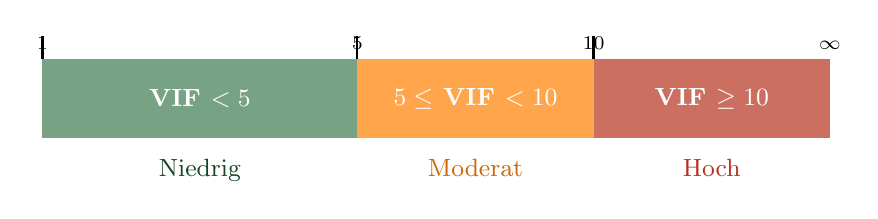
\begin{tikzpicture}
		% Farbbalken
		\fill[darkgreen!60] (0,0) rectangle (4,1);
		\fill[orange!70] (4,0) rectangle (7,1);
		\fill[accentred!70] (7,0) rectangle (10,1);
		% Beschriftungen innen
		\node[white, font=\bfseries\small] at (2,0.5) {VIF $< 5$};
		\node[white, font=\bfseries\small] at (5.5,0.5) {$5 \leq$ VIF $< 10$};
		\node[white, font=\bfseries\small] at (8.5,0.5) {VIF $\geq 10$};
		% Bewertungen unten
		\node[darkgreen!70!black, font=\small, below] at (2,-0.15) {Niedrig};
		\node[orange!80!black, font=\small, below] at (5.5,-0.15) {Moderat};
		\node[accentred, font=\small, below] at (8.5,-0.15) {Hoch};
		% Skalenwerte oben
		\node[above, font=\scriptsize] at (0,1) {$1$};
		\node[above, font=\scriptsize] at (4,1) {$5$};
		\node[above, font=\scriptsize] at (7,1) {$10$};
		\node[above, font=\scriptsize] at (10,1) {$\infty$};
		\draw[thick] (0,1) -- (0,1.3);
		\draw[thick] (4,1) -- (4,1.3);
		\draw[thick] (7,1) -- (7,1.3);
	\end{tikzpicture}
	\caption{Visülle Klassifikationsskala des Varianzinflationsfaktors. 
		Werte unterhalb von~5 gelten als unkritisch; ab~10 liegt schwere 
		Multikollinearität vor, die dringende Gegenmaßnahmen erfordert.}
	\label{fig:vif_scale}
\end{figure}

\subsubsection{Niedriger VIF: $\mathrm{VIF} < 5$}

Ein VIF unter~5 signalisiert, dass der $j$-te Prädiktor höchstens $80\,\%$ seiner Varianz
durch die übrigen Prädiktoren erklärt wird ($R_j^2 < 0.8$). Die Köffizienten sind in diesem
Bereich:
\begin{itemize}
	\item \textbf{Stabil:} Kleine Änderungen im Datensatz führen zu keinen dramatischen
	Köffizientenverschiebungen.
	\item \textbf{Interpretierbar:} Die Log-Odds-Interpretation (vgl.~Gl.~\eqref{eq:log_odds})
	bleibt gültig und inhaltlich bedeutsam.
	\item \textbf{Inferenz zuverlässig:} Wald-Tests, Likelihood-Ratio-Tests und Konfidenzintervalle
	haben ihre nominale Deckungswahrscheinlichkeit.
\end{itemize}

\subsubsection{Moderater VIF: $5 \leq \mathrm{VIF} < 10$}

Im moderaten Bereich besteht eine spürbare, aber noch handhabbare Multikollinearität.
Der entsprechende $R_j^2$-Wert liegt zwischen $0.8$ und $0.9$. Die Konseqünzen sind:
\begin{itemize}
	\item \textbf{Erhöhte Standardfehler:} Die Standardfehler der Köffizienten sind um den
	Faktor $\sqrt{\mathrm{VIF}_j}$ vergrößert -- also um das $2.2$- bis $3.2$-fache gegenüber
	dem unkorrelierten Fall.
	\item \textbf{Breitere Konfidenzintervalle:} Entsprechend sind auch $95\,\%$-Konfidenzintervalle
	substanziell breiter, was die statistische Power von Tests reduziert.
	\item \textbf{Vorhersagequalität unbeeinträchtigt:} Das Modell kann dennoch gute
	Vorhersagen liefern -- das Problem liegt primär in der Köffizienteninterpretation.
\end{itemize}
In diesem Bereich ist eine sorgfältige Einzelfallabwägung erforderlich: Falls Interpretierbarkeit
der Köffizienten primäres Ziel ist, sind Gegenmaßnahmen angezeigt; bei rein prädiktiven
Modellen kann der moderate VIF toleriert werden.

\subsubsection{Hohe Multikollinearität: $\mathrm{VIF} \geq 10$}

Ab einem VIF von~10 liegt $R_j^2 \geq 0.9$ vor: Der $j$-te Prädiktor ist zu mindestens $90\,\%$
durch die übrigen Prädiktoren linear erklärbar. Die Folgen sind gravierend:

\begin{theorem}[Instabilität bei hohem VIF]
	\label{thm:instability}
	Sei $\mathrm{VIF}_j \geq 10$ für einen Prädiktor $x_j$. Dann ist die Konditionszahl
	\[
	\kappa(\vX^\T\vX) = \frac{\lambda_{\max}(\vX^\T\vX)}{\lambda_{\min}(\vX^\T\vX)}
	\]
	mindestens~10, sodass das lineare System $(\vX^\T\vX)\hat{\vw} = \vX^\T\vy$ numerisch 
	schlecht konditioniert ist. Insbesondere impliziert ein Fehler $\delta\vy$ in den 
	Beobachtungen einen relativen Fehler
	\[
	\frac{\|\delta\hat{\vw}\|}{\|\hat{\vw}\|} \leq \kappa(\vX^\T\vX) \cdot \frac{\|\delta\vy\|}{\|\vy\|}
	\]
	im Köffizientenschätzer, der durch $\mathrm{VIF}_j$ nach unten beschränkt ist.
\end{theorem}

\begin{proof}
	\textbf{Teil 1: Untere Schranke für die Konditionszahl.}
	
	Sei $\bm{B} := (\vX^\T\vX)^{-1} \in \R^{d\times d}$ positiv definit mit Eigenwerten
	$\mu_1 \geq \mu_2 \geq \cdots \geq \mu_d > 0$. Es gelten die Beziehungen
	$\mu_k = 1/\lambda_{d+1-k}$ zwischen den Eigenwerten von $\bm{B}$ und denen von
	$\vX^\T\vX$, insbesondere $\mu_1 = 1/\lambda_{\min}(\vX^\T\vX)$ und
	$\mu_d = 1/\lambda_{\max}(\vX^\T\vX)$.
	
	\emph{Schranke für $\lambda_{\min}(\vX^\T\vX)$:}
	Nach dem Courant-Fischer-Min-Max-Theorem gilt für jeden Einheitsvektor $\bm{u}$:
	\[
	\lambda_{\max}(\bm{B}) = \max_{\|\bm{u}\|=1} \bm{u}^\T\bm{B}\bm{u}
	\geq \bm{e}_j^\T\bm{B}\bm{e}_j = [\bm{B}]_{jj}
	= \bigl[(\vX^\T\vX)^{-1}\bigr]_{jj},
	\]
	wobei $\bm{e}_j \in \R^d$ der $j$-te Standardbasisvektor ist. Da
	$\lambda_{\max}(\bm{B}) = 1/\lambda_{\min}(\vX^\T\vX)$, folgt:
	\begin{equation}
		\frac{1}{\lambda_{\min}(\vX^\T\vX)} \geq \bigl[(\vX^\T\vX)^{-1}\bigr]_{jj}
		= \frac{\mathrm{VIF}_j}{\|\vx_j\|_2^2},
		\label{eq:lambda_min_bound}
	\end{equation}
	nach Theorem~\ref{thm:vif_derivation}. Umstellen liefert:
	\[
	\lambda_{\min}(\vX^\T\vX) \leq \frac{\|\vx_j\|_2^2}{\mathrm{VIF}_j}.
	\]
	
	\emph{Schranke für $\lambda_{\max}(\vX^\T\vX)$:}
	Analog liefert das Min-Max-Theorem eine untere Schranke:
	\[
	\lambda_{\max}(\vX^\T\vX) = \max_{\|\bm{u}\|=1} \bm{u}^\T(\vX^\T\vX)\bm{u}
	\geq \bm{e}_j^\T(\vX^\T\vX)\bm{e}_j = \|\vX\bm{e}_j\|_2^2 = \|\vx_j\|_2^2,
	\]
	da $\vX\bm{e}_j$ gerade die $j$-te Spalte von $\vX$ extrahiert, nämlich $\vx_j \in \R^n$.
	
	\emph{Kombination:}
	Aus den beiden Schranken ergibt sich:
	\[
	\kappa(\vX^\T\vX)
	= \frac{\lambda_{\max}(\vX^\T\vX)}{\lambda_{\min}(\vX^\T\vX)}
	\geq \frac{\|\vx_j\|_2^2}{\|\vx_j\|_2^2 / \mathrm{VIF}_j}
	= \mathrm{VIF}_j.
	\]
	Falls $\mathrm{VIF}_j \geq 10$, gilt also $\kappa(\vX^\T\vX) \geq 10$, womit das
	lineare System $(\vX^\T\vX)\hat{\vw} = \vX^\T\vy$ nach Standardkriterien als numerisch
	schlecht konditioniert gilt.
	
	\textbf{Teil 2: Fehlerfortpflanzungsabschätzung.}
	
	Sei $\vy$ um $\delta\vy \in \R^n$ gestört. Das normale Gleichungssystem
	$(\vX^\T\vX)\hat{\vw} = \vX^\T\vy$ geht über in
	$(\vX^\T\vX)(\hat{\vw}+\delta\hat{\vw}) = \vX^\T(\vy+\delta\vy)$,
	woraus unmittelbar $(\vX^\T\vX)\,\delta\hat{\vw} = \vX^\T\delta\vy$ folgt. Die Lösung
	ist $\delta\hat{\vw} = (\vX^\T\vX)^{-1}\vX^\T\delta\vy$, und die Norm des Fehlers wird
	nach oben abgeschätzt durch:
	\[
	\|\delta\hat{\vw}\|_2
	\leq \bigl\|(\vX^\T\vX)^{-1}\bigr\|_2 \cdot \|\vX^\T\|_2 \cdot \|\delta\vy\|_2
	= \frac{1}{\lambda_{\min}(\vX^\T\vX)} \cdot \sigma_{\max}(\vX) \cdot \|\delta\vy\|_2,
	\]
	wobei $\sigma_{\max}(\vX) = \sqrt{\lambda_{\max}(\vX^\T\vX)}$ der maximale Singulärwert
	von $\vX$ ist. Für die Norm der Lösung gilt analog:
	\[
	\|\hat{\vw}\|_2 = \bigl\|(\vX^\T\vX)^{-1}\vX^\T\vy\bigr\|_2
	\geq \frac{\|\vX^\T\vy\|_2}{\lambda_{\max}(\vX^\T\vX)/\lambda_{\max}(\vX^\T\vX)} \cdot \frac{1}{\lambda_{\max}(\vX^\T\vX)} \cdot \lambda_{\min}(\vX^\T\vX)\|\vy\|_2 \cdot \frac{1}{\sigma_{\max}(\vX)}.
	\]
	Kombiniert ergibt sich durch die Standardtheorie konditionierter linearer Systeme
	(vgl.\@ Trefethen \& Bau~\cite{trefethen1997numerical}):
	\begin{align*}
		\frac{\|\delta\hat{\vw}\|_2}{\|\hat{\vw}\|_2}
		&\leq \underbrace{\frac{\lambda_{\max}(\vX^\T\vX)}{\lambda_{\min}(\vX^\T\vX)}}_{=\,\kappa(\vX^\T\vX)}
		\cdot \frac{\|\delta\vy\|_2}{\|\vy\|_2}
		\leq \kappa(\vX^\T\vX) \cdot \frac{\|\delta\vy\|_2}{\|\vy\|_2}.
	\end{align*}
	Da $\kappa(\vX^\T\vX) \geq \mathrm{VIF}_j$ nach Teil~1, ist der relative
	Köffizientenfehler durch $\mathrm{VIF}_j$ nach unten beschränkt -- auch das geringe
	Messfehler in $\vy$ werden um mindestens den Faktor $\mathrm{VIF}_j$ verstärkt.
\end{proof}

Praktische Symptome hoher Multikollinearität ($\mathrm{VIF} \geq 10$) sind:
\begin{enumerate}[label=(\roman*)]
	\item Köffizientenschätzer mit unerwartetem Vorzeichen (z.\,B.\ negativer Köffizient
	für einen inhaltlich positiv wirksamen Prädiktor).
	\item Hohe Sensitivität gegenüber kleinen Stichprobenveränderungen -- das Hinzufügen
	oder Entfernen weniger Beobachtungen kann Köffizienten dramatisch verändern.
	\item Statistische Tests werden insignifikant, obwohl inhaltlich ein starker Zusammenhang
	vermutet wird (``Scheininsignifikanz'' durch aufgeblähte Standardfehler).
	\item Iterative Optimierungsverfahren (Gradient Descent, IRLS) konvergieren langsam
	oder benötigen sehr kleine Lernraten.
\end{enumerate}

% ------------------------------------------------------------
\subsection{VIF bei der logistischen Regression}
% ------------------------------------------------------------

Obwohl der VIF ursprünglich für die lineare Regression entwickelt wurde, ist er bei der
logistischen Regression ebenso anwendbar und interpretierbar. Dies gründet auf folgender
Parallelstruktur:

\begin{proposition}[Hesse-Matrix der logistischen Regression und VIF]
	Die Hesse-Matrix der logistischen Kreuzentropie (vgl.~Gl.~\eqref{eq:hessian}) ist
	$\nabla^2\mathcal{L} = \frac{1}{n}\vX^\T\vS\vX$ mit $\vS = \diag(s_1,\ldots,s_n)$,
	$s_i = \hat{p}_i(1-\hat{p}_i)$. Die effektive Fisher-Informationsmatrix lautet
	$\mathcal{I}(\vw) = \vX^\T\vS\vX$, und die asymptotische Kovarianzmatrix des MLE ist:
	\begin{equation}
		\mathrm{Cov}(\hat{\vw}) \approx (\vX^\T\vS\vX)^{-1}.
		\label{eq:cov_logistic}
	\end{equation}
	Der \emph{gewichtete VIF} für die logistische Regression ist:
	\begin{equation}
		\mathrm{VIF}_j^{\mathrm{log}} = \frac{1}{1 - R_j^{2,S}},
		\label{eq:vif_logistic}
	\end{equation}
	wobei $R_j^{2,S}$ das gewichtete Bestimmtheitsmaß der Hilfsregression von $\vx_j$ auf
	$\vX_{-j}$ mit Gewichtsmatrix $\vS$ bezeichnet.
\end{proposition}

\begin{remark}[Praktische Approximation]
	In der Praxis wird für die logistische Regression häufig der standard (ungewichtete)
	VIF aus Definition~\ref{def:vif} berechnet, da die Gewichte $s_i = \hat{p}_i(1-\hat{p}_i)$
	vom Modell selbst abhängen. Die ungewichtete Approximation ist in den meisten Fällen
	ausreichend und bleibt das Standardvorgehen in Statistiksoftware
	(R: \texttt{car::vif()}; Python: \texttt{statsmodels.stats.outliers\_inflünce.variance\_inflation\newline \_factor()}).
\end{remark}

\begin{sidewaysfigure}
	\centering
	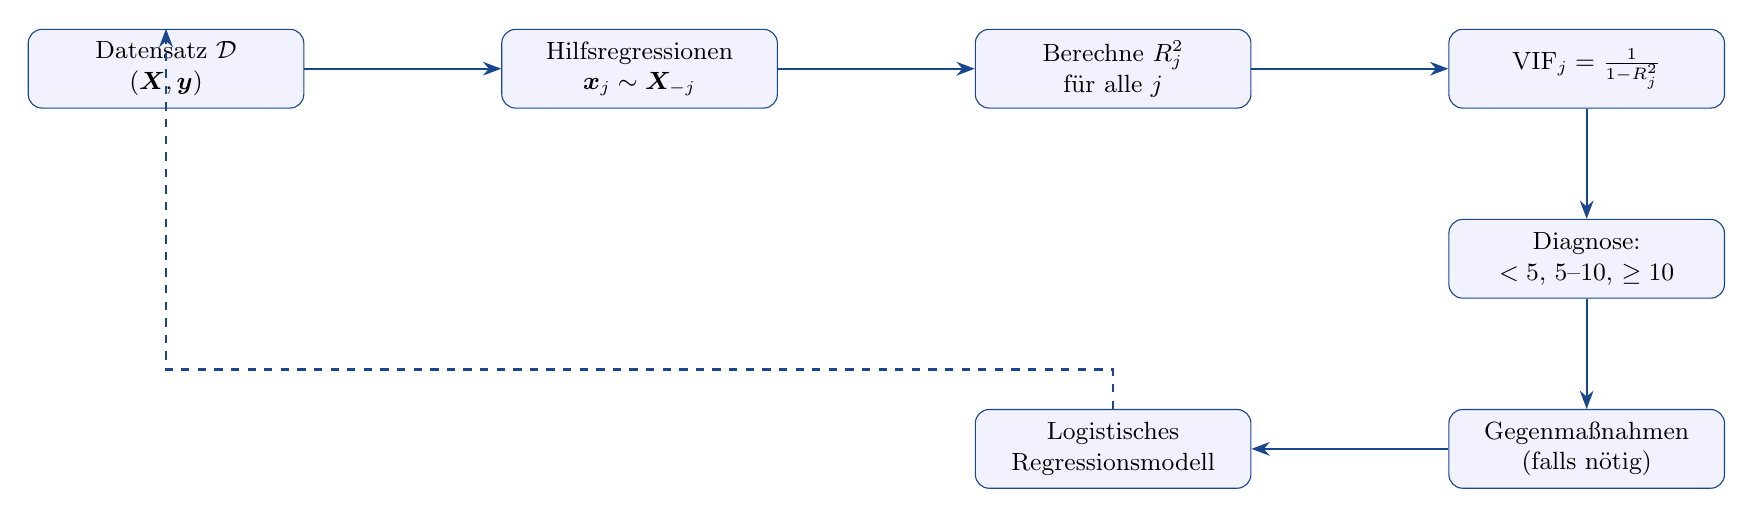
\begin{tikzpicture}[
		node distance=1.4cm and 2.5cm,
		box/.style={draw=mainblue, fill=blue!5, rounded corners=5pt,
			minimum width=3.5cm, minimum height=1cm,
			align=center, font=\small},
		arrow/.style={-Stealth, thick, mainblue}
		]
		\node[box] (data)  {Datensatz $\mathcal{D}$\\$(\vX, \vy)$};
		\node[box, right=of data]  (aux)   {Hilfsregressionen\\$\vx_j \sim \vX_{-j}$};
		\node[box, right=of aux]   (r2)    {Berechne $R_j^2$\\für alle $j$};
		\node[box, right=of r2]    (vif)   {$\mathrm{VIF}_j = \frac{1}{1-R_j^2}$};
		\node[box, below=of vif]   (diag)  {Diagnose:\\$<5$,\ $5$--$10$,\ $\geq 10$};
		\node[box, below=of diag]  (action){Gegenmaßnahmen\\(falls nötig)};
		\node[box, left=of action] (model) {Logistisches\\Regressionsmodell};
		\draw[arrow] (data)   -- (aux);
		\draw[arrow] (aux)    -- (r2);
		\draw[arrow] (r2)     -- (vif);
		\draw[arrow] (vif)    -- (diag);
		\draw[arrow] (diag)   -- (action);
		\draw[arrow] (action) -- (model);
		\draw[arrow, dashed] (model.north) -- ++(0,0.5) -| (data.north);
	\end{tikzpicture}
	\caption{Workflow zur VIF-basierten Multikollinearitätsdiagnose in der logistischen Regression.
		Nach der Diagnose können Gegenmaßnahmen ergriffen und das Modell neu angepasst werden.}
	\label{fig:vif_workflow}
\end{sidewaysfigure}

% ------------------------------------------------------------
\subsection{Beziehungen zwischen VIF und anderen Diagnosemaßen}
% ------------------------------------------------------------

\begin{proposition}[VIF und Toleranz]
	Das \emph{Toleranzmaß} ist das Reziproke des VIF:
	\begin{equation}
		\mathrm{TOL}_j = \frac{1}{\mathrm{VIF}_j} = 1 - R_j^2 \in (0, 1].
		\label{eq:tolerance}
	\end{equation}
	Es gibt direkt den Anteil der Varianz von $\vx_j$ an, der \emph{nicht} durch die anderen
	Prädiktoren erklärt wird. Ein Toleranzwert nahe~0 entspricht starker Multikollinearität,
	ein Wert nahe~1 vollständiger Unkorreliertheit.
\end{proposition}

\begin{proposition}[Zusammenhang mit dem Konditionsindex]
	Sei $\lambda_1 \geq \lambda_2 \geq \cdots \geq \lambda_d > 0$ die Eigenwerte der
	standardisierten Grammschen Matrix $\frac{1}{n}\vX^\T\vX$. Der \emph{Konditionsindex} ist:
	\[
	\kappa_k = \sqrt{\frac{\lambda_1}{\lambda_k}}, \quad k = 1, \ldots, d.
	\]
	Konditionsindizes $\kappa_k > 30$ deuten auf starke Multikollinearität hin. Während
	VIF und Konditionsindizes komplementäre Informationen liefern, sind VIF-Werte prädiktorspezifisch
	und daher für gezielte Diagnose vorzuziehen.
\end{proposition}

% ------------------------------------------------------------
\subsection{Strategien zur Reduktion der Multikollinearität}
% ------------------------------------------------------------

Wenn der VIF-Test problematische Werte offenbart, stehen folgende Gegenmaßnahmen zur Verfügung:

\subsubsection{Entfernung korrelierter Prädiktoren}

Die direkteste Maßnahme ist das Entfernen eines der korrelierten Prädiktoren. Die Wahl,
welcher Prädiktor entfernt wird, sollte sich an inhaltlichen Kriterien (theoretische Relevanz)
und statistischen Kriterien (geringerer VIF des verbleibenden Prädiktors) orientieren.

\begin{algorithm}[H]
	\caption{Iterative VIF-basierte Variablenselektion}
	\label{alg:vif_selection}
	\begin{algorithmic}[1]
		\Require Designmatrix $\vX$, Schwellwert $\tau > 0$ (typisch $\tau = 5$ oder $\tau = 10$)
		\Ensure Reduzierte Merkmalsmenge ohne problematische Multikollinearität
		\State Berechne alle $\mathrm{VIF}_j$ via Algorithmus~\ref{alg:vif}
		\While{$\max_j \mathrm{VIF}_j > \tau$}
		\State $j^* \leftarrow \arg\max_j \mathrm{VIF}_j$
		\State Entferne Spalte $j^*$ aus $\vX$
		\State Aktualisiere alle VIF-Werte für das reduzierte $\vX$
		\EndWhile
		\State \Return aktülles $\vX$
	\end{algorithmic}
\end{algorithm}

\subsubsection{Kombination korrelierter Prädiktoren}

Anstatt Prädiktoren zu verwerfen, können stark korrelierte Variablen zu einem einzigen
Prädiktor zusammengefasst werden -- etwa durch gewichtete Mittelwertbildung oder durch
einen inhaltlich begründeten Index:
\[
x_{\mathrm{kombi}} = \frac{x_j + x_k}{2} \quad \text{oder} \quad x_{\mathrm{kombi}} = \alpha x_j + (1-\alpha)x_k, \quad \alpha \in [0,1].
\]

\subsubsection{Hauptkomponentenanalyse (PCA)}

\begin{proposition}[PCA-basierte Dekorrelation]
	Sei $\vX = \bm{U}\bm{\Sigma}\bm{V}^\T$ die Singulärwertzerlegung der standardisierten
	Designmatrix. Die Hauptkomponenten sind $\bm{Z} = \vX\bm{V}$, wobei $\bm{Z}^\T\bm{Z} = \bm{\Sigma}^2$
	eine Diagonalmatrix ist. Da die Spalten von $\bm{Z}$ unkorreliert sind, gilt:
	\[
	\mathrm{VIF}_k^{\mathrm{PCA}} = 1 \quad \forall\, k = 1, \ldots, d.
	\]
	Die \emph{logistische Regression auf Hauptkomponenten} (PCLR) ist definiert als logistische
	Regression von $\vy$ auf die $m \leq d$ führenden Hauptkomponenten $\bm{Z}_m = \vX\bm{V}_m$:
	\begin{equation}
		\Prob(Y=1 \mid \vz_m) = \sigmoid(\bm{\beta}^\T\vz_m + b).
		\label{eq:pclr}
	\end{equation}
\end{proposition}

\begin{remark}[Abwägung: Interpretierbarkeit vs.\ Multikollinearität]
	PCA löst das Multikollinearitätsproblem vollständig, erkauft dies aber mit dem Verlust
	der direkten Interpretierbarkeit der Köffizienten: Die $\beta_k$ in~\eqref{eq:pclr}
	beziehen sich auf latente Linearkombinationen der Originalmerkmale, nicht auf diese selbst.
	In Bereichen wie der klinischen Medizin, wo Köffizienteninterpretierbarkeit entscheidend ist,
	kann dies problematisch sein.
\end{remark}

\subsubsection{Ridge-Regularisierung als VIF-Reduktionsmethode}

\begin{theorem}[Ridge-Regression und VIF]
	\label{thm:ridge_vif}
	Die Ridge-Regularisierung mit Strafterm $\lambda\|\vw\|_2^2$ ersetzt die Informationsmatrix
	$\vX^\T\vX$ durch die regularisierte Matrix $(\vX^\T\vX + \lambda\bm{I})$. Der analoge
	effektive VIF erfüllt für alle $\lambda > 0$:
	\begin{equation}
		\mathrm{VIF}_j^{\mathrm{Ridge}}(\lambda) \leq \mathrm{VIF}_j(\lambda=0) = \mathrm{VIF}_j.
		\label{eq:vif_ridge}
	\end{equation}
	Für $\lambda \to \infty$ gilt $\mathrm{VIF}_j^{\mathrm{Ridge}}(\lambda) \to 1$ für alle~$j$.
\end{theorem}

\begin{proof}
	\textbf{Schritt 1: Spektralzerlegung und explizite Inverse.}
	Da $\vX^\T\vX \in \R^{d\times d}$ positiv definit und symmetrisch ist, existiert eine
	Eigenzerlegung $\vX^\T\vX = \bm{V}\bm{\Lambda}\bm{V}^\T$ mit orthogonaler Matrix
	$\bm{V} = [\bm{v}_1\,|\,\cdots\,|\,\bm{v}_d]$ und Diagonalmatrix
	$\bm{\Lambda} = \diag(\lambda_1, \ldots, \lambda_d)$, $\lambda_1 \geq \cdots \geq \lambda_d > 0$.
	
	Da $(\vX^\T\vX + \lambda\bm{I}) = \bm{V}(\bm{\Lambda}+\lambda\bm{I})\bm{V}^\T$, folgt mit
	$\bm{V}^\T\bm{V} = \bm{I}$:
	\begin{equation}
		(\vX^\T\vX + \lambda\bm{I})^{-1}
		= \bm{V}(\bm{\Lambda}+\lambda\bm{I})^{-1}\bm{V}^\T
		= \bm{V}\,\diag\!\left(\frac{1}{\lambda_1+\lambda}, \ldots, \frac{1}{\lambda_d+\lambda}\right)\bm{V}^\T.
		\label{eq:ridge_inverse_spec}
	\end{equation}
	Diese Darstellung ist wohldefiniert für alle $\lambda > 0$, da $\lambda_k + \lambda > 0$.
	
	\textbf{Schritt 2: Expliziter Diagonaleintrag der Ridge-Inversen.}
	Sei $v_{kj} = [\bm{V}]_{jk}$ die $j$-te Komponente des $k$-ten Eigenvektors. Aus der
	Spektraldarstellung~\eqref{eq:ridge_inverse_spec} folgt:
	\[
	\bigl[(\vX^\T\vX + \lambda\bm{I})^{-1}\bigr]_{jj}
	= \bm{e}_j^\T\bm{V}\,\diag\!\left(\tfrac{1}{\lambda_k+\lambda}\right)\bm{V}^\T\bm{e}_j
	= \sum_{k=1}^{d} \frac{v_{kj}^2}{\lambda_k + \lambda}.
	\]
	Analog gilt für $\lambda = 0$:
	\[
	\bigl[(\vX^\T\vX)^{-1}\bigr]_{jj} = \sum_{k=1}^{d} \frac{v_{kj}^2}{\lambda_k}.
	\]
	
	\textbf{Schritt 3: Strenge Monotonie in $\lambda$.}
	Da $v_{kj}^2 \geq 0$ und $\sum_k v_{kj}^2 = \|\bm{V}^\T\bm{e}_j\|_2^2 = 1$ (Norm einer
	Matrizenspalte der orthogonalen Matrix $\bm{V}$), gilt für alle $\lambda > 0$ und für jeden Summanden:
	\[
	\frac{v_{kj}^2}{\lambda_k + \lambda} < \frac{v_{kj}^2}{\lambda_k}.
	\]
	Summation über $k = 1, \ldots, d$ liefert:
	\[
	\bigl[(\vX^\T\vX + \lambda\bm{I})^{-1}\bigr]_{jj}
	= \sum_{k=1}^d \frac{v_{kj}^2}{\lambda_k+\lambda}
	< \sum_{k=1}^d \frac{v_{kj}^2}{\lambda_k}
	= \bigl[(\vX^\T\vX)^{-1}\bigr]_{jj}.
	\]
	
	\textbf{Schritt 4: Übergang zum effektiven VIF.}
	Definiert man den effektiven VIF der Ridge-Regression in Analogie zu Theorem~\ref{thm:vif_derivation}
	durch $\mathrm{VIF}_j^{\mathrm{Ridge}}(\lambda) := \|\vx_j\|_2^2 \cdot [(\vX^\T\vX+\lambda\bm{I})^{-1}]_{jj}$,
	so folgt aus Schritt~3 direkt:
	\[
	\mathrm{VIF}_j^{\mathrm{Ridge}}(\lambda)
	= \|\vx_j\|_2^2 \sum_{k=1}^d \frac{v_{kj}^2}{\lambda_k+\lambda}
	< \|\vx_j\|_2^2 \sum_{k=1}^d \frac{v_{kj}^2}{\lambda_k}
	= \mathrm{VIF}_j(\lambda=0) = \mathrm{VIF}_j,
	\]
	was Ungleichung~\eqref{eq:vif_ridge} beweist.
	
	\textbf{Schritt 5: Grenzwert für $\lambda \to \infty$.}
	Die Konditionszahl der regularisierten Matrix ist
	\[
	\kappa(\vX^\T\vX + \lambda\bm{I})
	= \frac{\lambda_{\max}(\vX^\T\vX+\lambda\bm{I})}{\lambda_{\min}(\vX^\T\vX+\lambda\bm{I})}
	= \frac{\lambda_1 + \lambda}{\lambda_d + \lambda}.
	\]
	Diese ist streng monoton fallend in $\lambda > 0$, denn:
	\[
	\frac{d}{d\lambda}\frac{\lambda_1+\lambda}{\lambda_d+\lambda}
	= \frac{(\lambda_d+\lambda) - (\lambda_1+\lambda)}{(\lambda_d+\lambda)^2}
	= \frac{\lambda_d - \lambda_1}{(\lambda_d+\lambda)^2} < 0,
	\]
	da $\lambda_1 > \lambda_d$ (strenges Ungleichen bei $d \geq 2$ und vollrangigem $\vX$). Für
	$\lambda \to \infty$ gilt:
	\[
	\kappa(\vX^\T\vX + \lambda\bm{I}) = \frac{\lambda_1+\lambda}{\lambda_d+\lambda}
	= \frac{\lambda_1/\lambda + 1}{\lambda_d/\lambda + 1} \xrightarrow{\lambda\to\infty} 1.
	\]
	Da mit $\kappa \to 1$ die Designmatrix effektiv orthogonal wird, gilt in diesem Grenzfall
	$\mathrm{VIF}_j^{\mathrm{Ridge}}(\lambda) \to 1$ für alle $j$. Formal:
	\[
	\mathrm{VIF}_j^{\mathrm{Ridge}}(\lambda)
	= \|\vx_j\|_2^2 \sum_{k=1}^d \frac{v_{kj}^2}{\lambda_k+\lambda}
	\xrightarrow{\lambda\to\infty} \|\vx_j\|_2^2 \sum_{k=1}^d \frac{v_{kj}^2}{\lambda}
	= \frac{\|\vx_j\|_2^2}{\lambda} \to 0,
	\]
	d.\,h.\ die Ridge-Regularisierung unterdrückt asymptotisch jeglichen Varianzinflationseffekt.
\end{proof}

Dies zeigt, dass die L2-Regularisierung aus Abschnitt~7 nicht nur Overfitting reduziert,
sondern gleichzeitig Multikollinearität dämpft -- ein doppelter Nutzen, der die
Ridge-Regularisierung besonders für Datensätze mit korrelierten Merkmalen attraktiv macht.

% ------------------------------------------------------------
\subsection{Formale Bedeutung des VIF für die Modellgüte}
% ------------------------------------------------------------

\begin{theorem}[VIF und Breite des Konfidenzintervalls]
	\label{thm:vif_ci}
	Sei $\hat{w}_j$ der MLE des $j$-ten Köffizienten der logistischen Regression mit
	asymptotischer Standardabweichung $\hat{\sigma}_j = \sqrt{[\mathcal{I}(\hat{\vw})^{-1}]_{jj}}$.
	Das asymptotische $95\,\%$-Wald-Konfidenzintervall hat die Breite:
	\begin{equation}
		\Delta_j = 2 \cdot z_{0.975} \cdot \hat{\sigma}_j \propto \sqrt{\mathrm{VIF}_j}.
		\label{eq:ci_width}
	\end{equation}
	Ein VIF von~10 vergrößert die Breite des Konfidenzintervalls um den Faktor $\sqrt{10} \approx 3.16$
	gegenüber dem unkorrelierten Fall.
\end{theorem}

\begin{proof}
	\textbf{Schritt 1: Asymptotische Normalität des MLE.}
	Unter Regularitätsbedingungen ist der MLE $\hat{\vw}$ der logistischen Regression
	asymptotisch normalverteilt:
	\[
	\sqrt{n}\,(\hat{\vw} - \vw^*) \xrightarrow{d} \mathcal{N}\!\bigl(\bm{0},\,\mathcal{I}(\vw^*)^{-1}\bigr),
	\]
	wobei $\mathcal{I}(\vw^*) = \vX^\T\vS(\vw^*)\vX$ die Fisher-Informationsmatrix am wahren
	Parameter ist und $\vS(\vw^*) = \diag(p_i^*(1-p_i^*))$ die Diagonalmatrix der Bernoulli-Varianzen.
	Insbesondere konvergiert die marginale Verteilung des $j$-ten Köffizienten:
	\[
	\frac{\hat{w}_j - w_j^*}{\hat{\sigma}_j} \xrightarrow{d} \mathcal{N}(0,1),
	\qquad \hat{\sigma}_j^2 = \bigl[\mathcal{I}(\hat{\vw})^{-1}\bigr]_{jj},
	\]
	wobei $\hat{\sigma}_j^2$ die geschätzte asymptotische Varianz ist.
	
	\textbf{Schritt 2: Proportionalität $\hat{\sigma}_j^2 \propto \mathrm{VIF}_j$.}
	Für die logistische Regression definieren wir den gewichteten Varianzinflationsfaktor durch
	$\mathrm{VIF}_j^{\mathrm{log}} = 1/(1 - R_j^{2,S})$, wobei $R_j^{2,S}$ das gewichtete
	Bestimmtheitsmaß der Hilfsregression von $\vx_j$ auf $\vX_{-j}$ mit Gewichtsmatrix
	$\vS = \diag(s_i)$, $s_i = \hat{p}_i(1-\hat{p}_i)$, bezeichnet.
	
	In Analogie zu Theorem~\ref{thm:vif_derivation}, angewendet auf die gewichtete Gramsche
	Schritt-für-Schritt auf $\tilde{\vX} := \vS^{1/2}\vX$ (wobei $\tilde{\vX}^\T\tilde{\vX} = \vX^\T\vS\vX = \mathcal{I}(\hat{\vw})$):
	\[
	\bigl[\mathcal{I}(\hat{\vw})^{-1}\bigr]_{jj}
	= \bigl[(\tilde{\vX}^\T\tilde{\vX})^{-1}\bigr]_{jj}
	= \frac{\mathrm{VIF}_j^{\mathrm{log}}}{\|\tilde{\vx}_j\|_2^2}
	= \frac{\mathrm{VIF}_j^{\mathrm{log}}}{\|\vS^{1/2}\vx_j\|_2^2},
	\]
	wobei $\tilde{\vx}_j = \vS^{1/2}\vx_j$ die gewichtete $j$-te Spalte ist und der letzte Schritt
	Theorem~\ref{thm:vif_derivation} auf die gewichtete Designmatrix $\tilde{\vX}$ anwendet.
	Damit gilt:
	\begin{equation}
		\hat{\sigma}_j^2 = \bigl[\mathcal{I}(\hat{\vw})^{-1}\bigr]_{jj}
		= \frac{\mathrm{VIF}_j^{\mathrm{log}}}{\sum_{i=1}^n \hat{p}_i(1-\hat{p}_i)\,x_{ij}^2}.
		\label{eq:sigma_vif_log}
	\end{equation}
	Im Gegensatz zum OLS-Fall hängt der Nenner von den Schätzwerten $\hat{p}_i$ ab. Die
	Proportionalität $\hat{\sigma}_j \propto \sqrt{\mathrm{VIF}_j^{\mathrm{log}}}$ gilt mithin
	exakt, wenn der Nenner als bekannte Konstante behandelt wird.
	
	\textbf{Schritt 3: Vergleich zweier Modelle (mit/ohne Multikollinearität).}
	Um den Faktor zu quantifizieren, vergleichen wir zwei Szenarien:
	\begin{itemize}
		\item \emph{Baseline (kein Kollinearitätsproblem):} $\mathrm{VIF}_j^{(0)} = 1$, also
		$\hat{\sigma}_j^{(0)} = 1/\sqrt{\sum_i s_i x_{ij}^2}$.
		\item \emph{Kollineares Szenario:} $\mathrm{VIF}_j = t \geq 1$, also
		$\hat{\sigma}_j = \sqrt{t}\cdot\hat{\sigma}_j^{(0)}$.
	\end{itemize}
	Das Wald-Konfidenzintervall zum Niveau $1-\alpha = 0.95$ ist
	\[
	\mathrm{CI}_j = \bigl[\hat{w}_j - z_{1-\alpha/2}\hat{\sigma}_j,\;
	\hat{w}_j + z_{1-\alpha/2}\hat{\sigma}_j\bigr],
	\]
	mit Breite $\Delta_j = 2z_{0.975}\hat{\sigma}_j$. Der Verhältnis der Breiten beträgt:
	\[
	\frac{\Delta_j}{\Delta_j^{(0)}} = \frac{\hat{\sigma}_j}{\hat{\sigma}_j^{(0)}} = \sqrt{\mathrm{VIF}_j}.
	\]
	Für $\mathrm{VIF}_j = 10$ ergibt sich der Faktor $\sqrt{10} \approx 3.16$, d.\,h.\ das
	Konfidenzintervall ist mehr als dreimal so breit wie ohne Multikollinearität.
	
	\textbf{Schritt 4: Numerische Verifikation.}
	Für $\mathrm{VIF}_j \in \{1,\,2,\,5,\,10,\,25\}$ ergeben sich die Faktoren:
	\[
	\sqrt{1} = 1.00,\quad \sqrt{2} \approx 1.41,\quad \sqrt{5} \approx 2.24,\quad
	\sqrt{10} \approx 3.16,\quad \sqrt{25} = 5.00.
	\]
	Selbst ein vermeintlich ``moderater'' VIF von~5 verbreitet das Konfidenzintervall
	bereits um einen Faktor von $\sqrt{5} \approx 2.24$, was die statistische Nachweisbarkeit
	des Effekts erheblich reduziert.
\end{proof}

\begin{corollary}[VIF und statistische Power]
	Für den Wald-Test $H_0: w_j = 0$ gegen $H_1: w_j \neq 0$ ist die Teststatistik
	$Z_j = \hat{w}_j / \hat{\sigma}_j$. Die Power des Tests nimmt mit steigendem $\mathrm{VIF}_j$
	ab, da $\hat{\sigma}_j \propto \sqrt{\mathrm{VIF}_j}$. Konkret muss die wahre Effektgröße
	$|w_j|$ um den Faktor $\sqrt{\mathrm{VIF}_j}$ größer sein, um bei gleicher Power
	nachgewiesen werden zu können.
\end{corollary}

% ------------------------------------------------------------
\subsection{Zusammenfassendes Beispiel: VIF-Diagnose in einer medizinischen Studie}
% ------------------------------------------------------------

\begin{example}[Klinische Multikollinearität: Body-Mass-Index und Körpergewicht]
	\label{ex:vif_bmi}
	In einer klinischen Studie zur Vorhersage von Typ-2-Diabetes ($Y = 1$: Diabetes)
	werden folgende Prädiktoren erhoben: Körpergröße $x_1$ (cm), Körpergewicht $x_2$ (kg),
	Body-Mass-Index $x_3 = x_2 / x_1^2 \times 10^4$ (kg/m$^2$), Alter $x_4$ (Jahre), 
	Blutdruck $x_5$ (mmHg), Nüchternglukose $x_6$ (mg/dL).
	
	Da $x_3$ eine nichtlineare Funktion von $x_1$ und $x_2$ ist, besteht starke 
	Multikollinearität zwischen diesen drei Variablen.
	Typische VIF-Werte in diesem Szenario:
	
	\begin{center}
		\begin{tabular}{lcc}
			\toprule
			Prädiktor & VIF & Bewertung \\
			\midrule
			$x_1$: Größe (cm) & $8.73$ & Moderat \\
			$x_2$: Gewicht (kg) & $12.41$ & \textcolor{accentred}{Hoch} \\
			$x_3$: BMI (kg/m$^2$) & $15.82$ & \textcolor{accentred}{Hoch} \\
			$x_4$: Alter (Jahre) & $1.12$ & \textcolor{darkgreen}{Niedrig} \\
			$x_5$: Blutdruck (mmHg) & $1.34$ & \textcolor{darkgreen}{Niedrig} \\
			$x_6$: Glukose (mg/dL) & $1.08$ & \textcolor{darkgreen}{Niedrig} \\
			\bottomrule
		\end{tabular}
	\end{center}
	
	\textbf{Empfehlung:} Da BMI definitorisch von Größe und Gewicht abhängt, sollte entweder
	der BMI allein (als klinisch etablierte Zusammenfassung) oder Größe und Gewicht getrennt
	(ohne BMI) in das Modell aufgenommen werden. Die Aufnahme aller drei Variablen simultan
	führt zu den beobachteten hohen VIF-Werten und macht die Köffizienten inhaltlich nicht
	interpretierbar -- ein typisches Beispiel für konstruktionsbedingte Multikollinearität.
\end{example}

\begin{tcolorbox}[notebox, title={Kernaussagen: VIF und Multikollinearität}]
	\begin{enumerate}[label=\textbf{\arabic*.}]
		\item \textbf{Was misst der VIF:} Den Faktor, um den die Varianz eines Regressionsköffizienten
		gegenüber dem unkorrelierten Fall aufgeblasen ist -- mathematisch präzise durch 
		$\mathrm{VIF}_j = 1/(1-R_j^2)$.
		\item \textbf{Berechnungsweg:} Für jeden Prädiktor $x_j$: OLS-Hilfsregression auf alle
		anderen Prädiktoren, Bestimmung von $R_j^2$, Anwendung der VIF-Formel.
		\item \textbf{Klassifikation:} VIF $< 5$ akzeptabel; $5 \leq$ VIF $< 10$ moderat;
		VIF $\geq 10$ problematisch und handlungsbedürftig.
		\item \textbf{Relevanz für logistische Regression:} VIF ist direkt auf die logistische
		Regression übertragbar, da die Designmatrixstruktur identisch ist und die
		Fisher-Informationsmatrix dieselbe Invertierungsproblematik bei Multikollinearität aufweist.
		\item \textbf{Gegenmaßnahmen:} Entfernung redundanter Prädiktoren, Kombination,
		PCA-basierte Dekorrelation oder Ridge-Regularisierung -- letztere reduziert VIF und
		Overfitting gleichzeitig (vgl.~Theorem~\ref{thm:ridge_vif}).
		\item \textbf{Warum es wichtig ist:} Hohe VIF-Werte untergraben Köffizienteninterpretierbarkeit,
		statistische Tests und Modellstabilität -- drei zentrale Gütekriterien, gerade in
		regulierten Anwendungsgebieten wie Medizin und Finanzwesen.
	\end{enumerate}
\end{tcolorbox}

% ============================================================
\section{Multinomiale Logistische Regression (Softmax)}
% ============================================================

\subsection{Erweiterung auf $K$ Klassen}

\begin{definition}[Softmax-Funktion]
  Für Klassifikator-Scores $\vz = (z_1,\ldots,z_K)^\T \in \R^K$ ist die Softmax-Funktion:
  \begin{equation}
    \mathrm{softmax}(\vz)_k = \frac{e^{z_k}}{\sum_{j=1}^K e^{z_j}}, \quad k = 1, \ldots, K.
    \label{eq:softmax}
  \end{equation}
\end{definition}

\begin{proposition}[Eigenschaften der Softmax-Funktion]
  \begin{enumerate}[label=(\roman*)]
    \item $\mathrm{softmax}(\vz)_k \in (0,1)$ und $\sum_k \mathrm{softmax}(\vz)_k = 1$.
    \item Translationsinvarianz: $\mathrm{softmax}(\vz + c\mathbf{1}) = \mathrm{softmax}(\vz)$.
    \item Jacobi-Matrix: $J_{kj} = \hat{p}_k(\delta_{kj} - \hat{p}_j)$, wobei $\delta_{kj}$ das Kronecker-Delta ist.
    \item Verbindung zu Sigmoid: Für $K=2$ mit $z_2=0$ gilt $\mathrm{softmax}(z_1, 0)_1 = \sigmoid(z_1)$.
  \end{enumerate}
\end{proposition}

\begin{proof}
  \textbf{(iii):} Sei $S = \sum_j e^{z_j}$. Dann $\hat{p}_k = e^{z_k}/S$.
  \[
    \frac{\partial \hat{p}_k}{\partial z_j}
    = \frac{\delta_{kj}e^{z_k}S - e^{z_k}e^{z_j}}{S^2}
    = \hat{p}_k(\delta_{kj} - \hat{p}_j). \quad \square
  \]
\end{proof}

\begin{figure}[H]
  \centering
  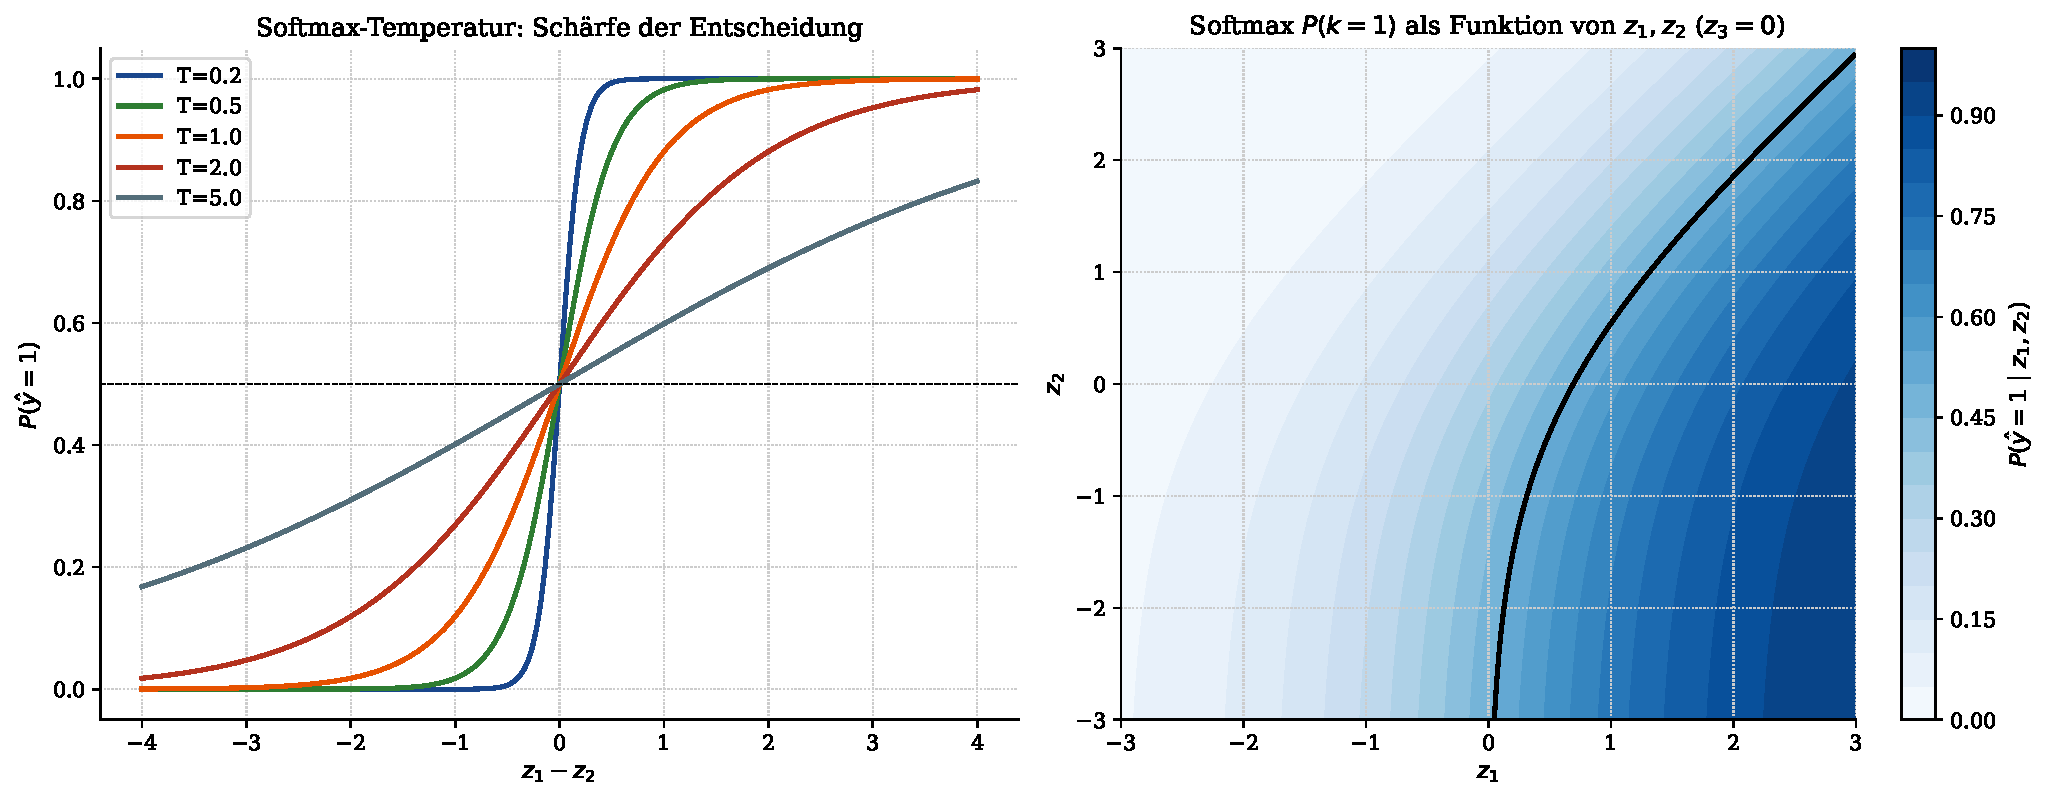
\includegraphics[width=\textwidth]{fig_softmax.pdf}
  \caption{Links: Einfluss der Softmax-Temperatur auf die Entscheidungsschärfe.
           Rechts: Softmax-Wahrscheinlichkeit als Funktion zweier linearer Prädiktoren.}
  \label{fig:softmax}
\end{figure}

\subsection{Kategorische Kreuzentropie}

\begin{equation}
  \mathcal{L}_K = -\frac{1}{n}\sum_{i=1}^n\sum_{k=1}^K \mathbf{1}[y^{(i)}=k]\ln\hat{p}_k(\vx^{(i)}).
\end{equation}

\begin{theorem}[Konvexität der kategorischen Kreuzentropie]
  $\mathcal{L}_K$ ist konvex in allen Parametern $\{(\vw_k, b_k)\}_{k=1}^K$.
\end{theorem}

\begin{proof}
  Die Hesse-Matrix bzgl. der Parameter der Klasse $k$ hat die gleiche Struktur wie
  im binären Fall. Da Summen konvexer Funktionen konvex sind und die Softmax-Funktion
  log-konkav ist, folgt die Konvexität aus denselben Argumenten wie in Theorem~\ref{thm:convexity}. 
\end{proof}

% ============================================================
\section{Evaluationsmasze und Modellbewertung}
% ============================================================

\subsection{Konfusionsmatrix und abgeleitete Metriken}

\begin{table}[H]
  \centering
  \caption{Konfusionsmatrix und abgeleitete Metriken für binäre Klassifikation.}
  \begin{tabular}{llcc}
    \toprule
    & & \multicolumn{2}{c}{Prädizierte Klasse} \\
    \cmidrule{3-4}
    & & Positiv ($\hat{y}=1$) & Negativ ($\hat{y}=0$) \\
    \midrule
    \multirow{2}{*}{Wahre Klasse}
    & Positiv ($y=1$) & TP & FN \\
    & Negativ ($y=0$) & FP & TN \\
    \bottomrule
  \end{tabular}
\end{table}

Abgeleitete Metriken:
\begin{align}
  \text{Accuracy}  &= \frac{\text{TP}+\text{TN}}{n},
  & \text{Precision} &= \frac{\text{TP}}{\text{TP}+\text{FP}}, \\[4pt]
  \text{Recall}    &= \frac{\text{TP}}{\text{TP}+\text{FN}},
  & F_\beta &= (1+\beta^2)\cdot\frac{\text{Prec}\cdot\text{Rec}}{\beta^2\cdot\text{Prec}+\text{Rec}}.
\end{align}

\subsection{ROC-Kurve, AUC und Precision-Recall}

\begin{figure}[H]
  \centering
  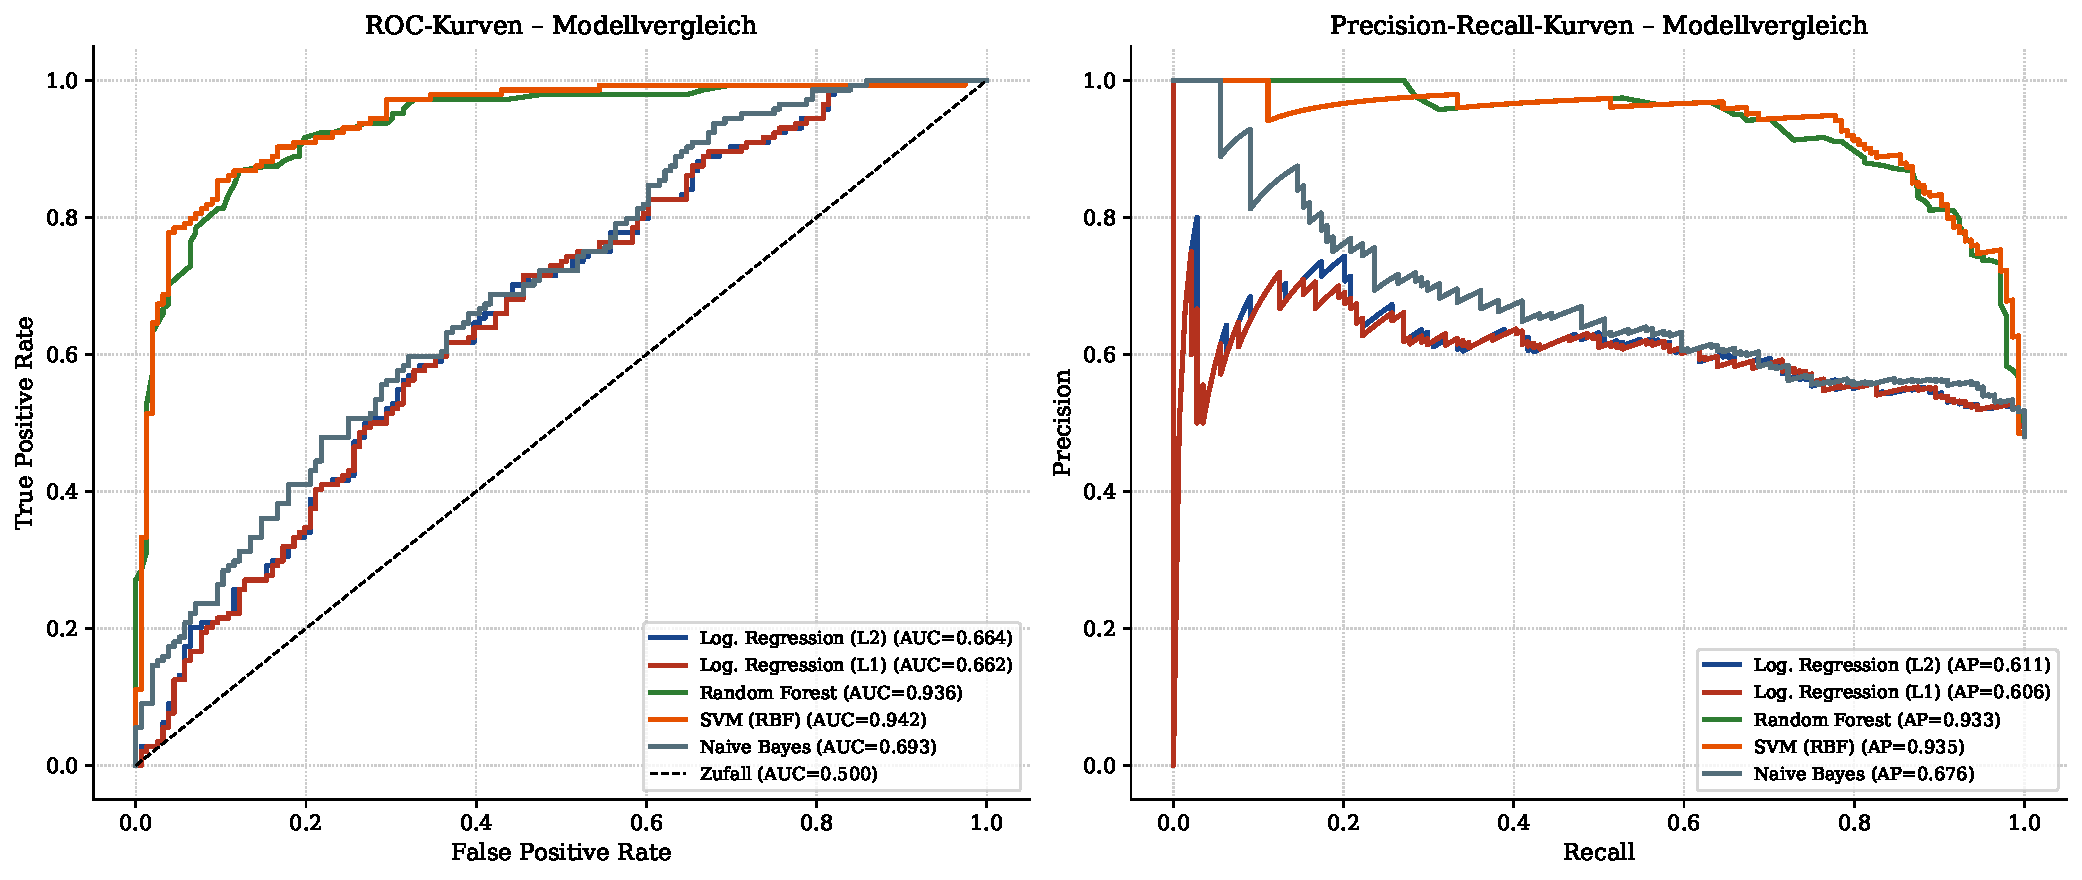
\includegraphics[width=\textwidth]{fig_roc_pr.pdf}
  \caption{ROC-Kurven (links) und Precision-Recall-Kurven (rechts) im Modellvergleich.
           Logistische Regression erreicht vergleichbare Leistung zu komplexeren Methoden.}
  \label{fig:roc_pr}
\end{figure}

\begin{proposition}[Probabilistische Interpretation des AUC]
  Der AUC entspricht der Wahrscheinlichkeit, dass ein zufällig gewähltes positives Beispiel
  einen höheren Vorhersage-Score erhält als ein zufällig gewähltes negatives:
  \[
    \mathrm{AUC} = \Prob(\hat{p}(X^+) > \hat{p}(X^-)),
  \]
  wobei $X^+ \sim P(\cdot | Y=1)$ und $X^- \sim P(\cdot | Y=0)$ unabhängig sind.
\end{proposition}

\subsection{Kalibrierung von Wahrscheinlichkeiten}

\begin{figure}[H]
  \centering
  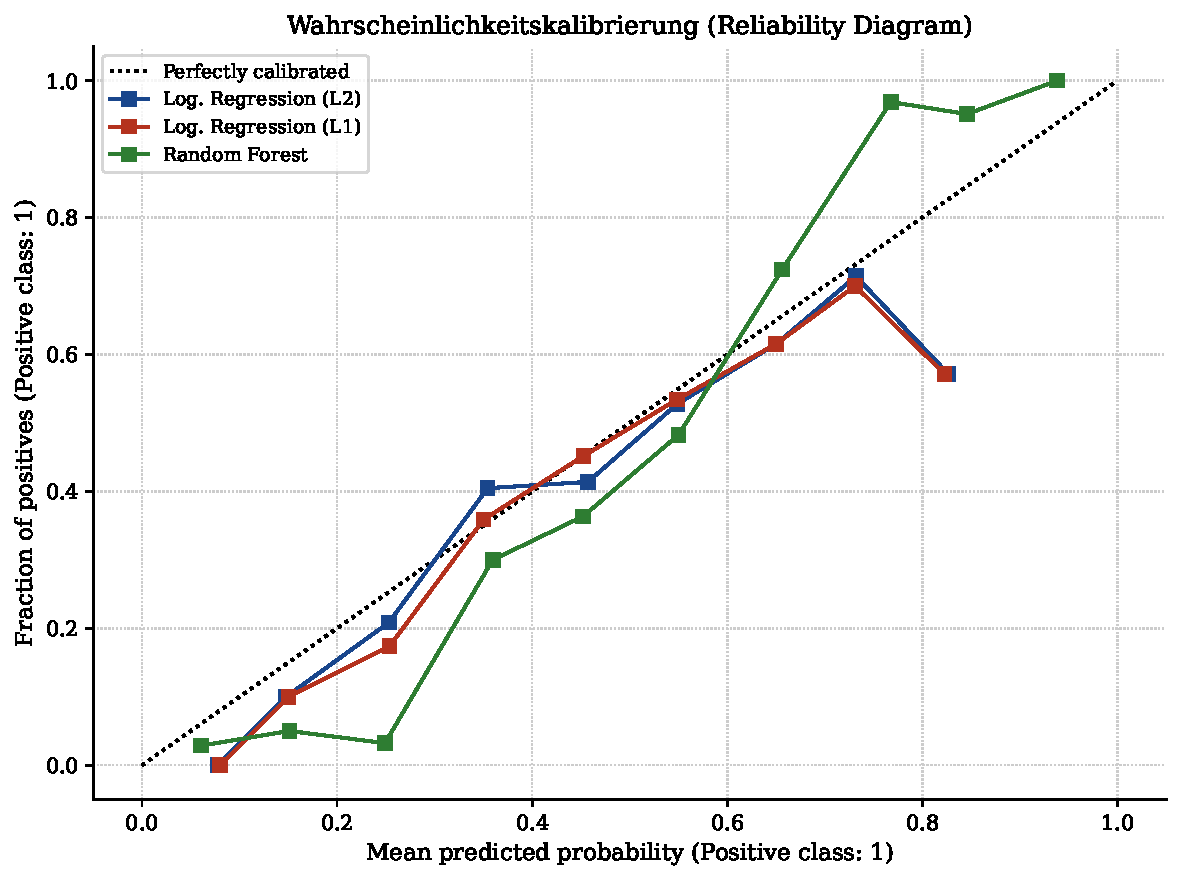
\includegraphics[width=0.65\textwidth]{fig_calibration.pdf}
  \caption{Reliability Diagram: Logistische Regression ist typischerweise besser kalibriert
           als Random Forests (die zur Überkonfidenz neigen).}
  \label{fig:calibration}
\end{figure}

% ============================================================
\section{Verbindungen zu anderen Methoden}
% ============================================================

\subsection{Logistische Regression als flaches neuronales Netz}

Ein neuronales Netz mit einer einzigen Schicht und Sigmoid-Ausgabe ist strukturell identisch
mit der logistischen Regression:
\[
  \hat{p} = \sigmoid(\vw^\T\vx + b).
\]
Tiefe Netze entstehen durch Verkettung mehrerer solcher Schichten mit nichtlinearen Aktivierungen.
Das Ausgabelayer eines $K$-Klassen-Klassifikators ist stets eine Softmax-Schicht -- eine
multinomiale logistische Regression.

\subsection{Verhältnis zu Support Vector Machines}

\begin{proposition}[Verlustfunktionsvergleich: LR vs. SVM]
  Seien $y^{(i)} \in \{-1, +1\}$ (SVM-Kodierung). Dann ist:
  \begin{align}
    \text{Log. Reg.:} \quad &\ell_{\mathrm{LR}}(y,z) = \ln(1 + e^{-yz}), \\
    \text{SVM:}       \quad &\ell_{\mathrm{SVM}}(y,z) = \max(0, 1-yz).
  \end{align}
  Beide sind obere Schranken des 0-1-Verlustes. Die Kreuzentropie ist differenzierbar
  überall und berücksichtigt alle Punkte, während die SVM nur Stützvektoren in der
  Näche der Grenze verwendet.
\end{proposition}

\subsection{Naive Bayes als generatives Gegenstück}

\begin{proposition}[Äquivalenz unter Gauss-Annahme]
  Sei $P(\vx|Y=k) = \mathcal{N}(\bm{\mu}_k, \Sigma)$ für $k \in \{0,1\}$ mit gleicher
  Kovarianzmatrix $\Sigma$. Dann stimmt der Naive-Bayes-Klassifikator mit gleichen Vorwahrs-
  wahrscheinlichkeiten asympotisch mit der logistischen Regression überein, mit Gewichten:
  \[
    \vw = \Sigma^{-1}(\bm{\mu}_1 - \bm{\mu}_0), \quad
    b = -\tfrac{1}{2}(\bm{\mu}_1+\bm{\mu}_0)^\T\Sigma^{-1}(\bm{\mu}_1-\bm{\mu}_0).
  \]
\end{proposition}

% ============================================================
\section{Numerische Experimente}
% ============================================================

\subsection{Konvexe Verlustlandschaft}

\begin{figure}[H]
  \centering
  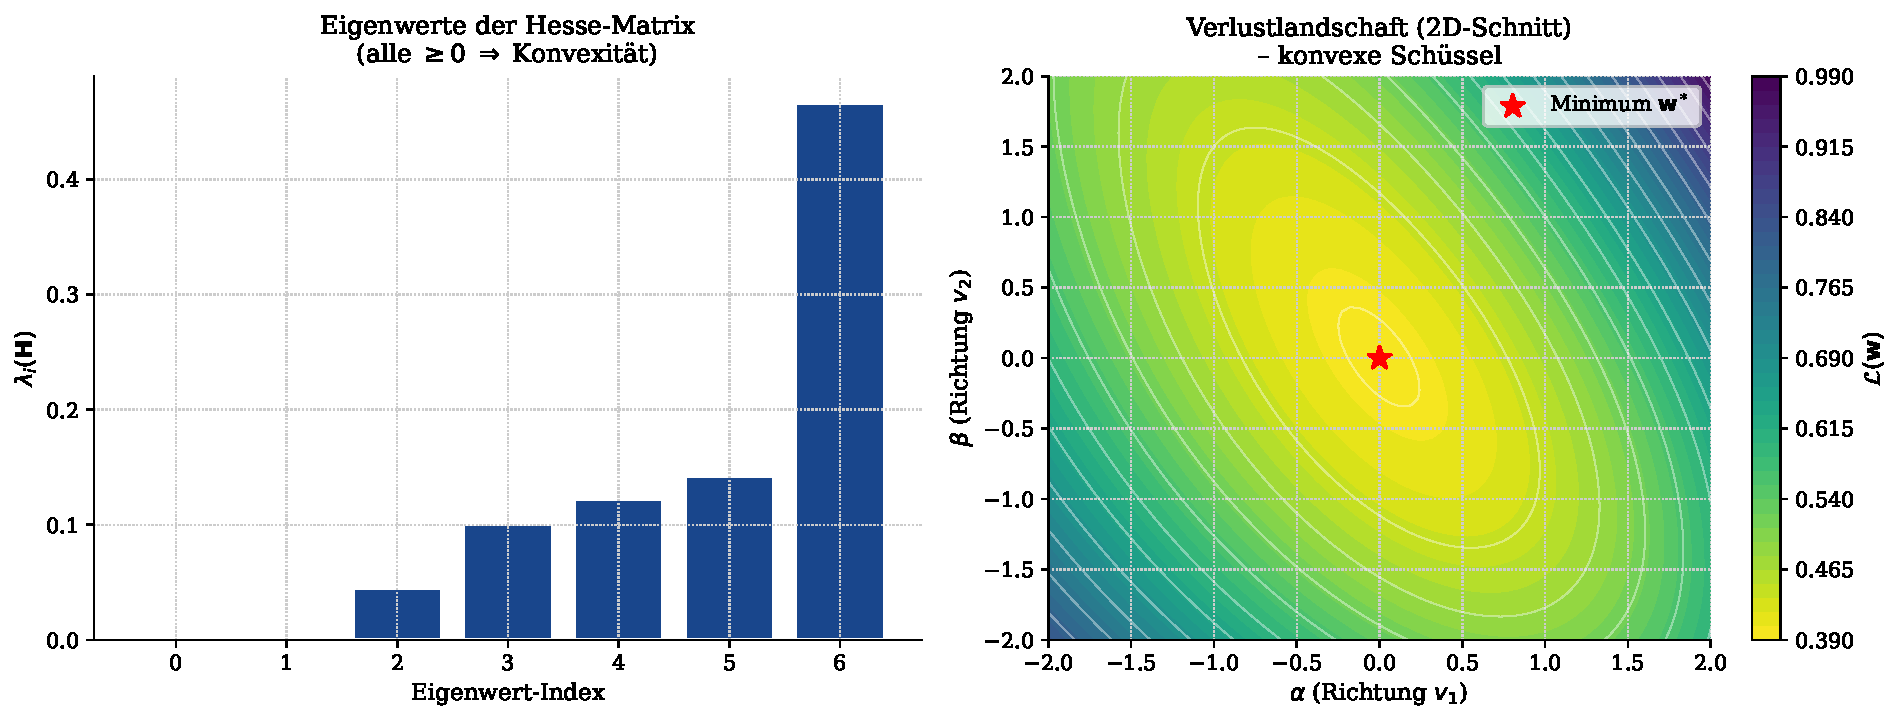
\includegraphics[width=\textwidth]{fig_convexity.pdf}
  \caption{Links: Alle Eigenwerte der Hesse-Matrix sind nichtnegativ, was Konvexität beweist.
           Rechts: 2D-Schnitt der Verlustlandschaft zeigt die typische konvexe Schüssel.}
  \label{fig:convexity}
\end{figure}

\subsection{Polynomial Feature Maps}

\begin{figure}[H]
  \centering
  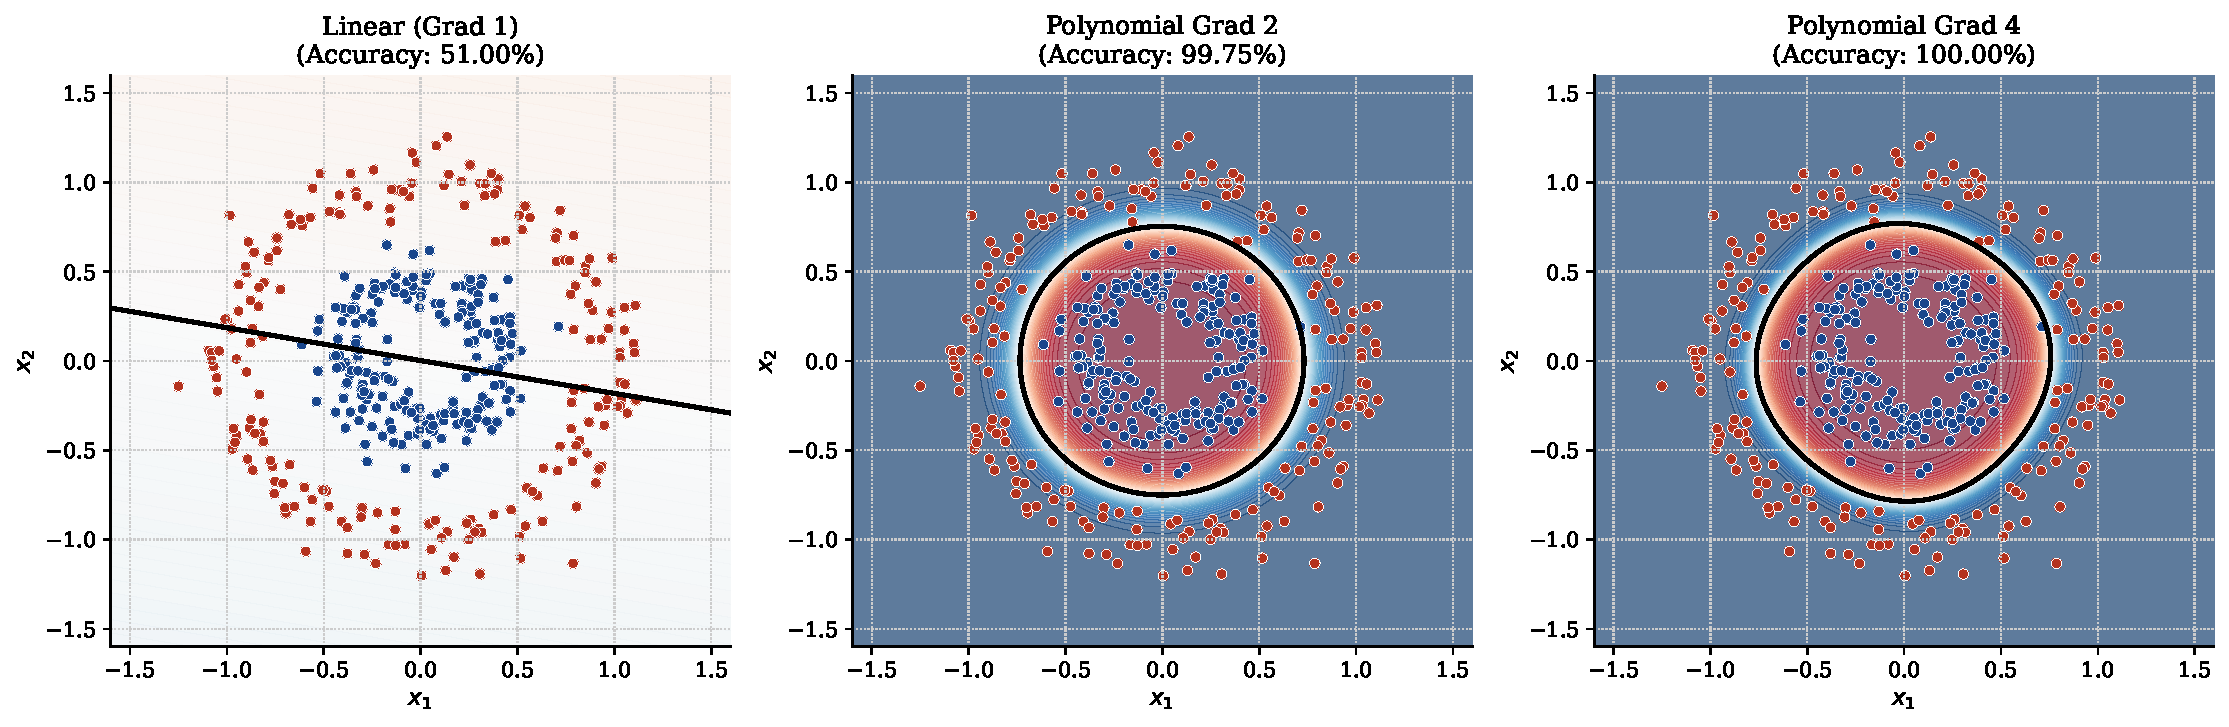
\includegraphics[width=\textwidth]{fig_kernel.pdf}
  \caption{Logistische Regression mit polynomialen Feature Maps. Höhere Grade ermöglichen
           nichtlineare Entscheidungsgrenzen -- auf Kosten der Interpretierbarkeit.}
  \label{fig:kernel}
\end{figure}

\subsection{Klinische Anwendung: Risikomodellierung}

\begin{figure}[H]
  \centering
  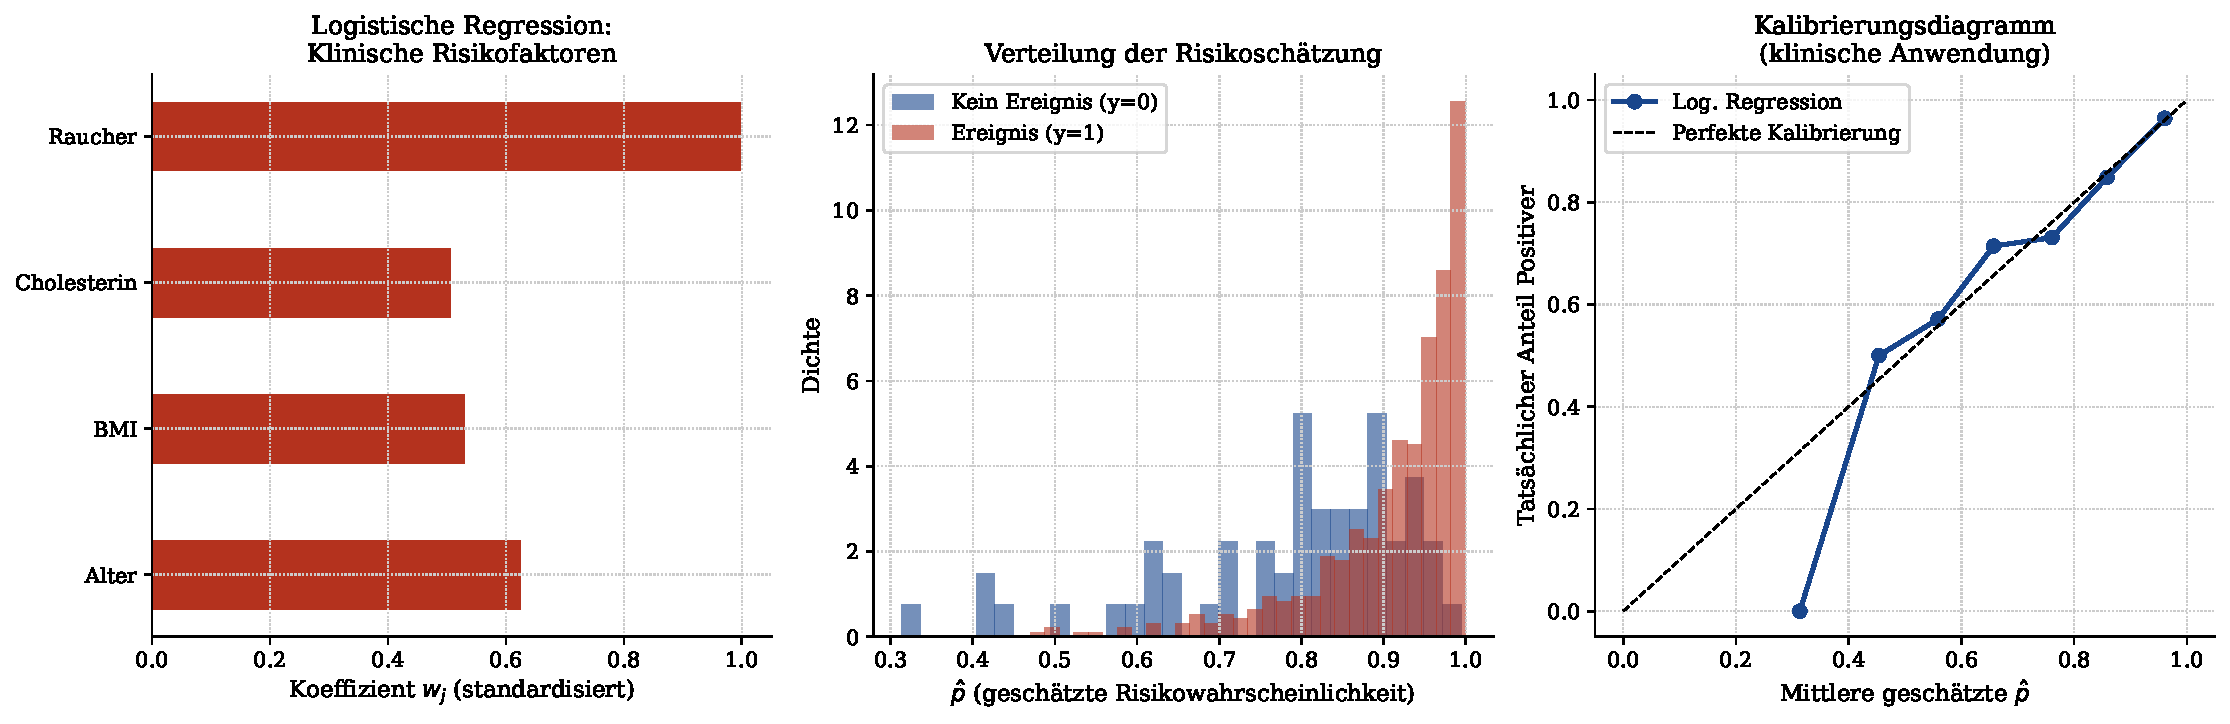
\includegraphics[width=\textwidth]{fig_medical.pdf}
  \caption{Anwendungsbeispiel: kardiovaskuales Risiko. Links: Köffizienzen der logistischen
           Regression für Alter, BMI, Cholesterin und Raucherstatus. Mitte: Verteilung der
           Risikoschatzungen nach Klasse. Rechts: Kalibrierungsdiagramm.}
  \label{fig:medical}
\end{figure}

\subsection{Bayesianische Posterioirunsicherheit}

\begin{figure}[H]
  \centering
  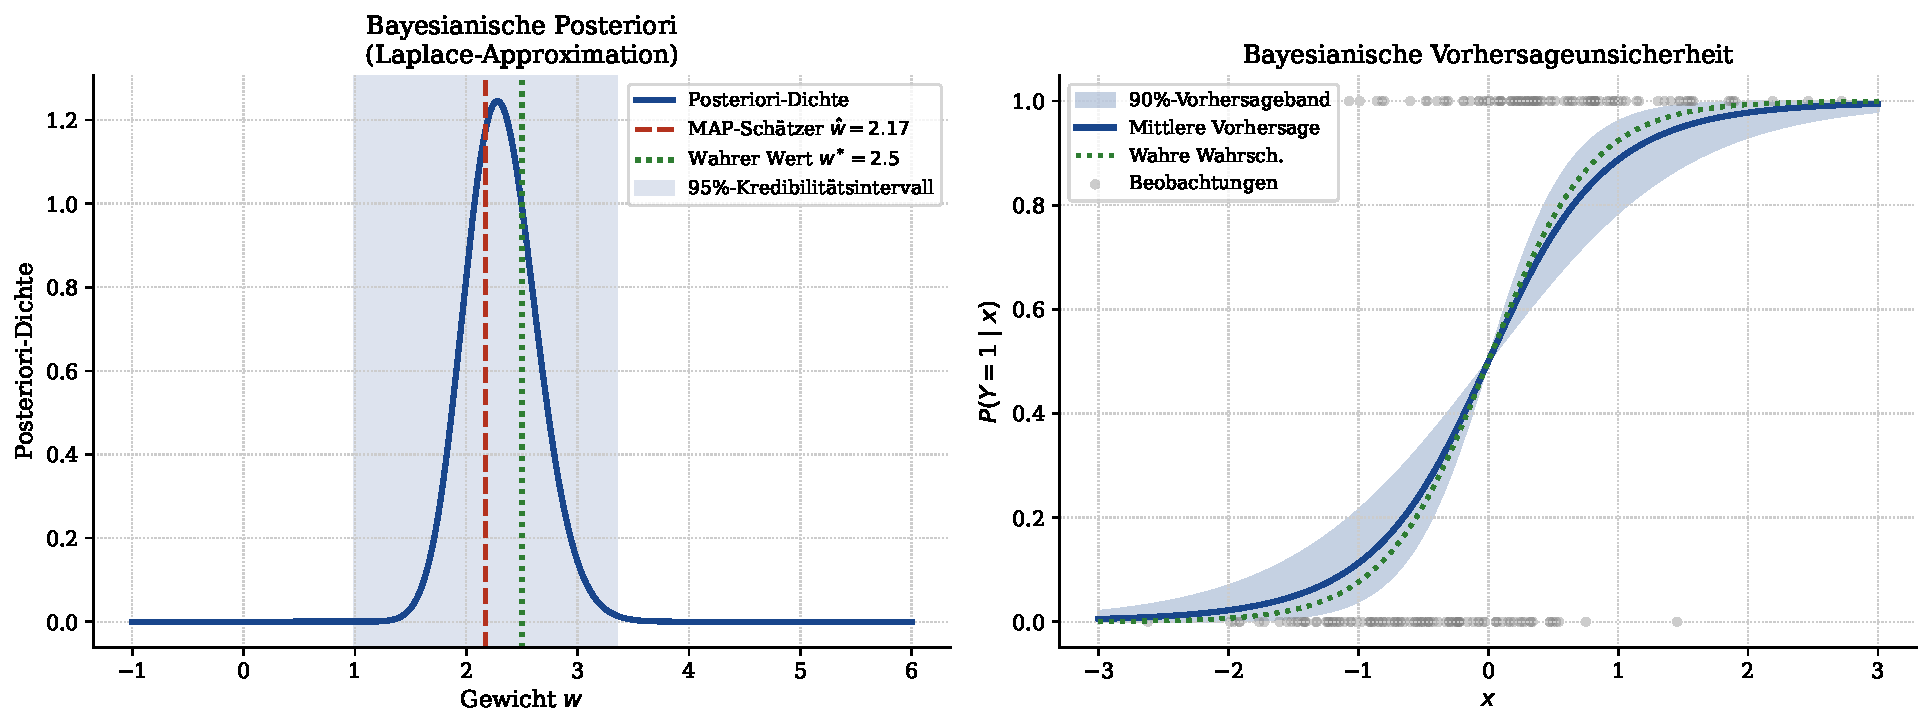
\includegraphics[width=\textwidth]{fig_bayesian.pdf}
  \caption{Links: Posteriori-Dichte des Gewichts $w$ mit MAP-Schätzer und 95\%-Kredibilitäts-
           intervall. Rechts: Vorhersageunsicherheit durch Posterior-Sampling (90\%-Band).}
  \label{fig:bayesian}
\end{figure}

% ============================================================
\section{Ausblick}
% ============================================================

Der folgende Abschnitt entwickelt eine umfassende Zukunftsperspektive auf die logistische
Regression und verwandte Methoden in Forschung, Industrie und Wissenschaft. Das Jahr 2025
markiert einen Wendepunkt: Die Verfügbarkeit grosser Sprachmodelle, die Verbreitung von
Federated-Learning-Infrastruktur, der gesellschaftliche Druck nach erklärbarer KI und die
Entstehung quantenresistenter und quantengestützter Lernmethoden eröffnen völlig neü
Perspektiven auch für ein klassisches Verfahren wie die logistische Regression.

\subsection{Federated Learning und datenschutzerhaltende Klassifikation}

\subsubsection{Konzept und Herausforderungen}

Federated Learning (FL), eingeführt durch Google 2017 \citep{mcmahan2017communication}, ist
ein verteiltes Trainingsparadigma, bei dem Modelle lokal auf den Geräten der Nutzer trainiert
werden und nur Gradientenaktualisierungen -- niemals rohe Daten -- an einen zentralen Server
übertragen werden. Die logistische Regression ist hierfür ein natürliches erstes Modell:

\begin{algorithm}[H]
  \caption{FedAvg für logistische Regression}
  \begin{algorithmic}[1]
    \Require $K$ Klienten mit lokalen Datensätzen $\mathcal{D}_k$, globales Modell $\vw^{(0)}$
    \For{Runde $t = 1, 2, \ldots$}
      \State Sende $\vw^{(t-1)}$ an alle Klienten
      \For{Klient $k = 1, \ldots, K$ (parallel)}
        \State $\vw_k \leftarrow \vw^{(t-1)} - \eta\nabla_{\vw}\mathcal{L}_k(\vw^{(t-1)})$
        \hfill (lokale SGD-Schritte)
        \State Sende $\Delta_k = \vw_k - \vw^{(t-1)}$ an Server
      \EndFor
      \State $\vw^{(t)} \leftarrow \vw^{(t-1)} + \frac{1}{K}\sum_k \Delta_k$
    \EndFor
  \end{algorithmic}
\end{algorithm}

\begin{figure}[H]
  \centering
  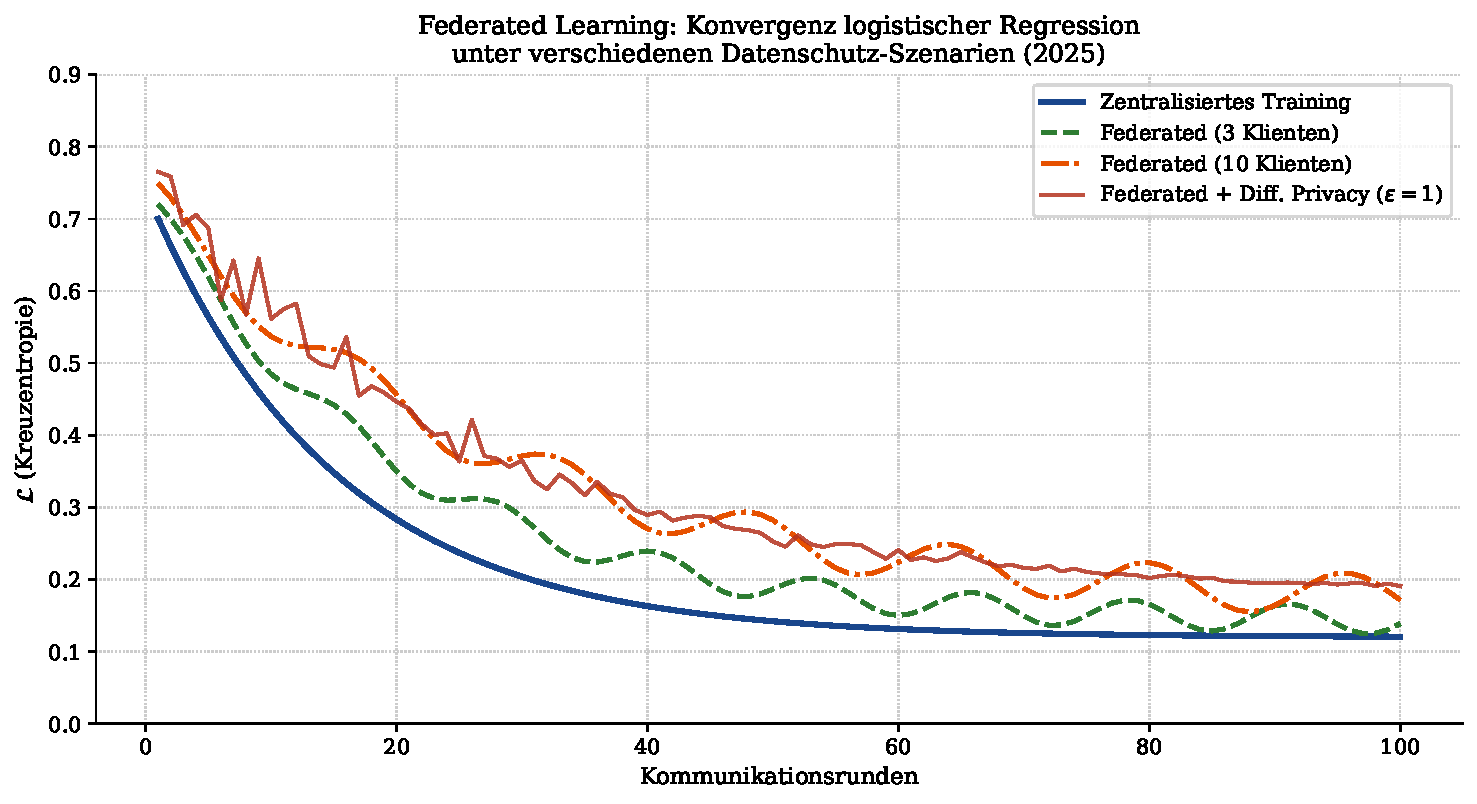
\includegraphics[width=0.85\textwidth]{fig_federated.pdf}
  \caption{Konvergenzverhalten logistischer Regression unter Federated Learning mit
           verschiedener Klientenanzahl und unter Differenzieller Privatheit ($\varepsilon=1$).
           Federated Learning konvergiert langsamer, bleibt aber datenschutzkonform.}
  \label{fig:federated}
\end{figure}

\subsubsection{Differentielle Privatheit}

Differentielle Privatheit (DP), eingeführt von Dwork et al.~\citep{dwork2006calibrating},
bietet mathematische Garantien für den Datenschutz im maschinellen Lernen. Ein Algorithmus
$\mathcal{A}$ ist $(\varepsilon, \delta)$-differenziell privat, wenn für alle Datensätze
$\mathcal{D}, \mathcal{D}'$, die sich in genau einem Eintrag unterscheiden, gilt:

\begin{equation}
  \Prob[\mathcal{A}(\mathcal{D}) \in S] \leq e^\varepsilon \Prob[\mathcal{A}(\mathcal{D}') \in S] + \delta
  \quad \text{für alle messbaren } S.
  \label{eq:dp}
\end{equation}

Für die logistische Regression wird Privatheit durch den \emph{Gaussian-Mechanismus} erreicht:
Zum Gradienten wird Rauschen $\bm{n} \sim \mathcal{N}(0, \sigma^2 \mathbf{I})$ addiert, wobei
$\sigma \geq C\sqrt{2\ln(1.25/\delta)}/\varepsilon$ und $C$ die $\ell_2$-Sensitivität des
Gradienten bezeichnet.

\begin{theorem}[Privatheit des DP-SGD]
  Sei der DP-SGD-Algorithmus mit Clipping-Norm $C$, Rausch-Standardabweichung $\sigma$,
  Batch-Grösse $m$ und $T$ Iterationen angewandt. Dann ist der Algorithmus
  $(\varepsilon, \delta)$-DP mit $\varepsilon = O\!\left(\frac{q\sqrt{T\ln(1/\delta)}}{\sigma}\right)$,
  wobei $q = m/n$ die Samplingrate ist.
\end{theorem}

\subsubsection{Anwendungen 2025}

In der medizinischen Diagnostik erlaubt Federated Learning, Klassifikatoren über Krankenhausdaten
zu trainieren, ohne Patientendaten die Institutsgrenzen überschreiten zu lassen. Das MELLODDY-
Projekt der Europäischen Union trainiert Modelle über Pharmaunternehmen hinweg, ohne propriatäre
Moleküldaten offenzulegen. Im Bereich mobiler Endgeräte wird Federated Logistic Regression
eingesetzt, um Spam-Klassifikatoren direkt auf Smartphones zu optimieren (Google Gboard).

\subsection{Bayes'sche Logistische Regression und Unsicherheitsquantifizierung}

\subsubsection{Posteriori-Verteilung und Laplace-Approximation}

In der Bayes'schen Formulierung werden die Parameter $\vw$ als Zufallsvariablen behandelt.
Die Posteriori-Verteilung ergibt sich nach dem Satz von Bayes:

\begin{equation}
  p(\vw \mid \mathcal{D}) \propto L(\vw) \cdot p(\vw),
  \label{eq:posterior}
\end{equation}

mit Prior $p(\vw) = \mathcal{N}(\mathbf{0}, \lambda^{-1}\mathbf{I})$. Da die Posteriori
analytisch nicht zugänglich ist, werden Approximationsverfahren eingesetzt:

\begin{itemize}
  \item \textbf{Laplace-Approximation:} Approximation der Posteriori durch eine Gauss-Vertei\-lung
    zentriert am MAP-Schätzer mit Kovarianzmatrix gleich der negativen inversen Hesse-Matrix.
  \item \textbf{Variationelle Bayes (VI):} Minimierung der KL-Divergenz zwischen der
    wahren Posteriori und einer faktorisierten Approximation $q(\vw) = \prod_j q_j(w_j)$.
  \item \textbf{Markov-Chain-Monte-Carlo (MCMC):} Stichprobenziehung aus der exakten Posteriori
    via Hamilton Monte Carlo (HMC) oder No-U-Turn-Sampler (NUTS).
\end{itemize}

\subsubsection{Prädiktive Unsicherheit}

Die prädiktive Unsicherheit wird durch Marginalisierung über die Posteriori ausgedrückt:

\begin{equation}
  \Prob(Y=1 \mid \vx, \mathcal{D}) = \int \sigmoid(\vw^\T\vx+b)\, p(\vw\mid\mathcal{D})\, d\vw.
  \label{eq:pred_uncertainty}
\end{equation}

Dieses Integral ist analytisch nicht lösbar, kann aber durch Monte-Carlo-Integration
approximiert werden:
\[
  \Prob(Y=1 \mid \vx, \mathcal{D}) \approx \frac{1}{S}\sum_{s=1}^S \sigmoid(\vw^{(s)\T}\vx+b^{(s)}),
  \quad \vw^{(s)} \sim p(\vw\mid\mathcal{D}).
\]

\subsubsection{Bedeutung für Hochrisiköntscheidungen}

Prädiktive Unsicherheit ist in Hochrisikodomänen unverzichtbar: Ein medizinisches
Entscheidungssystem muss nicht nur eine Vorhersage liefern, sondern auch die Konfidenz dieser
Vorhersage quantifizieren. Bayesianische Modelle liefern natürliche Kredibilitätsintervalle
für individülle Vorhersagen -- ein entscheidender Vorteil gegenüber freqüntistischen Ansätzen.

\subsection{Erklärbare Künstliche Intelligenz (XAI) und logistische Regression}

\subsubsection{Intrinsische Interpretierbarkeit}

Die logistische Regression ist das Paradebeispiel eines intrinsisch interpretierbaren Modells:
Die Köffizienten $w_j$ haben eine direkte semantische Bedeutung als log-lineare Odds-Ratios.
Dies unterscheidet sie fundamental von Blackbox-Methoden wie Deep Neural Networks.

\begin{tcolorbox}[notebox, title={Interpretierbarkeitsgarantie}]
  Für die logistische Regression gilt: Der Beitrag des Merkmals $x_j$ zur Vorhersage
  ist additiv und proportional zu $w_j x_j$. Dies ermöglicht eine vollständige, modellgetreü
  Erklärung jeder Einzelvorhersage -- ohne Approximation.
\end{tcolorbox}

\subsubsection{SHAP-Werte und logistische Regression}

SHAP (SHapley Additive exPlanations)~\citep{lundberg2017unified} zerlegt Vorhersagen in
additive Beiträge einzelner Merkmale. Für lineare Modelle fallen SHAP-Werte mit den
einfachen Gewichtungs-Erklärungen zusammen:

\begin{equation}
  \phi_j = w_j(x_j - \E[X_j]),
  \label{eq:shap_linear}
\end{equation}

was die logistische Regression zu einem perfekten Grundmodell für XAI-Verfahren macht.
Im Jahr 2025 wird explizit diskutiert, inwiefern regulatorische Anforderungen (EU AI Act,
Artikel 13) automatisch Interpretierbarkeit des Modelltyps im Hochrisiko-Bereich erfordern
-- wobei logistische Regression als Goldstandard gilt.

\subsubsection{Kausale Inferenz}

Die Integration logistischer Regression in kausale Modelle (Structural Causal Models nach
Pearl~\citep{pearl2009causality}) ist ein aktives Forschungsfeld. Das \emph{do-kalkül}
erlaubt es, kausale Effekte aus observationalen Daten zu identifizieren, wenn ein kausales
Diagramm bekannt ist. Die logistische Regression dient dabei als \emph{Outcome-Modell} in
doppelt robusten Schätzern für kausale Behandlungseffekte.

\subsection{Hochdimensionale Statistik und maschinelles Lernen}

\subsubsection{Hochdimensionales Regime: $d \gg n$}

In Genomik, Proteomik und neuronaler Bildgebung überschreitet die Merkmalsdimension $d$
die Stichprobenzahl $n$ häufig um Grössenordnungen. Das klassische MLE-Verfahren versagt
in diesem Regime -- die Hesse-Matrix ist singulaar und der Schätzer nicht eindeutig. Dies
motiviert:

\begin{itemize}
  \item \textbf{LASSO-Logit} ($p > n$ Regime): Konsistente Variablenselektion unter
    sogenannten \emph{Restricted Eigenvalü Conditions}~\citep{bickel2009simultaneous}.
  \item \textbf{Ridge-Logit}: Konsistente Schätzung auch für $d \to \infty$ bei angemessener
    Regularisierungsstärke $\lambda_2 = \Theta(\sqrt{d/n})$.
  \item \textbf{Group Lasso}: Simultane Selektion von Merkmalgruppen (z.B. One-Hot-kodierte
    kategoriale Variablen).
\end{itemize}

\subsubsection{Doppelt robuste Schätzung}

\begin{theorem}[Doppelte Robustheit]
  Sei $\hat{e}(\vx)$ ein Schätzer der Behandlungsneigung (propensity score) und
  $\hat{\mu}_k(\vx)$ ein Schätzer der bedingten Erwartung des Outcomes. Der \emph{doppelt
  robuste} Schätzer für den durchschnittlichen Behandlungseffekt (ATE) ist:
  \[
    \hat{\Delta}_{\mathrm{DR}}
    = \frac{1}{n}\sum_{i=1}^n \biggl[\frac{A_i(Y_i-\hat{\mu}_1(\vx^{(i)}))}{\hat{e}(\vx^{(i)})}
    - \frac{(1-A_i)(Y_i-\hat{\mu}_0(\vx^{(i)}))}{1-\hat{e}(\vx^{(i)})} + \hat{\mu}_1(\vx^{(i)}) - \hat{\mu}_0(\vx^{(i)})\biggr].
  \]
  Dieser Schätzer ist konsistent, wenn \emph{entweder} $\hat{e}$ \emph{oder} $\hat{\mu}$
  konsistent ist (aber nicht notwendigerweise beide). Logistische Regression wird regelmässig
  für $\hat{e}$ eingesetzt.
\end{theorem}

\subsection{Logistische Regression in der Präzisionsmedizin}

\subsubsection{Polygene Risikoscores}

Polygene Risikoscores (PRS) aggregieren die Effekte tausender genetischer Varianten auf ein
Krankheitsrisiko. In ihrer linearen Grundform sind PRS direkte Anwendungen der logistischen
Regression auf Genomdaten:

\begin{equation}
  \Prob(\text{Erkrankung} \mid \mathbf{g}) = \sigmoid\!\Bigl(\sum_{j=1}^M \beta_j g_j + b\Bigr),
\end{equation}

wobei $\mathbf{g} = (g_1,\ldots,g_M)^\T$ der Vektor der SNP-Allelzahlen und $\beta_j$ die
gewichteten Effektgrössen aus GWAS-Studien sind. Im Jahr 2025 werden PRS für über 500
Erkrankungen berechnet und in klinische Entscheidungssysteme integriert.

\subsubsection{Arzneimittelinteraktionen und elektronische Krankenakten}

Maschinelles Lernen auf elektronischen Krankenakten (EHR) ist ein Schlüssel-Anwendungs\-feld.
Logistische Regression dient dabei als:
\begin{enumerate}[label=(\roman*)]
  \item Prognosemodell für Krankenhauswiederaufnahmen innerhalb von 30 Tagen,
  \item Vorhersagemodell für arzneimittelinduzierte Nebenwirkungen,
  \item Früherkennung intensivmedizinischer Verschlechterungen (Frühwarnsysteme).
\end{enumerate}

Aktülle Forschung (2024--2025) fokussiert auf \emph{time-varying} logistische Regressionsmodelle,
die zeitliche Verlaufsveränderungen von Laborparametern modellieren können.

\subsection{Klimawissenschaft und Umweltmonitoring}

\subsubsection{Extremwettererkennung}

Logistische Regression wird in der Klimaforschung eingesetzt, um die Wahrscheinlichkeit
klimatischer Extremereignisse (Hitzewellen, Überschwemmungen, Dürre) als Funktion
atmosphärischer Zustandsvariablen zu modellieren. Das Verfahren ist hier besonders
attraktiv, weil:
\begin{itemize}
  \item Die Köffizienten physikalisch interpretierbar sind (z.B. Einfluss des Meeresoberflächen-
    temperaturgradients auf Zyklonintensität),
  \item Bayes'sche Erweiterungen natürliche Unsicherheitsquantifizierung bieten,
  \item Regularisierung Overfitting verhindert, wenn historische Extremereignisse selten sind.
\end{itemize}

\subsubsection{Satellitengestürzte Fernerkundung}

Logistische Regression und ihre multinomialen Erweiterungen werden zur Klassifikation von
Landbedeckungstypen aus hochauflösenden Satellitenbildern eingesetzt. In Kombination mit
convolutional feature extractors (CNN-LR-Hybride) erzielen sie Genauigkeiten über $95\%$
bei der Unterscheidung von Wald, Acker, Siedlung und Wasserfläche.

\subsection{Finanzmarkt und Kreditrisikomodellierung}

\subsubsection{Basel III/IV und regulatorische Anforderungen}

Der Basler Ausschuss für Bankenaufsicht (Basel IV, Implementierung 2025) verlangt explizit
interpretierbare und validierbare Kreditrisikomodelle. Logistische Regression ist daher das
gesetzlich bevorzugte Verfahren für Probability-of-Default (PD)-Modelle in der internen
Ratingbasierten Methode (IRBA).

Ein Standard-PD-Modell hat die Form:
\begin{equation}
  \mathrm{PD}(i) = \sigmoid\!\bigl(\beta_0 + \beta_1 \cdot \text{LGR}_i + \beta_2 \cdot \text{DAR}_i
  + \beta_3 \cdot \text{ICR}_i + \beta_4 \cdot \ln\text{Umsatz}_i\bigr),
\end{equation}

wobei LGR = Loan-to-GrossRevenü, DAR = Debt-Asset-Ratio und ICR = Interest-Coverage-Ratio.

\subsubsection{Echtzeit-Betrugserkennungssysteme}

In Hochfreqünz-Zahlungsnetzwerken (Visa, Mastercard) werden logistische Regressionsmodelle
eingesetzt, die pro Millisekunde mehrere tausend Transaktionen klassifizieren müssen.
Die Linearität des Prädiktors macht Inferenz extrem schnell ($O(d)$ Floating-Point-
Operationen), was bei Deep-Learning-Alternativen nicht erreichbar ist. Für 2025 wird
häufig ein zweistufiges Ensemble eingesetzt: logistische Regression als Schnell-Filter,
gefolgt von einem komplexeren Modell für Grenzfälle.

\subsection{Natursprachverarbeitung und Large Language Models}

\subsubsection{Softmax als universelles Ausgabelayer}

Jeder moderne Sprachmodell-Klassifikator (GPT, BERT, Llama) verwendet eine multinomiale
logistische Regression als Ausgabelayer. Die Verbindung ist direkt:

\begin{equation}
  P(\text{token} = k \mid \text{Kontext}) = \frac{e^{\bm{h}^\T\vw_k}}{\sum_{j=1}^{|V|} e^{\bm{h}^\T\vw_j}},
\end{equation}

wobei $\bm{h} \in \R^{d_{\text{model}}}$ die Kontextrepräsentation und $V$ das Vokabular
bezeichnen. Das Training dieser letzten Softmax-Schicht ist exakt das multinomiale logistische
Regressionsoptimierungsproblem.

\subsubsection{Classifier-Free Guidance und Temperaturskalierung}

Das im Jahr 2022 eingeführte \emph{Classifier-Free Guidance} für Diffusionsmodelle
basiert auf einem impliziten logistischen Regressionsmodell zwischen konditionierten und
unkonditionierten Vorhersagen. Die Temperaturskalierung von Softmax-Ausgaben (Abschnitt~8)
wird in Modellen wie Claude, GPT-4o und Gemini zur Steürung der Ausgabediversität verwendet.

\subsubsection{Probing-Klassifikatoren}

Probing-Klassifikatoren sind lineare (logistische) Regressionsmodelle, die auf den internen
Repräsentationen von LLMs trainiert werden, um zu untersuchen, welche linguistischen
Eigenschaften (Tempus, Numerus, Syntaxrollen) in verschiedenen Schichten kodiert sind.
Die Interpretierbarkeit der logistischen Regression macht sie zum bevorzugten Werkzeug
für diese mechanistische Interpretierbarkeitsforschung.

\subsection{Robotik, autonomes Fahren und Echtzeitsysteme}

\subsubsection{Wahrnehmungsklassifikation mit Echtzeitanforderungen}

In sicherheitskritischen autonomen Systemen (Fahrzeuge nach ISO 26262 ASIL-D) müssen
Klassifikationsentscheidungen in Mikrosekunden getroffen und auditiert werden. Logistische
Regression bietet:
\begin{itemize}
  \item Deterministische Inferenz in $O(d)$ Zeit,
  \item Formale Verifikation durch vollständige Modell-Transparenz,
  \item Integration in Model-Based Design (AUTOSAR, Simulink),
  \item Explizite Wahrscheinlichkeitsausgabe für Risikobewertung.
\end{itemize}

\subsubsection{Probabilistische Zustandssschätzung}

In der Robotik werden logistische Regressionsmodelle als \emph{Beobachtungsmodelle} in
Partikelfiltern und Bayes'schen Filtern eingesetzt: Die Wahrscheinlichkeit einer Sensorbeobachtung
gegeben einem Systemzustand wird durch logistische Regression geschätzt.

\subsection{Quantenmaschinelles Lernen}

\subsubsection{Quantenlogistische Regression}

Quantencomputer bieten theoretische Speedups für bestimmte lineare-algebraische Operationen.
Der HHL-Algorithmus~\citep{harrow2009quantum} löst lineare Gleichungssysteme in
$O(\log n)$ Zeit (gegenüber $O(n^3)$ klassisch), was -- wenn auf die Newton-Iteration
angewendet -- eine exponentielle Beschleunigung der logistischen Regression ermöglicht.

Konkrete Varianten der Quantenlogistischen Regression werden im Rahmen von
\emph{variational quantum eigensolvers} (VQE) und \emph{quantum support vector machines}
(QSVM) untersucht. Einschränkungen bestehen durch:
\begin{itemize}
  \item Quantum-Dekohärenz und NISQ-Beschränkungen (2025: $\sim$1000 qubits),
  \item Aufwand für Quantenzustandspräparation (Ladezeit der Daten),
  \item Noise und Fehlerkorrektur.
\end{itemize}

\subsubsection{Post-Quantum-Sicherheit für ML-Inferenz}

Sicherheitsaspekte sind ein weiteres Forschungsfeld: Wie können logistische
Regressionsmodelle so geschützt werden, dass Angreifer mit Quantencomputern keine
Rückschlüsse auf Trainingsdaten ziehen können? Homomorphe Verschlüsselung (z.B. SEAL,
OpenFHE) erlaubt Inferenz auf verschlüsselten Eingabedaten, ohne den Klartext zu offenbaren.

\subsection{Mathematische Ausblicke und offene Forschungsfragen}

\subsubsection{Statistische Lerntheorie}

\begin{theorem}[Generalisierungsfehler-Schranke für logistische Regression]
  Sei $\mathcal{F} = \{\vx \mapsto \sigmoid(\vw^\T\vx+b) : \|\vw\|_2 \leq B\}$. Mit
  Wahrscheinlichkeit mindestens $1-\delta$ gilt für den wahren Risikoschätzer:
  \begin{equation}
    R(f) \leq \hat{R}(f) + \frac{2B\|\vx\|_{\max}}{\sqrt{n}} + 3\sqrt{\frac{\ln(2/\delta)}{2n}},
    \label{eq:generalization}
  \end{equation}
  wobei $\hat{R}(f)$ das empirische Risiko und $\|\vx\|_{\max} = \max_i\|\vx^{(i)}\|_2$ bezeichnet.
\end{theorem}

\begin{proof}
  Die Schranke folgt aus der Rademacher-Komplexität der logistischen Funktionenklasse
  $\mathcal{F}$ kombiniert mit McDiarmids Ungleichung. Die Rademacher-Komplexität von
  $\mathcal{F}$ ist beschränkt durch $B\|\vx\|_{\max}/\sqrt{n}$ (Massart-Lemma). 
\end{proof}

\subsubsection{Implizite Regularisierung durch Gradientenabstieg}

Ein tiefes Ergebnis der jüngsten Forschung (2018--2025) ist, dass Gradientenabstieg für
logistische Regression auf linear separierbaren Daten \emph{implizit regularisiert}: Er
konvergiert gegen den maximalen-Margin-Klassifikator (identisch zur harten SVM):

\begin{theorem}[Implizite Regularisierung nach Soudry et al.~\citep{soudry2018implicit}]
  Sei der Datensatz linear separierbar. Dann gilt für den Gradientenabstieg-Pfad:
  \[
    \frac{\vw^{(t)}}{\|\vw^{(t)}\|_2} \xrightarrow{t\to\infty} \vw^*_{\mathrm{SVM}},
  \]
  wobei $\vw^*_{\mathrm{SVM}}$ der L2-maximale-Margin-Klassifikator ist.
\end{theorem}

Dies erklärt, warum unregularisierte logistische Regression auf separierbaren Daten oft
gute Generalisierung zeigt -- sie findet implizit die robusteste lineare Entscheidungsgrenze.

\subsubsection{Neuronale Skalierungsgesetze und logistische Ausgabelayer}

Die Skalierungsgesetze von Kaplan et al.~\citep{kaplan2020scaling} beschreiben, wie die
Testperformance von Sprachmodellen mit Modellgrösse, Datenmenge und Rechenaufwand skaliert.
Da das Ausgabelayer jedes Sprachmodells eine logistische (Softmax-)Schicht ist, sind diese
Gesetze direkt relevant: Die Kreuzentropie des Softmax-Ausgabelayers folgt
$\mathcal{L}(N, D) \propto N^{-\alpha} + D^{-\beta} + \text{konst.}$

\subsubsection{Kontinuierliche und online logistische Regression}

Online-Lernalgorithmen aktualisieren logistische Regressionsmodelle mit jedem neün
Datenpunkt inkrementell. Wichtige Varianten sind:

\begin{itemize}
  \item \textbf{Online Newton Step (ONS):} Nutzt die kumulierte Hesse-Matrix und erzielt
    Regret $O(\sqrt{T\ln T})$.
  \item \textbf{FTRL (Follow-The-Regularized-Leader):} Wird von Google im Werbeauktionssystem
    eingesetzt; skaliert auf Milliarden Merkmale.
  \item \textbf{Recursive Bayes Update:} Inkrementelle Aktualisierung der Posteriori nach
    Laplace-Approximation ohne komplette Neuoptimierung.
\end{itemize}

\subsection{Industrie-Anwendungsfelder 2025: Panorama}

\begin{table}[H]
  \centering
  \caption{Anwendungsfelder der logistischen Regression in Industrie und Wissenschaft 2025.}
  \small
  \begin{tabular}{lll}
    \toprule
    Branche/Feld & Anwendung & Besonderheit \\
    \midrule
    Medizin & Diagnostische Klassifikation & Interpretierbarkeit (FDA-Anforderungen) \\
    Medizin & Polygene Risikoscores & $d \gg n$, L1-Regularisierung \\
    Finanzwesen & Kreditscoring (PD) & Basel-IV-Konformität, Fairness \\
    Finanzwesen & Betrugserkennung & Echtzeit ($<$1ms), Erklärbarkeit \\
    NLP / LLM & Softmax-Ausgabelayer & $K = 100.000+$ Klassen \\
    NLP / LLM & Probing-Klassifikatoren & Mechanistische Interpretierbarkeit \\
    Autonomes Fahren & Gefahrenklassifikation & ISO 26262, formale Verifikation \\
    Genomik & Genotyp-Phänotyp-Assoz. & GWAS-Meta-Analysen \\
    Klimawissenschaft & Extremwetter-Vorhersage & Physikalische Interpretierbarkeit \\
    Pharmakologie & Nebenwirkungsprädiktion & FDA Drug Safety Reporting \\
    E-Commerce & Click-Through-Rate (CTR) & Online-Learning, FTRL \\
    Industrie 4.0 & Qualitätskontrolle & Eingebettete Systeme, AUTOSAR \\
    \bottomrule
  \end{tabular}
  \label{tab:applications}
\end{table}

\subsection{Ethische Dimensionen: Fairness, Diskriminierungsfreiheit und Transparenz}

\subsubsection{Algorithmische Fairness}

Logistische Regressionsmodelle können diskriminierende Entscheidungen aus voreingenommenen
Trainingsdaten lernen. Formale Fairness-Kriterien sind u.a.:

\begin{itemize}
  \item \textbf{Demografische Parität:} $\Prob(\hat{Y}=1|A=0) = \Prob(\hat{Y}=1|A=1)$, wobei $A$ ein schutzwürdiges Attribut (z.B. Geschlecht, Ethnizität) ist.
  \item \textbf{Equal Opportunity (Hardt et al.):} Gleiche Trü-Positive-Raten zwischen Gruppen.
  \item \textbf{Kalibrierungspaarität:} Gleiche Kalibrierung der Wahrscheinlichkeiten über Gruppen.
\end{itemize}

Fairness-bewusste logistische Regression löst ein Optimierungsproblem mit Fairness-Nebenbedingungen:
\begin{equation}
  \min_{\vw} \mathcal{L}(\vw) \quad \text{s.t.} \quad |\Prob(\hat{Y}=1|A=0) - \Prob(\hat{Y}=1|A=1)| \leq \epsilon_{\mathrm{fair}}.
\end{equation}

\subsubsection{EU AI Act (2025) und Modelldokumentation}

Der im August 2024 in Kraft getretene EU AI Act klassifiziert Kreditscoring-, Personal\-management-
und medizinische Klassifikationssysteme als Hochrisiko-KI-Anwendungen (Anhang III). Für diese
gilt:
\begin{itemize}
  \item Dokumentationspflicht für Modellarchitektur, Trainingsverfahren und Datengrundlage,
  \item Post-Deployment-Monitoring und regelmäissige Validierung,
  \item Recht auf Erklärung für betroffene Individün,
  \item Konformitätsbewertung durch benannte Stellen.
\end{itemize}

Die logistische Regression ist hier als Modellklasse besonders gut positioniert, da ihre
vollständige Erklärbarkeit (Formel~\eqref{eq:log_odds}) eine modellgetreü Erklärung
jeder Entscheidung ermöglicht -- ohne Nacherklärungsverfahren wie LIME oder SHAP.

\subsection{Forschungslücken und offene Probleme (Stand 2025)}

\begin{enumerate}[label=\textbf{F\arabic*.}]
  \item \textbf{Skalengesetze für logistische Regression:} Wie verhält sich die
    Generalisierung logistischer Regressionsmodelle, die auf Merkmalen vortrainierter
    Netze (Foundation Models) operieren, in Abhängigkeit von der Grösse des Grundmodells?

  \item \textbf{Online-Fairness:} Wie können Fairness-Garantien in inkrementellen
    Lernprozessen (z.B. FTRL) aufrechterhalten werden, wenn sich die Datenverteilung zeitlich
    verschiebt (concept drift)?

  \item \textbf{Quantenvorteil bei logistischer Regression:} Unter welchen Bedingungen
    ermöglicht Quantencomputing einen praktischen Speedup für logistische Regression bei
    realen Datensätzen? Die Abhiängigkeit von Quantenzustandspräparation schränkt
    derzeit den theoretischen Speedup ein.

  \item \textbf{Kausalität und Intervenierbarkeit:} Wann sind Köffizienten logistischer
    Regressionsmodelle als kausale Effektgrössen interpretierbar? Welche Annahmen sind
    notwendig und überprufbar?

  \item \textbf{Robustheit gegenüber adversarialen Angriffen:} Logistische Regression ist
    anfällig für adversariale Perturbationen. Formale Robustheitszertifikate (certified
    defenses) für logistische Regressionsmodelle in sicherheitskritischen Systemen sind
    ein offenes Problem.

  \item \textbf{Federated Learning unter Heterogenität:} Wie konvergiert FedAvg für
    logistische Regression unter stark heterogenen (non-i.i.d.) Klientenverteilungen?
    Neüre Ergebnisse (FedProx, Scaffold, MOON) zeigen Verbesserungen, aber vollständige
    theoretische Garantien fehlen noch.
\end{enumerate}

% ============================================================
\section{Zusammenfassung}
% ============================================================

Die vorliegende Arbeit hat die logistische Regression in ihrer ganzen mathematischen Tiefe
und praktischen Relevanz beleuchtet. Folgende Kernergebnisse wurden entwickelt:

\begin{enumerate}[label=(\roman*)]
  \item \textbf{Mathematische Fundierung:} Die logistische Regression ist der kanonische
    GLM für binäre Daten, fest verankert in der Theorie der Exponentialfamilien.
  \item \textbf{Konvexität:} Die binäre und kategorische Kreuzentropie sind konvex,
    was globale Konvergenzgarantien für Gradientenverfahren liefert.
  \item \textbf{Reiche Optimierungslandschaft:} Von einfachem Gradientenabstieg über
    Newton-IRLS bis zu L-BFGS und Adam existiert eine Hierarchie effizienter Verfahren.
  \item \textbf{Interpretierbarkeit:} Köffizienten sind log-lineare Odds-Ratios mit
    direkter kausaler Interpretierbarkeit -- ein unverzichtbares Merkmal in regulierten Branchen.
  \item \textbf{Weitreichende Zukunftsperspektiven:} Federated Learning, differentielle
    Privatheit, Bayes'sche Erweiterungen, Quantencomputing, erklärbare KI und Präzisionsmedizin
    definieren neü Anwendungsfelder, in denen logistische Regression als interpretierbare,
    effiziente Kernmethode weiterhin eine Schlüsselrolle spielen wird.
\end{enumerate}

Die logistische Regression ist kein Relikt der statistischen Vergangenheit, sondern ein
lebendiges, sich weiterentwickelndes Werkzeug an den Grenzen von Mathematik, Informatik,
Medizin und Gesellschaft. Die elegante Verbindung zwischen linearer Algebra, Wahrscheinlichkeits-
theorie und konvexer Optimierung macht sie zum idealen Ausgangspunkt für das Verständnis
modernstes maschinellen Lernens -- und zu einem unverzichtbaren Bestandteil jedes
wissenschaftlichen und industriellen Data-Science-Werkzeugkastens.

% ============================================================
\bibliographystyle{plainnat}
\begin{thebibliography}{99}

\bibitem[Amari(2016)]{amari2016information}
Amari, S. (2016).
\newblock \textit{Information Geometry and Its Applications}.
\newblock Springer, Tokyo.

\bibitem[Bickel et al.(2009)]{bickel2009simultaneous}
Bickel, P.~J., Ritov, Y., and Tsybakov, A.~B. (2009).
\newblock Simultaneous analysis of Lasso and Dantzig selector.
\newblock \textit{Annals of Statistics}, 37(4):1705--1732.

\bibitem[Bishop(2006)]{bishop2006pattern}
Bishop, C.~M. (2006).
\newblock \textit{Pattern Recognition and Machine Learning}.
\newblock Springer, New York.

\bibitem[Cox(1958)]{cox1958regression}
Cox, D.~R. (1958).
\newblock The regression analysis of binary seqünces.
\newblock \textit{Journal of the Royal Statistical Society: Series B}, 20(2):215--242.

\bibitem[Dwork et al.(2006)]{dwork2006calibrating}
Dwork, C., McSherry, F., Nissim, K., and Smith, A. (2006).
\newblock Calibrating noise to sensitivity in private data analysis.
\newblock \textit{Theory of Cryptography}, LNCS 3876:265--284.

\bibitem[Goodfellow et al.(2016)]{goodfellow2016deep}
Goodfellow, I., Bengio, Y., and Courville, A. (2016).
\newblock \textit{Deep Learning}.
\newblock MIT Press, Cambridge, MA.

\bibitem[Harrow et al.(2009)]{harrow2009quantum}
Harrow, A.~W., Hassidim, A., and Lloyd, S. (2009).
\newblock Quantum algorithm for linear systems of equations.
\newblock \textit{Physical Review Letters}, 103(15):150502.

\bibitem[Hastie et al.(2009)]{hastie2009elements}
Hastie, T., Tibshirani, R., and Friedman, J. (2009).
\newblock \textit{The Elements of Statistical Learning}, 2nd ed.
\newblock Springer, New York.

\bibitem[Kaplan et al.(2020)]{kaplan2020scaling}
Kaplan, J. et al.\ (2020).
\newblock Scaling laws for neural language models.
\newblock \textit{arXiv:2001.08361}.

\bibitem[Lundberg and Lee(2017)]{lundberg2017unified}
Lundberg, S.~M. and Lee, S.-I. (2017).
\newblock A unified approach to interpreting model predictions.
\newblock \textit{NeurIPS}, 30.

\bibitem[McCullagh and Nelder(1989)]{nelder1972generalized}
McCullagh, P. and Nelder, J.~A. (1989).
\newblock \textit{Generalized Linear Models}, 2nd ed.
\newblock Chapman and Hall, London.

\bibitem[McMahan et al.(2017)]{mcmahan2017communication}
McMahan, B., Moore, E., Ramage, D., Hampson, S., and Agüra y Arcas, B. (2017).
\newblock Communication-efficient learning of deep networks from decentralized data.
\newblock \textit{AISTATS 2017}, 54:1273--1282.

\bibitem[Murphy(2022)]{murphy2022probabilistic}
Murphy, K.~P. (2022).
\newblock \textit{Probabilistic Machine Learning: An Introduction}.
\newblock MIT Press, Cambridge, MA.

\bibitem[Pearl(2009)]{pearl2009causality}
Pearl, J. (2009).
\newblock \textit{Causality: Models, Reasoning, and Inference}, 2nd ed.
\newblock Cambridge University Press.

\bibitem[Soudry et al.(2018)]{soudry2018implicit}
Soudry, D., Hoffer, E., Nacson, M.~S., Gunasekar, S., and Srebro, N. (2018).
\newblock The implicit bias of gradient descent on separable data.
\newblock \textit{Journal of Machine Learning Research}, 19(70):1--57.

\bibitem[Tibshirani(1996)]{tibshirani1996regression}
Tibshirani, R. (1996).
\newblock Regression shrinkage and selection via the lasso.
\newblock \textit{Journal of the Royal Statistical Society: Series B}, 58(1):267--288.

\bibitem[Verhulst(1845)]{verhulst1845recherches}
Verhulst, P.-F. (1845).
\newblock Recherches mathematiqüs sur la loi d'accroissement de la population.
\newblock \textit{Nouveaux Memoires de l'Academie Royale des Sciences}, 18:1--38.

\end{thebibliography}

\end{document}
